\documentclass[a4paper,polish,12pt,twoside]{article}
\usepackage[utf8]{inputenc}	
\usepackage[T1]{fontenc}
\usepackage[inner=3.5cm,outer=2.5cm,top=2.5cm,bottom=2.5cm]{geometry}
\usepackage[polish]{babel}
\usepackage[polish]{babelbib}
\usepackage{polski}	
\usepackage{amsmath}	
\usepackage{amsfonts}
\usepackage{color}
\usepackage{titlesec}
\usepackage{microtype}
\usepackage{cite}
\usepackage{float}
\usepackage{graphicx}
\usepackage{indentfirst}
\usepackage{listings}
\usepackage[nottoc]{tocbibind}
\usepackage{bookman}
\usepackage[font=small,labelfont=bf]{caption}

% Proper interline
\newcommand{\WorkLineSpread}{1.5}
\linespread{\WorkLineSpread}

% Listing parameters
\renewcommand{\lstlistingname}{Listing}
\definecolor{javared}{rgb}{0.6,0,0} % strings
\definecolor{javagreen}{rgb}{0.25,0.5,0.35} % comments
\definecolor{javapurple}{rgb}{0.5,0,0.35} % keywords
\definecolor{javadocblue}{rgb}{0.25,0.35,0.75} % javadoc
\floatstyle{plaintop} \newfloat{listing}{top}{lop}
\lstset{language=Java,
basicstyle=\ttfamily,
keywordstyle=\color{javapurple}\bfseries,
stringstyle=\color{javared},
commentstyle=\color{javagreen},
morecomment=[s][\color{javadocblue}]{/**}{*/},
numbers=none, stepnumber=2, tabsize=4, showspaces=false, showstringspaces=false}

% Comma at the end of paragraph number
\let \savenumberline \numberline \def \numberline#1{\savenumberline{#1.}}
\titlelabel{\thetitle.\quad}

% Clearing page after each section
\def \docsection#1{\clearpage\section{#1}}

% Table caption on top, fixing Babel calling tables "tablice" not "tabele"
\floatstyle{plaintop} \restylefloat{table}
\captionsetup{belowskip=4pt, aboveskip=4pt}
\addto\captionspolish{\renewcommand{\tablename}{Tabela}%
						         \renewcommand{\listtablename}{Spis tabel}}

\begin{document}
	\begin{titlepage}
	
	\vspace{2cm}

	\centering \hspace*{1.5cm}
\includegraphics[width=14cm]{mojpieknywydzial}

	\vspace{2.5cm}

	\centering {\Large Katedra Informatyki i Automatyki}

	\vspace{2cm} 

	\centering {\large \textbf{Piotr Maślanka}} \\
	\centering {\large Rozproszona baza danych \\ systemu kontrolno-pomiarowego}

	\vspace{5cm}

	\centering \large \textbf{Praca dyplomowa inżynierska}

	\vspace{2.5cm}

	\linespread{1}
	Opiekun pracy: \\
	dr inż. Andrzej Stec
	\linespread{\WorkLineSpread}
	\vspace{1cm}

	\large \textbf{Rzeszów 2015}

	\end{titlepage}

	\newpage
    
	\tableofcontents

	\newpage

    \docsection{Wstęp}
	Jedną z podstawowych cech charakteryzujących systemy kontrolno-pomiarowe jest to, że dotyczą one monitorowania procesów zmiennych w czasie. Kontrolowanymi wielkościami mogą być: natężenie prądu, wartość napięcia, temperatura, ciśnienie, zużycie paliwa i wiele innych. Zmiany ich wartości mogą być wywołane zamierzonymi działaniami operatora, ale także różnego rodzaju zakłóceniami lub awariami. Do analizy poprawności funkcjonowania takich systemów konieczne jest często rejestrowanie danych bieżących w dłuższym okresie czasu i przechowywanie ich w bazach danych. Jednocześnie, wraz ze wzrostem liczby oraz złożoności nowo projektowanych systemów, ilość danych niezbędnych do przechowywania stale wzrasta. Istnieje więc potrzeba opracowywania rozwiązań, które będą zapewniać efektywny i niezawodny dostęp do danych, minimalizując jednocześnie ryzyko ich utraty.

Bazy danych typu Big Data stanowią stosunkowo nowy trend w informatyce. Służą one do przechowywania danych strukturalnych o objętości zbyt dużej, by możliwa była ich obróbka tradycyjnymi systemami. Charakteryzują się one rozproszeniem danych na wiele węzłów w klastrze. Dzięki temu zapewniają zwiększoną prędkość odczytu i tolerancję na awarię. Znaczna część istniejących na rynku rozwiązań wewnętrznie bazuje na ideach podejścia Big Data, gdyż na chwilę obecną jedynie ono jest w stanie zapewnić również wymagane właściwości wydajnościowe. Nie tylko one są istotne, gdyż od rozwiązania takiego oczekuje się szeregu specyficznych właściwości. Baza taka musi być w stanie przetworzyć żądaną ilość danych w określonym czasie, zależnym od rozwiązania. Dodatkowymi wymaganiami jest odporność na awarie, zwłaszcza w systemie scentralizowanym, gdzie awaria krytycznego komponentu mogłaby spowodować niedostępność całej usługi.

Podstawowymi jednostkami w bazach systemów kontrolno-pomiarowych są szeregi czasowe\footnote{ciągi informacji uporządkowane w czasie}, często odpowiadające jednemu czujnikowi w systemie automatyki. Zapisują one wartości takiego sensora systemu automatyki w postaci ciągu par stempel czasowy --- wartość zmierzona. Stworzone w ten sposób szeregi zawierają dane na temat przebiegu danego procesu technologicznego w czasie. Są więc niezbędne dla analizy poprawności pracy systemu. Można je również wykorzystywać w celu bardziej złożonej analizy (np. korelacyjnej) mającej na celu osiągnięcie założonych przez operatora celów, takich jak optymalizacja pracy systemu, kosztów lub badań nad samym procesem technologicznym. Można też na ich podstawie ustalić, kiedy system ulegnie awarii. Mogą być to nawet proste metody, takie jak sprawdzanie błędu względnego między dwoma wartościami, czy bardziej skomplikowane, jak rachunek całkowy i metody korelacji krzyżowej. Częstym zjawiskiem jest stosowanie złożonych analiz, obciążających bazę pod względem ilości odczytów. Musi ona więc pozwalać zarówno na obsłużenie rejestracji dużej ilości danych, jak i na późniejszy dostęp do nich. Dlatego właśnie dobra baza danych przechowująca dane generowane przez system pomiarowy jest kluczowym składnikiem wielu systemów automatyki. 

\textbf{Celem pracy jest} opracowanie rozwiązania bazodanowego umożliwiającego gromadzenie danych pomiarowych pochodzących z wielu niedużych systemów automatyki, takich jak kotłownie czy węzły cieplne, w sposób zapewniający ciągłość i niezawodność pracy systemu. Jednocześnie, dane zgromadzone w bazie zapisywane powinny być sposób pozwalający na ich swobodny odczyt, umożliwiając operatorowi systemu przeprowadzanie analiz i sporządzanie wykresów.

Rozwiązanie bazodanowe musi być w stanie sprostać wymaganiom dużego rozproszonego systemu kontrolno-pomiarowego do nadzorowania znacznej ilości oddzielonych systemów ogrzewania takich jak kotłownie czy węzły cieplne. Przede wszystkim musi  być w stanie obsłużyć obciążenie opisane w p. \ref{sec:data_quantity_analysis}. Dodatkowo, musi ono być odporne na awarię pojedynczego węzła, nie wpływając negatywnie na poprawność i istotną jakość działania systemu. Warunkuje to jego rozproszony charakter. Wymagana jest również, ze względu na stały rozwój systemu, możliwość modyfikowania tego rozwiązania w późniejszym czasie.

Opracowywane rozwiązanie jest przygotowywane z myślą o jego praktycznym wykorzystaniu. Autor niniejszej pracy zamierza je w przyszłości zastosować do gromadzenia danych w pracującym już systemie kontrolno-pomiarowym SMOK\footnote{System Monitoringu Odległych Kotłowni}\cite{smok} służącym do nadzorowania wielu odległych instalacji techniki grzewczej w całej Polsce. Operatorem systemu jest jedna z rzeszowskich firm.

System SMOK jest rozwiązaniem, które cały czas dynamicznie się rozwija. Ze względu na chęć sprawowania kontroli nad włanością intelektualną, również baza danych stanowiąca jego istotny element, została zaplanowana jako autorskie rozwiązanie. Baza danych, która ma stanowić krytyczny komponent, musi również być w stanie sprostać temu rozwojowi. Przewiduje się, że także ona będzie w przyszłości dostosowywana do zmieniających się potrzeb systemu. Pozostałe, techniczne własności rozwiązania zostały ustalone w drodze analizy wymagań.

\textbf{W ramach pracy wykonano }następujące zadania cząstkowe:
\begin{itemize}
	\item przeprowadzono analizę wymagań systemu dotyczących obciążenia, prędkości pozyskiwania danych i ustalenia wolumenu danych, które system będzie przetwarzał,
	\item zapoznano się z istniejącymi podobnymi opracowaniami oraz metodami rozwiązywania zasadniczych problemów występujących w tym zagadnieniu,
	\item opracowano i zaprogramowano od postaw rozwiązanie, które może zapewniać żądaną funkcjonalność,
	\item przeprowadzono testy weryfikujące stosowalność bazy w systemie SMOK oraz określające charakterystykę jego skalowalności,
	\item sprzężono rozwiązanie z testową instalacją systemu SMOK.
\end{itemize}

Omawiane w pracy zagadnienia zostały podzielone na pięć części, z czego pierwsza dotyczy ogólnego sformułowania problemu, a pozostałe poświęcone są opisowi opracowanego rozwiązania.

W rozdziale 2 opisano ogólnie problem tworzenia rozproszonej bazy danych systemu kontrolno-pomiarowego, wymagania stawiane takim rozwiązaniom oraz istniejące rozwiązania. Opisano również zagadnienia rozproszenia, skalowalności i wyboru technologii za pomocą której można zbudować taką bazę.

W rozdziale 3 scharakteryzowano system kontrolno-pomiarowy, dla którego budowane jest zaproponowane rozwiązanie, przedstawiono wymagania oraz planowane do uzyskania efekty. Dodatkowo zawiera on opis architektury rozwiązania oraz sposób poradzenia sobie z kluczowymi problemami.

Rozdział 4 zawiera szczegółowy opis programu bazodanowego. Przedstawiono w nim dokładne zasady działania poszczególnych modułów systemu, omówiono takżę najważniejsze fragmenty kodu źródłowego.

W rozdziale 5 zamieszczono ogólne wytyczne dotyczące instalacji oraz konfiguracji. Opisano tam także w jaki sposób projektować klaster bazy, jej schemat oraz instrukcje naprawy w przypadku awarii. Rozdział kończy się opisem interfejsu do bazy danych napisanego w języku Python.

Rozdział 6 zawiera specyfikację, wyniki i wnioski z przeprowadzonych testów. Testy te dotyczą charakterystyki stworzonego rozwiązania, oraz weryfikację spełniania wymogów systemu SMOK.

\docsection{Sformułowanie problemu}
		\label{sec:theory}
W rozdziale opisano ogólnie wymagania, które projektowane rozwiązanie musi spełnić. Opisano również stan bieżący, to jest pokazano obecne sposoby podejścia do rozwiązywania podobnych problemów. Przedstawiono trzy kluczowe zagadnienia dotyczące sposobu rozproszenia systemu oraz wyboru języka programowania. Na końcu rozdziału wspomniano o algorytmie pozwalającym odnajdywać dane w dużych systemach rozproszonych.

\subsection{Ogólne wymagania}
Przede wszystkim podstawowym wymaganiem projektowanego systemu jest konieczność przechowywania dużej ilości danych. Prognozę\footnote{Założono 4 bajty na wartość, 8 bajtów na stempel czasowy. Założono że pomiar wykonuje się co 5 sekund. W prognozie pominięto metadane, gdyż stanowią pomijalny udział.} wzrostu ilości zgromadzonych danych, celem zobrazowania skali, dla pewnych rozmiarów rozproszonych systemów sterowania przedstawiono w tabeli \ref{tab:datasize_wildguess}\footnote{Obliczono je mnożąc 12 bajtów (długość całego rekordu wraz z stemplem) razy 12 (liczba pomiarów na minutę) razy 1440 (liczba minut w dobie) razy 730 (liczba dni w dwóch latach) razy liczbę punktów pomiarowych}.  Do danych tych dostęp uzyskuje się stosunkowo rzadko, tak więc rozwiązanie może wykorzystywać kompresję. Ze względu na płynne zmiany między pomiarami spodziewać można się, że dobry efekt przyniosłaby tutaj kompresja typu delta. Polega ona na kodowaniu jedynie zmian między wartościami, do zapisania których wymagane jest zazwyczaj mniej bitów niż do zapisania całej nowej wartości.

\begin{table} \centering \begin{tabular}{|c|c|c|}
\hline Rozmiar & Liczba punktów pomiarowych & Ilość danych \\ \hline
Mały & 800 &121,1 GB \\
Średni & 4000 & 605,5 GB \\
Duży & 12000 & 1817 GB \\
\hline \end{tabular}
\caption{Minimalna ilość miejsca na niekompresowanych danych przechowywanych przez 2 lata przy przykładowych rozmiarach systemów kontrolno-pomiarowych.} \label{tab:datasize_wildguess} \end{table}

Drugim zagadnieniem jest charakter zapisu danych do takiej bazy. Odbywają się one okresowo (częstotliwość zapisów jest bardzo stabilna). Objętość zapisywanych danych nie jest duża (ok. 1,6 MB na minutę dla systemu dużego z tab. \ref{tab:datasize_wildguess}), jednak równomiernie rozłożona między wszystkie ciągi. Zapisy takie nie mogą zbyt długo oczekiwać na realizację, albowiem podsystem pomiarowy ciągle generuje nowe dane. Nowe rekordy pojawiają się w czasie rzeczywistym i zbierane są z rozproszonych sensorów --- obecnych w całej kontrolowanej instalacji. Rozmiar rekordu danych które zbiera konkretny sensor jest stały. Mogą być to wartości fizyczne, skalarne bądź wektorowe, jednak po kwantyzacji mają zazwyczaj taki sam rozmiar. Dlatego założeniem bezpiecznym jest że rozmiar rekordu jest stały.  Dodatkowo, zakładamy że zapisy te są ważne, to znaczy w momencie gdy baza przyjmie żądanie, musi istnieć pewność że dane rzeczywiście zostały zapisane i awaria nie spowoduje ich utraty.

Kolejne wymaganie dotyczy odczytu danych. Dla takiej bazy zachodzi prawidłowość, że im starsze dane tym dostęp do nich jest realizowany rzadziej. Najczęściej wymagany jest dostęp do danych bieżących oraz krótkookresowych. Wyświetla się je na ekranach synoptycznych monitorujących stan systemu, a także wykorzystuje do analizy jego dotychczasowego działania lub przewidywania możliwych do wystąpienia zagrożeń. Dane starsze są wykorzystywane dużo rzadziej, najczęściej do celów tzw. głębokiej analizy. Zapytania dotyczą danych archiwalnych ,,od do``, konieczne jest więc stosowanie stempli czasowych umożliwiających wyszukanie informacji z żądanych okresów.

Bardzo ważnym aspektem jest także zapewnienie tolerancji na awarie. Większość elementów systemu kontrolno-pomiarowego wspierającego zadania krytyczne wyposażonych jest w komponenty nadmiarowe (redundantne) umożliwiające natychmiastowe zastąpienie uszkodzonego komponentu i przejęcie realizowanej przez niego funkcji. Mogą to być zapasowe interfejsy komunikacyjne i zasilacze, czy nawet procesory i pamięci. Nie inaczej musi być w przypadku systemu bazodanowego. Odporność na awarie i redundancja jest podstawowym powodem rozproszenia bazy danych, czyli umieszczenia jej na kilku fizycznych maszynach jednocześnie. Mechanizm taki jest w stanie zapewnić ciągłość pracy systemu w przypadku awarii jednego z urządzeń, a przy korzystanie z wielu lokalizacji także przy czasowej utracie połączenia z którymkolwiek z węzłów sieci.

Ciekawym rozwiązaniem, postulowanym przez General Electric\cite{gecloud} staje się umieszczenie danych przemysłowych w chmurze. Polega to na umieszczaniu tychże danych na serwerach dostawcy oprogramowania, którego zadaniem jest utrzymywanie infrastruktury bazodanowej oraz dbaniu o ich bezpieczeństwo. Z punktu widzenia użytkownika przestaje wtedy być istotna dokładna architektura systemów dostawcy, gdyż nie stanowi ona odpowiedzialności klienta. Rozwiązanie to bywa korzystne, gdyż zwalnia użytkownika z obowiązku zakupu i utrzymywania systemów bazodanowych. Rodzi jednak pewnie wątpliwości co do poufności i bezpieczeństwa tych danych. Znajdują się one bowiem pod kontrolą właściciela ,,chmury``. Bezpieczeństwa danych chronią wtedy jedynie umowy (np. o zachowaniu poufności). Nie chronią one jednak przed złośliwym wyciekiem danych czy włamaniem na serwery dostawcy. Każdorazowo przed zdecydowaniem się na takie rozwiązanie należy więc przeprowadzić analizę ryzyka.

\subsection{Stan bieżący}
Rozwiązywany problem nie jest nowy. Istnieje szereg rozwiązań problemu bazy danych systemu kontrolno-pomiarowego przechowujący dane o których wspomniano. Wyróżnić można trzy rodzaje rozwiązań tego typu:
	\begin{itemize}
		\item rozwiązania oparte na relacyjnych bazach danych,
		\item rozwiązania typu Big Data,
		\item przemysłowe bazy danych typu ,,historian``.
	\end{itemize}
	
	Rozwiązania oparte na relacyjnych bazach danych mają zastosowanie tylko w małych systemach pomiarowych. Ze względu na szybki rozrost indeksów przy składowaniu większych ilości danych przechowywanie i odzyskiwanie danych staje się powolne. Mają natomiast znaczące zastosowanie przy obróbce ciągów stosowanej do przewidywania pewnych zachowań w przyszłości i głębokiej analizy\footnote{czyli stosowanie zaawansowanych algorytmów statystycznych w celu odkrycia nowych korelacji i powiązań między zebranymi danymi} --- zwłaszcza w planowaniu biznesowym --- czego dowodzi obecność na rynku takich rozwiązań jak \textit{Microsoft Time Series Algorithm} czy \textit{Oracle8 Time Series Cartridge}. Są to rozszerzenia dodające funkcje obsługi szeregów czasowych w wydajny sposób do istniejących relacyjnych baz danych (w tym wypadku odpowiednio MSSQL Server i Oracle Database).

\subsubsection{Rozwiązania Big Data}
	Rozwiązania Big Data\footnote{termin służący do opisu zbiorów danych zbyt dużych by można było je przetwarzać tradycyjnymi metodami oraz rozwiązań służących do przetwarzania tychże.} pojawiły się przy rozwiązywaniu innego, choć pokrewnego problemu. Mierzenie stanu ,,zdrowia`` dużych systemów informatycznych dokonuje się bardzo podobnie jak w przypadku instalacji automatyki, mianowicie określić można serię skalarnych wartości opisujących pracę systemu. Tak jak w systemach automatyki, muszą one mieścić się w pewnych ,,widełkach``. Również do analizy ich pracy stosuje się metody analogiczne jak w automatyce. Nie dziwi zatem, że rozwiązania które powstały do celów obsługi takich systemów są podobne. Niewiele stoi na przeszkodzie by tego typu systemu z powodzeniem wykorzystywać w systemach automatyki, gdzie będą miały przewagę nad dużą częścią rozwiązań ,,przemysłowych``, zwłaszcza tworzonych przez mniej zaawansowane technicznie firmy.

Do monitorowania małych systemów wystarczające są proste narzędzia pokroju rrdtool\cite{rrdtool}, które opierają się na lokalnych (realizowanych jako pliki) buforach cyklicznych\footnote{Bufory takie posiadają stałą długość, a dopisywanie danych gdy bufor jest pełny polega na nadpisaniu ,,starych`` danych} monitorujących jakiś okres wstecz pracy danego systemu. Ze względu na brak redundancji, uproszczoną obsługę, brak wsparcia dla sieciowości i niewielką rozszerzalność (formuła bufora cyklicznego) nie stanowią ,,uniwersalnej`` formuły.

Stosowane rozwiązania tego typu, które mogą mieć zastosowanie w przemyśle, są rozwiązaniami opartymi na schemacie ,,Big Data``. Stanowią one często rozszerzenia do bardzo elastycznych systemów bazodanowych, zdolnych przechowywać setki terabajtów danych oraz obsługiwać znaczne przepustowości zapisów i odczytów. 

Przykładem typowej bazy Big Data może być, stworzona na wzór rozwiązań firmy Google, HBase\cite{hbase}. Jest to rozproszona i nierelacyjna baza danych, przypisującą kluczowi (będącemu ciągiem znaków) ciąg bajtów. Praktyka wykazała, że na tym paradygmacie da się zbudować inne sposoby przechowywania danych. HBase wspierane przez rozproszony system plików Hadoop\cite{Shvachko:2010:HDF:1913798.1914427}, który stanowi bazę zapewniającą obsługę dużych zbiorów danych oraz bezpieczeństwo poprzez nadmiarowość.

Na paradygmacie przechowywania danych HBase da się również zbudować rozwiązania służące do przechowywania danych o innym charakterze. Jednym z nich jest, służąca do przechowywania szeregów czasowych, OpenTSDB. Charakteryzuję ją bardzo dobra skalowalność (strona internetowa tego projektu wspomina o milionach zapisów na sekundę) oraz charakterystyczna dla rozwiązań Big Data nadmiarowość, wspierana przez HBase.

Ogólną architekturę rozwiązania opartego o OpenTSDB przedstawiono na rysunku \ref{fig:opentsdb_architecture}. Dodatkowym, wymaganym elementem jest system monitoringu i komunikacji międzywęzłowej ZooKeeper. Mimo bardzo dobrych własności wdrożenie OpenTSDB pozostaje istotnym problemem i wymaga wysoko przeszkolonej kadry. Głównym powodem jest mnogość rozwiązań wymagających instalacji i konfiguracji przed uruchomieniem OpenTSDB.

	\begin{figure}[h]
		\centering 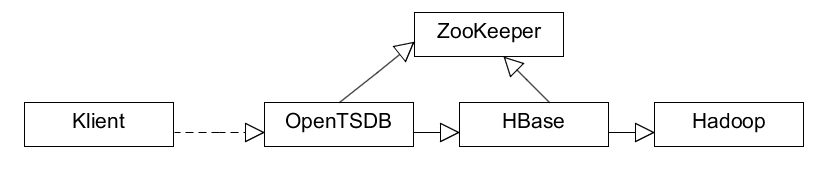
\includegraphics[width=15cm]{opentsdb_architecture}
		\caption[Architektura rozwiązania OpenTSDB]{Architektura rozwiązania OpenTSDB. Klient jest elementem zapisującym dane lub odczytującym je. Strzałki obrazują relację ,,wymaga``.}
		\label{fig:opentsdb_architecture}
	\end{figure}

Rozwiązanie to jest głównie zorientowane na wizualizację danych, dysponując zintegrowanymi rozwiązaniami pozwalającymi na ,,wygładzanie`` brakujących punktów danych. Czasami dokonuje ono manipulacji danymi w celu skutecznego przedstawiania danych w formie graficznej. OpenTSDB na prezentacji danych kładzie nacisk do tego stopnia, że jednym z wymagań przy instalacji jest sprawny pakiet do rysowania wykresów \textit{gnuplot}.

Podobnym rozwiązaniem do OpenTSDB jest projekt, który wyrósł na bazie tegoż, czyli KairosDB. Jest to baza dużo bardziej zorientowana na samo przechowywanie danych niż OpenTSDB, jednak jej zasadniczą cechą jest możliwość korzystania zarówno z HBase, jak i z zalecanego zdecentralizowanego rozwiązania Big Data pod nazwą Cassandra\cite{Lakshman:2010:CDS:1773912.1773922}(reprezentujący identyczny paradygmat bazodanowy jak HBase). W przeciwieństwie do poprzedniego, ze względu na bazę na której się opiera (tj. Cassandra) KairosDB nie ma pojedynczego punktu awarii jakim jest węzeł typu ,,master`` w HBase, ma także lepsze charakterystyki prędkości i skalowalności\cite{cassandra:benchmark}. Widać tutaj, że oba rozwiązania są do siebie podobne, reprezentując nakładki na odpowiednie bazy. Zestawienie to przedstawiono w tabeli \ref{tab:kairos_open}.

\begin{table} \centering \begin{tabular}{|c|c|}
\hline Rozwiązanie & Podstawowa baza danych\\ \hline
KairosDB & Cassandra \\
OpenTSDB & HBase \\
\hline \end{tabular}
\caption{Zestawienie wspomnianych rozwiązań opartych na Big Data} \label{tab:kairos_open} \end{table}

Głównym parametrem przemawiającym za wybraniem któregokolwiek rozwiązania jest posiadanie funkcjonującego klastra jednego z dwóch systemów. Konfiguracja klastra, zarówno HBase jak i Cassandra, jest bowiem nietrywialna\footnote{Choć klaster Cassandra wymaga rząd wielkości mniej czasu do skonfigurowania.}. Zastosowania obu tych baz są tak szerokie, że zwykle przechowywanie szeregów czasowych jest tylko częścią zgromadzonych tam danych.

Pewnym problemem tych baz jest charakter przyjmowania przez nie żądań. Ze względu na to że zostały stworzone w celu zbierania metryk zachowania systemu, a nie pomiarów, nie czynią większych gwarancji na to, że zebrane dane przetrwają. Możliwy jest scenariusz w którym baza otrzyma rozkaz zapisu, potwierdzi go, a awaria następująca 5 sekund potem spowoduje trwałą utratę tych danych. Bierze się to z agresywnego przetrzymywania w pamięci danych, by można było później jednorazowo wpisać większą ilość danych, co zwiększa prędkość działania systemu.

	\subsubsection{Przemysłowe bazy danych typu,,historian``}

Osobną kategorią są rozwiązania tworzone typowo pod problem przechowywania danych pochodzących z pomiarowych systemów na instalacjach automatyki. Znane są one pod nazwą ,,operational historian`` bądź ,,enterprise historian``. Różnicą jest przeznaczenie. ,,Operational historian`` ma docelowo służyć inżynierom monitorującym procesy technologiczne, zaś ,,enterprise historian`` ma zbierać dane do celów procesów biznesowych. Ze względu na coraz większą konwergencję rozwiązań obserwuje się zanik rozróżnień (poza celami marketingowymi). Znaczna większość z nich pozwala na zbieranie danych za pomocą interfejsu OPC HDA\cite{opc:hda}. Rozwiązanie to zostało zbudowane na bazie Microsoft OLE, i jako część standardu OPC stanowi przemysłowy standard w branży SCADA\footnote{czyli systemów zapewniających nadzór i pomiarowanie dla procesów technologicznych}. Tego typu rozwiązania logują również, dla każdego rekordu, wartość ,,jakości próbki``, charakterystyczną w zastosowaniach przemysłowych, gdzie dane mogą być chwilowo niedostępne (np. awaria czujnika) bądź gorszej jakości (inne problemy z czujnikiem). W odróżnieniu od baz typu Big Data, każdy pomiar traktowany jest tutaj jako integralna część szeregu, a utrata większej ilości danych w przypadku awarii jest mniej prawdopodobna.

Dane na temat zasad działania tego typu systemów są wyjątkowo trudno osiągalne. Nie budzi to zdziwienia, ze względu na to, że opracowanie takich systemów wymaga dużych nakładów ze strony firm, a upublicznianie zastosowanych technologii mogłoby podkopać przewagę biznesową firmy. Typową cechą, odróżniającą te rozwiązania od typu Big Data, jest stosowanie wyspecjalizowanych rozwiązań mających na celu ochronę danych przed utratą w razie awarii. Zwykle jest to konfigurowanie systemu do pracy z dużymi redundantnymi macierzami dyskowymi, zamiast korzystanie z wielu tanich komputerów.

Przykładem może być tutaj Proficy Historian firmy GE\cite{proficy:historian}. Rozwiązanie to pozwala dodatkowo na eksport danych do systemów Big Data (Hadoop). Innym rozwiązaniem jest Uniformance PHD\cite{uniformance:phd} firmy Honeywell. Podobnym rozwiązaniem, jednak zorientowanym bardziej na pomiary laboratoryjne jest Citadel\cite{ni:citadel} firmy National Instruments. Mimo bliskiej integracji z środowiskiem LabView dysponuje ono interfejsem OPC. 

Interesującym trendem w przemyśle jest umieszczanie historycznych danych procesowych w chmurze\cite{gecloud}. Jedno z rozszerzeń Proficy Historian umożliwia transfer danych na serwery GE, gdzie mogą być one poddane algorytmom przewidującym czy po prostu składowane.

W ogólności, obserwować można konwergencję rozwiązań ,,historian`` i Big Data. Z odpowiednimi dostosowaniami mogą stanowić rozszerzenia wymienne. Dużą zaletą Big Data jest zdolność do przechowywania również innego charakteru danych i bardzo dobre charakterystyki skalowalności, natomiast główną zaletą rozwiązań ,,historian`` jest obsługa standardów OPC i (czasami) wbudowane algorytmy analityczne. Wewnętrznie bazy ,,historian`` często bardzo przypominają rozwiązania Big Data, co ze względu na restrykcyjne licencje, chroniące rozwiązania przed analizą, ciężko zaobserwować.

	\subsection{Zagadnienia}
Podstawowym problemem baz tego typu jest rozproszenie --- czy to w celu odporności na awarie, czy zwiększenia wydajności. Głównym zagadnieniem jest tutaj koordynacja. Węzły systemu muszą wiedzieć za jakie partie danych odpowiadają, oraz mieć określony sposób reagowania na komendy. W zasadzie wyróżnić tutaj można dwa podejścia
	\begin{itemize}
		\item Z węzłem/węzłami typu ,,master``. Jeden węzeł koordynuje pracę pozostałych. W istotny sposób upraszcza to pracę systemu i zwiększa jego szybkość działania, za cenę wprowadzenia jednak pojedynczego punktu awarii. Problem z jego działaniem w dramatyczny sposób wpływa na działanie całego klastra. Problemy te można do pewnego stopnia zażegnać poprzez wprowadzanie zapasowych węzłów ,,master``, jednak nie eliminują one tego problemu zupełnie. Przykładem jest system HBase.
		\item Bez węzła typu ,,master``. Wszystkie węzły są równorzędne, tak więc eliminuje się pojedynczy punkt awarii. W tym wypadku wymagane są jednak dość złożone algorytmy współpracy i koordynacji aby klaster mógł pracować. Przykładem jest system Cassandra.
	\end{itemize}

Typowe dla systemów o wysokiej niezawodności jest podejście bez węzła ,,master``. Często jednak przewaga prostoty systemu z ,,masterem`` wygrywa, zwłaszcza w systemach, w których analiza ryzyka wykazała że nie jest niezbędna dość wysoka niezawodność. Kolejnym zagadnieniem jest skalowalność. Istnieją dwa podstawowe podejścia do skalowalności, które oczywiście często się ze sobą łączy. Są to:

	\begin{itemize}
		\item Skalowalność pionowa (ang. \textit{scale up}). Tyczy się ona rozszerzania możliwości pojedynczego węzła systemu (większe pamięci, mocniejsze procesory) w celu przetworzenia większych obciążeń. Typowym przykładem takiej skalowalności są systemy typu mainframe. Są to systemy charakteryzujące się dużą wewnętrzną nadmiarowością, dzięki czemu mają wysoką dostępność i odporność na błędy. Dysponują funkcjonalnością która pozwala na rozszerzanie ich w dużym stopniu.
		\item Skalowalność pozioma (ang. \textit{scale out}). Tyczy się ona dodawania kolejnych węzłów do systemu w celu przetworzenia większych obciążeń. Typowym przykładem takiej skalowalności są bazy danych stosowane przez Google czy Facebook - tysiące nieskomplikowanych sprzętowo węzłów typu ARM bądź Intel.
	\end{itemize}

	W zasadzie systemy przetwarzające bardzo duże ilości danych preferują skalowalność poziomą. Istnieją skuteczne algorytmy pozwalające na taki podział danych, aby awaria pojedynczego węzła nie wpłynęła destruktywnie na działanie klastra. Dodatkowo, obecna technologia nie dysponuje możnością stworzenia pojedynczego serwera który mógłby przetwarzać cały zbiór danych. W niektórych przypadkach udaje się przetwarzać duże zasoby danych na pojedynczych węzłach (np. mainframe), jednak ta tematyka wykracza poza zakres tej pracy, chociażby ze względu na wątpliwą stosowalność rozwiązań mainframeowych w przechowywaniu szeregów czasowych. Skalowalność pionowa ma także dużo gorsze parametry niezawodnościowe, gdyż awaria systemu powoduje jego zupełną niedostępność. Wyjątkiem są tutaj systemy redundatne (takie jak mainframe bądź wybrane systemy typu Intel), jednak koszt takich technologii jest znacznie wyższy niż analogiczne przy skalowalności poziomej.

Wymienione tutaj zagadnienia --- charakter rozproszenia i skalowalność --- mają istotne znaczenie w projektowaniu systemu informatycznego, którego zadaniem jest przetwarzanie i przechowywanie dużych ilości danych. Decydują one zarówno o możliwościach (ilościowych) obróbki tychże, a również o charakterystyce niezawodnościowej.

%Kolejny aspekt który przeanalizowano tyczy się konstrukcji samego programu który będzie realizował żądania. Wysokowydajne usługi serwerowe programuje się za pomocą jednego z dwóch sposobów:
%	\begin{itemize}
%		\item Orientacja zdarzeniowa (ang. \textit{event-oriented}), gdzie jeden lub więcej wątków reaguje na przychodzące zdarzenia sekwencyjnie, wykonując krótkie elementy kodu które obsługują te zdarzenia. Wątków jest od jednego do liczby rdzeni serwera. Fundamentalnie działanie takiego serwera opisuje działanie ,,sprawdź co się zdarzyło, a następnie to obsłuż``. Do pobierania informacji o zdarzeniach istnieje szereg intefejsów systemów operacyjnych, zarówno Windows jak i Linux. Ze względów na popularność tego podejścia charateryzuje je dobra wydajność. Systemy oparte na orientacji zdarzeniowej charakteryzuje w praktyce większa wydajność i są one szeroko stosowane w praktyce. 
%		\item Orientacja wątkowa (ang. \textit{threaded}). Tutaj na każde żądanie uruchamiany jest wątek systemu operacyjnego, który sekwencyjnie przetwarza program obsługi danego żądania, zwykle pobierającego rozkaz, wykonującego go i odsyłającego rozkaz. Kod takiego systemu jest znacznie prostszy niż systemu zorientowanego zdarzeniowo, choć wymagana jest synchronizacja. W wielu przypadkach wymaga on także więcej pamięci. Każdy wątek musi dysponować oddzielnym stosem, co przy bardzo dużej liczbie zapytań skutkuje zmarnowaniem dużych ilości pamięci.
%	\end{itemize}

% Rozwój systemów zorientowanych zdarzeniowo przypadał na okres w którym wydajność wątków systemów operacyjnych była stosunkowo niewielka, tak więc wybór takiej architektury nie podlegał większej dyskusji. Obecnie, w obliczu takich rozwiązań jak NPTL (szybkie wątki Linuksa) dopuszczalne są również rozwiązania oparte na wątkach. Z tego powodu, mimo stosowania przez większość rozwiązań orientacji zdarzeniowej, zdecydowano się na opracowanie bazy korzystającej z orientacji wątków.

Istotnym problemem jest również wybór języka programowania. Stanowi on kompromis między prędkością (w ujęciu czasowym) pisania kodu, prostotą jego późniejszego utrzymania i szybkością rozwiązania stworzonego przy użyciu takiego języka. Jeśli chodzi o tworzenie aplikacji serwerowych i bazodanowych, stosuje się języki, które pozwalają na otrzymywanie szybko działających programów, takie jak C, C++, Java i C\# (oraz pokrewne). Rozwój kompilatorów JIT\footnote{Kompilator JIT pozwala przyśpieszyć działanie kodu interpretowanego (stosowanego w Java i C\#) poprzez kompilację ich do kodu maszynowego w trakcie działania programu}. pozwolił na znaczne zminimalizowanie różnic między C/C++ oraz Javą/C\#. W tym momencie istotne stają się także koszty stworzenia takiego rozwiązania oraz późniejszego utrzymywania go. Funkcje takie jak odśmiecacz (ang. \textit{garbage collector}\footnote{Moduł który automatycznie determinuje czy dana zmienna jest wykorzystywana, a jeśli nie --- zwalniający zajmowaną przez nią pamięć}) obecne w nowoczesnych językach programowania pozwalają na przyśpieszenie pracy programisty i minimalizację błędów. Wymienione wyżej języki są najczęściej stosowane do pisania oprogramowania bazodanowego (z drobnymi problemami natury przenośności w przypadku C\#).

Ostatnim już omówionym w tej sekcji zagadnieniem jest replikacja danych. Pod tym pojęciem kryje się przechowywanie identycznych kopii danych na niezależnych węzłach. Jeśli jeden z nich ulegnie awarii, dane wciąż pozostają dostępne w klastrze. Określenie, które węzły w systemie rozproszonym odpowiadają za dane porcje danych, a następnie upewnienie się, że wszystkie dysponują identycznymi zestawami, jest zadaniem złożonym. Jeśli dysponujemy systemem z węzłem ,,master``, to nie stanowi większego problemu rozdzielenie obciążenia między węzły. ,,Master`` może z powodzeniem dokonywać alokacji i informować poszczególne węzły o ich zakresie odpowiedzialności. Problem pojawia się w systemach zdecentralizowanych, gdzie węzły muszą ustalić ten zakres. Ze względu na łatwość użycia i implementacji często stosuje się w tej sytuacji rozwiązania oparte na funkcjach mieszających,  z których jedno opisano w p. \ref{sec:dht}.
	
Większość rozwiązań wykrywających uszkodzenia danych ciągu i decydujących które węzły dysponują danymi właściwymi opiera się na różnego rodzaju sumach kontrolnych. Jednym z rozwiązań są drzewa Merkle'a, w których dane dzieli się na bloki, z których oblicza się sumę kontrolną. Następnie z kilku tych wartości liczona jest kolejna, itd. Obliczenia mogą być wykonywane równolegle ze względu na drzewiasty charakter, dzięki czemu znajdują częste zastosowanie w systemach bazodanowych tego typu. Ideę algorytmu ilustruje rysunek \ref{fig:merkle}. Metoda ta umożliwia szybkie wyliczenie sumy kontrolnej dla danych, a równocześnie, w razie wystąpienia różnic, określenia której części danych dotyczy problem (porównanie wartości sum kontrolnych ,,niższego poziomu''). 

	\begin{figure}[h]
		\centering 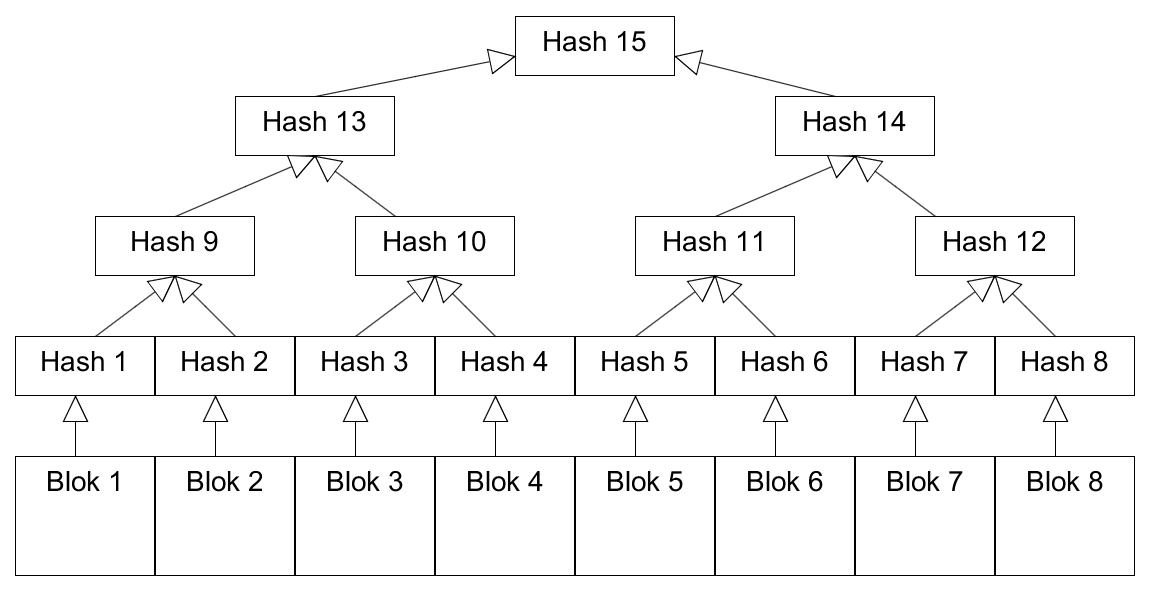
\includegraphics[width=15cm]{merkle}
		\caption{Ilustracja metody drzew Merkle'a}
		\label{fig:merkle}
	\end{figure}

W przypadku danych szeregów czasowych, gdzie zazwyczaj dane zapisane w blokach ,,przeszłości`` nie będą już modyfikowane, przypadek drzew Merkle'a można zdegenerować do łańcucha liczącego sumę kontrolną na podstawie własnych danych i sumy kontrolnej poprzedniego węzła. Podejście to jednak nie jest do zastosowania w systemach umożliwiających modyfikację przeszłych danych, chociażby takich jak zgodne z OPC HDA.

Możliwe są oczywiście inne metody sprawdzania spójności ciągu. W projektowanym nowym rozwiązaniu zdecydowano się na nowatorską metodę. Polega ona na wymaganiu podania, przy poleceniu dopisania nowego rekordu, stempla czasowego poprzedniego rekordu. Element zapisujący dysponuje tą informacją, zaś węzeł na tej podstawie może stwierdzić czy zarejestrował cały przebieg, czy niektórych elementów mu brakuje. Tak czy inaczej, powinien przyjąć zapis - pozostałe przecież nie mogą czekać. Schemat blokowy ilustrujący tą ideę przedstawiono na rysunku \ref{fig:novel_decider}.

	\begin{figure}[h]
		\centering 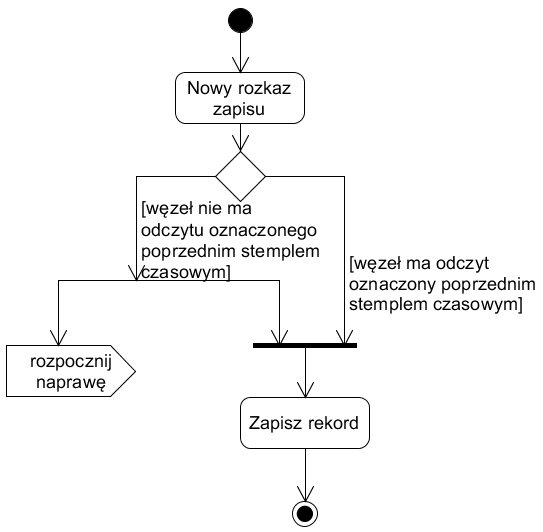
\includegraphics[width=11cm]{novel_decider}
		\caption{Schemat blokowy nowej metody sprawdzania spójności}
		\label{fig:novel_decider}
	\end{figure}

	\subsection{Rozproszona tabela mieszająca}
	\label{sec:dht}
Algorytm rozproszonej tabeli mieszającej (ang. DHT) jest popularnym sposobem przyporządkowania danych do konkretnych węzłów oraz odszukiwania tych informacji, stosowanych w rozproszonych systemach bazodanowych.

Fundamentalnie zakłada on abstrakcję tablicy asocjacyjnej, czyli zbioru dwuelementowych krotek \textit{(klucz,wartość)}, gdzie klucz najczęściej będzie ciągiem znaków. Aby zastosować teraz tabelę mieszającą, wymagane jest obliczenie dodatkowo funkcji mieszającej. Funkcja taka przyporządkowuje ciągowi bajtów wartość z pewnego skończonego zakresu w ten sposób że histogram jej zbioru wartości jest ,,płaski``\footnote{w praktyce oznacza to że dla dużej próbki danych wejściowych zaobserwuje się równomierną częstość występowania wartości wynikowych}. Ponieważ zbiór wartości klucza jest zbiorem nieskończonym, stosujemy funkcję, która przyporządkuje mu wartość ze zbioru skończonego. Funkcja ta z konieczności musi być funkcją nieodwracalną.

Idea tabeli mieszającej polega na rozdzieleniu między węzły zakresów wartości tej funkcji, dzięki czemu na podstawie klucza ustalić można który węzeł jest zań odpowiedzialny. W praktycznych implementacjach rozproszonych tabel mieszających pojedynczy węzeł nie posiada informacji o wszystkich innych komponentach systemu, a jedynie o niektórych. Każde zapytanie o dany klucz może więc skończyć się dwojako – albo potwierdzeniem, że to właśnie odpytywany węzeł zań odpowiada, albo wskazaniem na inny węzeł, który może mieć tę informację. Przykładem może być tutaj rozwiązanie mapujące znane jako Chord \cite{Stoica:2001:CSP:383059.383071}, w którym jeden węzeł przechowuje informację tylko o ok. $O(log N)$ węzłach. Powoduje to że z wysokim prawdopodobieństwem ustalenie węzła następuje w ciągu nie więcej niż $O(log^2 N)$ wiadomości wymienionych ze składnikami klastra. Istnieją również systemy, w których węzły przechowują informację o wszystkich innych węzłach w klastrze (np. Cassandra \cite{Lakshman:2010:CDS:1773912.1773922}).

	\begin{figure}[h]
		\centering 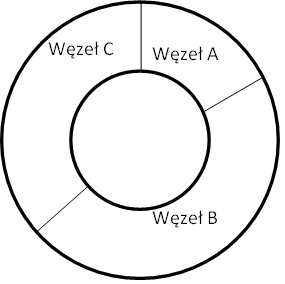
\includegraphics{sch_ide_token_ring}
		\caption{Schemat ideowy przykładowego podziału przestrzeni wartości funkcji mieszającej na trzy węzły}
		\label{fig:sch_ide_token_ring}
	\end{figure}

W przypadku systemów w których na jednym węźle dostępna jest pełna informacja o innych węzłach lokalizacja danych zostanie znaleziona najwyżej w 2 zapytaniach. W takim wypadku węzły odpowiedzialne są za przedziały zbioru wartości funkcji mieszającej i tworzą logiczną topologię pierścienia, działającej zgodnie z zasadami arytmetyki modularnej. W tym momencie do stworzenia pełnego obrazu wystarczy, żeby węzłowi przyporządkować wartość początkową przedziału za który jest on odpowiedzialny. Na rysunku \ref{fig:sch_ide_token_ring} został pokazany schemat topologii pierścienia o trzech węzłach. Dodatkową elastycznością takiego rozwiązania jest to, że mocniejszym sprzętowo węzłom można delegować większe zakresy, dzięki czemu możliwe jest zastosowanie takiego rozwiązania w systemach heterogenicznych. Systemem heterogenicznym nazwiemy klaster, w którym węzły nie są identyczne, w szczególności dysponują sprzętem o różnej mocy przerobowej oraz czasami innymi systemami operacyjnymi.

	\docsection{Charakterystyka systemu}
W rozdziale opisano system kontrolno-pomiarowy, dla którego buduje się rozwiązanie bazodanowe, oraz powody, dla których zdecydowano się na stworzenie nowego rozwiązania. Podano, jak wygląda przepływ danych wewnątrz systemu kontrolno-pomiarowego, oraz analizę, mającą na celu ustalenie ilości danych, z którymi system będzie miał do czynienia. Przedstawiono dalej ogólny charakter tworzonego rozwiązania wraz z jego założeniami, oraz przegląd komponentów systemu. Na końcu przedstawiono właściwości \textit{ciągu}, jako podstawowego elementu projektowanej bazy danych.

\subsection{System kontrolno-pomiarowy}

Tworzone rozwiązanie znajdzie zastosowane w rozproszonych systemie kontrolno-pomiarowym, jakim jest funkcjonujący na rynku od 6 lat \textbf{smok-serwis.pl}. SMOK\cite{smok} jest tutaj akronimem od ,,system monitoringu odległych kotłowni``, co jednocześnie jest jego podstawowym zadaniem. System ten zbiera dane z kilkuset instalacji grzewczych, zarówno klasycznych kotłowni gazowych jak i węzłów ciepłych, czy nawet instalacji solarnych, oraz przetwarza te dane, generując powiadomienia o awariach i raporty dotyczące możliwości optymalizacji. Ze względu na ilość zbieranych danych, oraz konieczności zapewnienia nieprzerwanej pracy, nawet w warunkach awarii części infrastruktury serwerowej projektowany system będzie spełniał swoje zadania.

Istotny jest tu warunek poprawnej pracy systemu nawet w przypadku awarii części systemu serwerowego. System w trybie ciągłym musi nadzorować monitorowane obiekty, oraz być w stanie wysłać powiadomienia w wypadku awarii jednego z nich do odpowiednich służb serwisowych. Aby osiągnąć ten cel wymagana jest sprawność podsystemu bazodanowego, co stanowi motywację dla takiego wymagania.

Fundamentalnie SMOK składa się z wielu oddzielnych lub luźno związanych (np. ze sobą obiektów grzewczych (np. węzłów grzewczych na tej samej linii MPEC\footnote{Miejskie Przedsiębiorstwo Energetyki Cieplnej --- funkcjonująca w wielu miastach nazwa lokalnej firmy, będącej zazwyczaj własnością miasta, zajmującej się dostarczaniem energii cieplnej do budynków w postaci ciepłej wody. Ciepła woda ta następnie wykorzystywana jego do ogrzewania budynku za pomocą instalacji ciepłego ogrzewania.}), raportujących stan swoich czujników i parametrów do systemu za pomocą modułu dostępu. Medium, za pomocą którego to czyni może być sieć GSM lub lokalne łącze internetowe (Ethernet, WiFi). Moduł dostępu przesyła dane w czasie rzeczywistym do serwerowego systemu obsługi i kontroli, który po ewentualnej obróbce umieszcza dane w bazie systemu kontrolno-pomiarowego. Baza ta następnie służy do prowadzenia analizy i rysowania wykresów. Ideowy schemat architektury systemu SMOK przedstawiono na rysunku \ref{fig:smok_architecture}.

	\begin{figure}[h]
		\centering 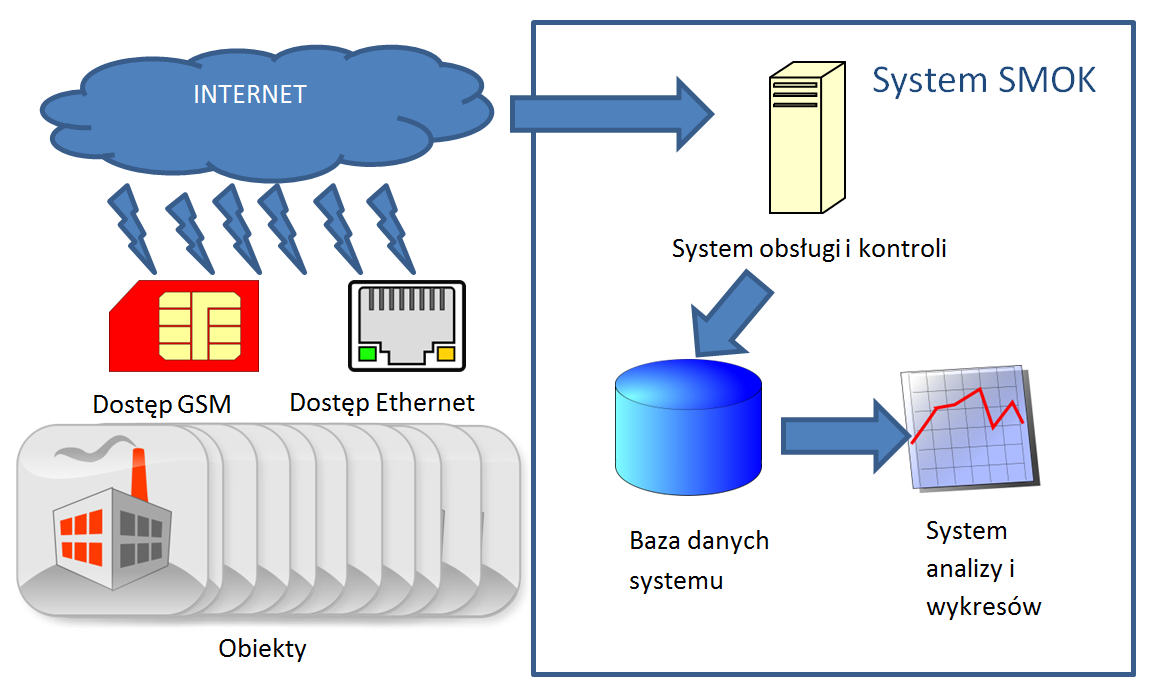
\includegraphics[width=15cm]{smok_architecture}
		\caption{Schematyczna architektura systemu SMOK}
		\label{fig:smok_architecture}
	\end{figure}

Mimo że na rynku dostępnych jest szereg rozwiązań bazodanowych, zarówno typu ,,historian`` jak i rodzaju ,,Big Data``, zdecydowano się na stworzenie nowego rozwiązania. Przemawia za tym szereg powodów:
	\begin{enumerate}
		\item Obecne rozwiązania typu Big Data cechuje wysoki poziom trudności przy wdrożeniu. Wymagają one instalacji dużej ilości oprogramowania ze względu na rozległe wymagania elementów.
		\item Bazy typu ,,historian``, przystosowane do zbierania danych przemysłowych w sposób ideowo zgodny z zasadami branży, są rozwiązaniami płatnymi. Nowe rozwiązanie planuje się jako otwarte oprogramowanie.
		\item Nowe rozwiązanie stosuje nowatorską metodę sprawdzania spójności ciągu, której działanie i przydatność warto zweryfikować. 
%		\item Chęć sprawdzenia podejścia orientacji wątkowej przy obsłudze dużych ilości danych na nowoczesnym systemie operacyjnym.
		\item Implementacja wydanej funkcji automatycznego kasowania danych starszych niż zadana wartość jako elementu polityki retencji danych.
		\item Elementarnie prosty sposób przechowywania danych pozwala uprościć procedurę odzyskiwania danych w przypadku masowej awarii węzłów.
		\item Silna gwarancja przetrwania danych --- w momencie gdy baza potwierdzi zapis, dane na pewno nie ulegną utracie w przypadku awarii.
		\item Stosowalność i dobry charakter pracy w zaprezentowanym systemie SMOK.
		\item Możliwość sprawowania kontroli nad kodem źródłowym i prawami majątkowymi rozwiązania ze względu na brak obciążeń licencyjnych.
		\item Zbyt mała ilość danych by angażować typowe rozwiązania Big Data.
		\item Zależność innych rozwiązań od dużej ilości innych bibliotek i rozwiązań programowych. Obecność dodatkowych usług i programów może zwiększać podatność na włamania systemu informatycznego.
	\end{enumerate}

Podstawowym problemem rozwiązywanym w tej pracy było stworzenie programu --- bazy danych. Baza ta ma służyć do przechowywania szeregów pomiarowych. Szereg pomiarowy stanowi zbiór odczytów opatrzonych stemplem czasowym wykonania takiego pomiaru. Jego najprostszą wizualizacją jest wykres obrazujący zmiany parametru w czasie. Szeregi pomiarowe są istotnym rodzajem danych dla systemów kontrolno-pomiarowych.

Baza ta będzie umożliwiała dopisanie do danego ciągu\footnote{pojęcie stosowane w pracy oznaczające szereg pomiarowy} wykonanego pomiaru wraz z jego stemplem czasowym. Będzie możliwe również pobranie historii danego punktu pomiarowego - zarejestrowanych dlań pomiarów wraz z czasami ich zdjęcia. Charakter takich danych najłatwiej przedstawić na wykresie. Przykładowy wykres zaprezentowano na rysunku \ref{fig:sample_plot}.

	\begin{figure}[h]
		\centering 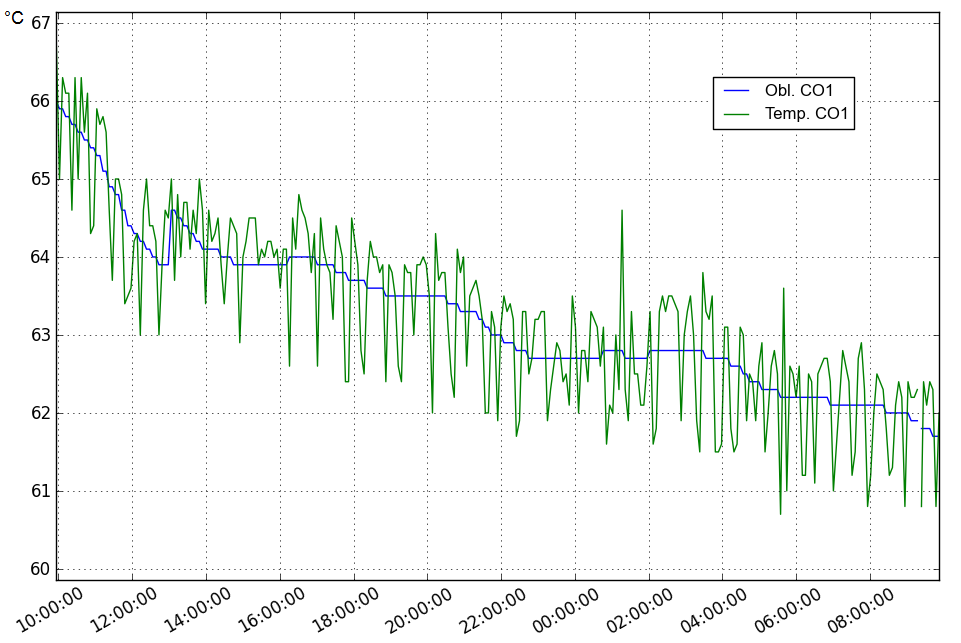
\includegraphics[width=15cm]{sample_plot}
		\caption[Przykładowy wykres danych, które mogą być zbierane przez stworzoną bazę]{Przykładowy wykres danych, które mogą być zbierane przez stworzoną bazę. Na wykresie przedstawiono dwa szeregi pokazujące przebieg temperatury w czasie.}
		\label{fig:sample_plot}
	\end{figure}
Rozwiązanie zamierzono jako rozproszoną bazę danych. Podstawową racją rozproszenia jej jest odporność na awarie pojedynczych węzłów wchodzących w skład klastra bazy oraz skalowalność --- to znaczy możliwość obsługi większej ilości danych i połączeń równocześnie niż to możliwe na pojedynczym węźle. W przypadku naprawienia awarii danego węzła i ponownego włączenia go do klastra, węzeł ten powinien zsynchronizować swój stan z resztą, to jest pobrać brakujące dane, które ,,ominęły`` go w trakcie gdy nie był w klastrze.

Równocześnie, ze względu na wydajność i tolerancję na awarie, zdecydowano, że w systemie nie będzie węzła typu \textit{master}, który w jakiś sposób mógłby koordynować działania podległych mu węzłów. Ma to istotny wpływ zarówno na projekt bazy, jak i na jej właściwości.

\subsection{Przepływ danych}

Analizując potrzeby bazodanowe systemu SMOK należy spojrzeć na to, w jaki sposób dane będą przepływać przez system. Należy dokonać takiej analizy zarówno w aspekcie pozyskiwania, jak i odczytywania tych danych. Źródłem informacji są obiekty monitorowane przez system, które definiują listę mierzonych czujników (np. temperatury, ciśnienia). Mierzą one interesujące operatora wartości, takie jak temperatura kotła, temperatura zewnętrzna czy temperatura wody w sieci. Konsumentami informacji natomiast są komponenty optymalizujące pracę kotłowni, generujące raporty, detektory błędów czy interfejs użytkownika Web.

\begin{figure}[h]
	\centering 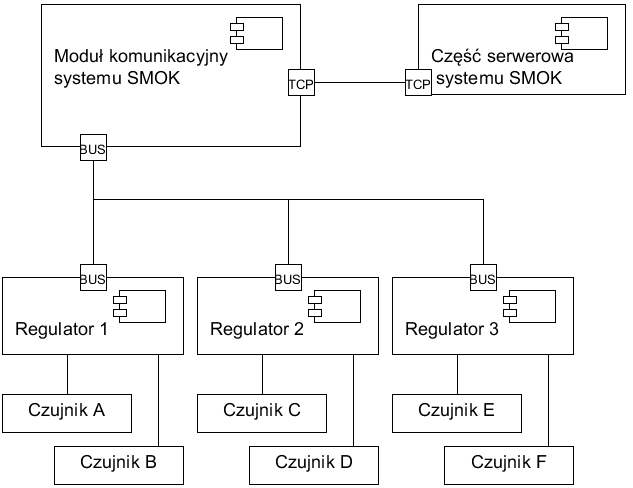
\includegraphics[width=10cm]{smokarc_clientsite}
	\caption{Schemat komunikacji w miejscu instalacji modułu}
	\label{fig:smokarc_clientsite}
\end{figure}

Miejscem najbliższym sensorom mierzącym parametry jest obiekt na którym zainstalowano system. Do regulatorów, zawiadujących pracą urządzeń wykonawczych, podłączone są czujniki. Charakter tego połączenia, z punktu widzenia serwerowej części systemu, jest nieistotny, gdyż system nie prowadzi komunikacji bezpośrednio z nimi. Moduł ten, stanowiący most między serwerową częścią systemu SMOK a automatyką w miejscu instalacji, koordynuje proces odpytywania konkretnych regulatorów. Dzięki temu moduł komunikacyjny z punktu widzenia serwerowej części systemu stanowi warstwę abstrakcji dla regulatorów i czujników. Ideowy schemat instalacji systemu na obiekcie grzewczym przedstawiono na rysunku \ref{fig:smokarc_clientsite}. Regulatory, zamontowane na obiekcie, są w stanie pracować bez udziału modułu komunikacyjnego. Aby uzyskać odczyt z danego czujnika moduł musi wystosować zapytanie do regulatora. Zapytania takie realizuje moduł na polecenie serwera, z którym łączy się za pomocą protokołu TCP.

Moduł komunikacyjny pracuje w stosunku do serwera w konfiguracji master-slave, realizując rozkazy w reżimie synchronicznym\footnote{tj. pytanie-odpowiedź}. Kolejnym etapem jest rozpatrzenie przepływu informacji wewnątrz systemu serwerowego i jej relacji do systemu bazodanowego. Schemat ideowy przepływu zaprezentowano na rysunku \ref{fig:smokarc_serversite}.

\begin{figure}[h]
	\centering 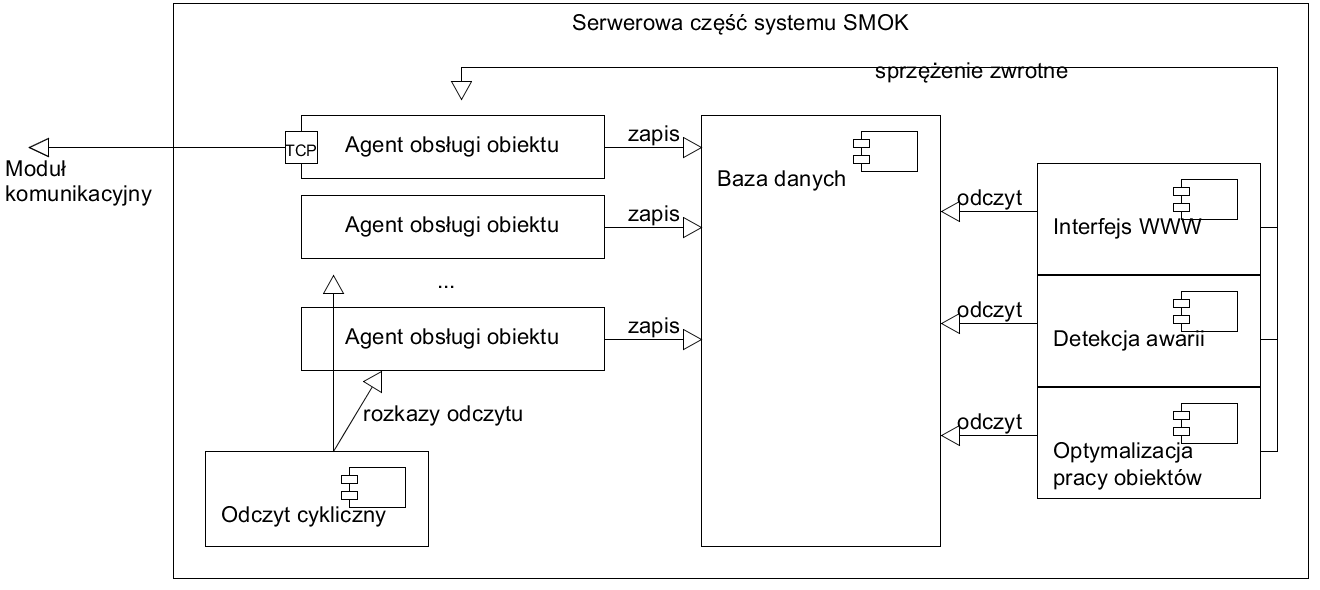
\includegraphics[width=15cm]{smokarc_serversite}
	\caption{Schemat przepływu danych wewnątrz części serwerowej}
	\label{fig:smokarc_serversite}
\end{figure}

Moduł komunikacyjny systemu SMOK łączy się za pomocą połączenia TCP z odpowiednim dla obiektu tzw. agentem obsługi obiektu. Jest to proces działający na systemie serwerowym SMOK. Dla każdego zdefiniowanego w systemie obiektu działa odpowiedni agent. Ze względu na ilość agentów, istotne jest zarządzanie obciążeniem systemu. Agenty bowiem działają równolegle i w izolacji od siebie nawzajem, tak więc nie synchronizują między sobą swoich działań. Nad tą kwestią czuwają nad tym odpowiednie podsystemy które w dynamiczny sposób równoważą obciążenie między węzłami systemu serwerowego, co pozwala systemowi SMOK skalować się liniowo.

Agent obsługi obiektu spełnia dwojaką funkcję. Pierwszą z nich jest odbieranie poleceń odczytu parametrów i modyfikacji parametrów od różnych komponentów systemu. Mogą być to zarówno elementy korzystające z danych, wysyłając takie rozkazy w ramach sprzężenia zwrotnego.  Innym elementem, którego jedynym zadaniem jest wysyłanie rozkazów odczytu, jest komponent ,,Odczyt cykliczny``, który co minutę wymusza odczyt wartości. Robi to, by zapewnić że odczyty realizowane będą w wymaganych odstępach, tj. co minutę. Agent, oprócz poleceń odczytu, otrzymuje też rozkazy zmiany parametrów regulacyjnych na urządzeniu. Dzieje się to zwykle po interwencji użytkownika, choć może być też wykonywane automatycznie poprzez zmiany zaplanowane czy automatyczną optymalizację pracy obiektu.

Drugą funkcją agenta jest wysyłanie poleceń do modułu komunikacyjnego za pomocą połączenia TCP w odpowiednim formacie, oraz koordynowanie ich wykonywania. Odczyty i zapisy wartości agent realizuje szeregowo, w takim formacie bowiem przyjmuje je moduł komunikacyjny. Wykonanie serii odczytów zajmuje pewien czas. Ponieważ system odczytuje parametry co minutę, czas trwania serii odczytów musi być mniejszy od minuty. W praktyce jest on zupełnie wystarczający, nawet na odczytanie kompletnego zestawu pomiarów z bardzo dużych instalacji\footnote{rzędu czterech kotłów gazowych, dziesięciu obiegów centralnego ogrzewania i trzech zasobników ciepłej wody}.

	\begin{figure}[h]
		\centering 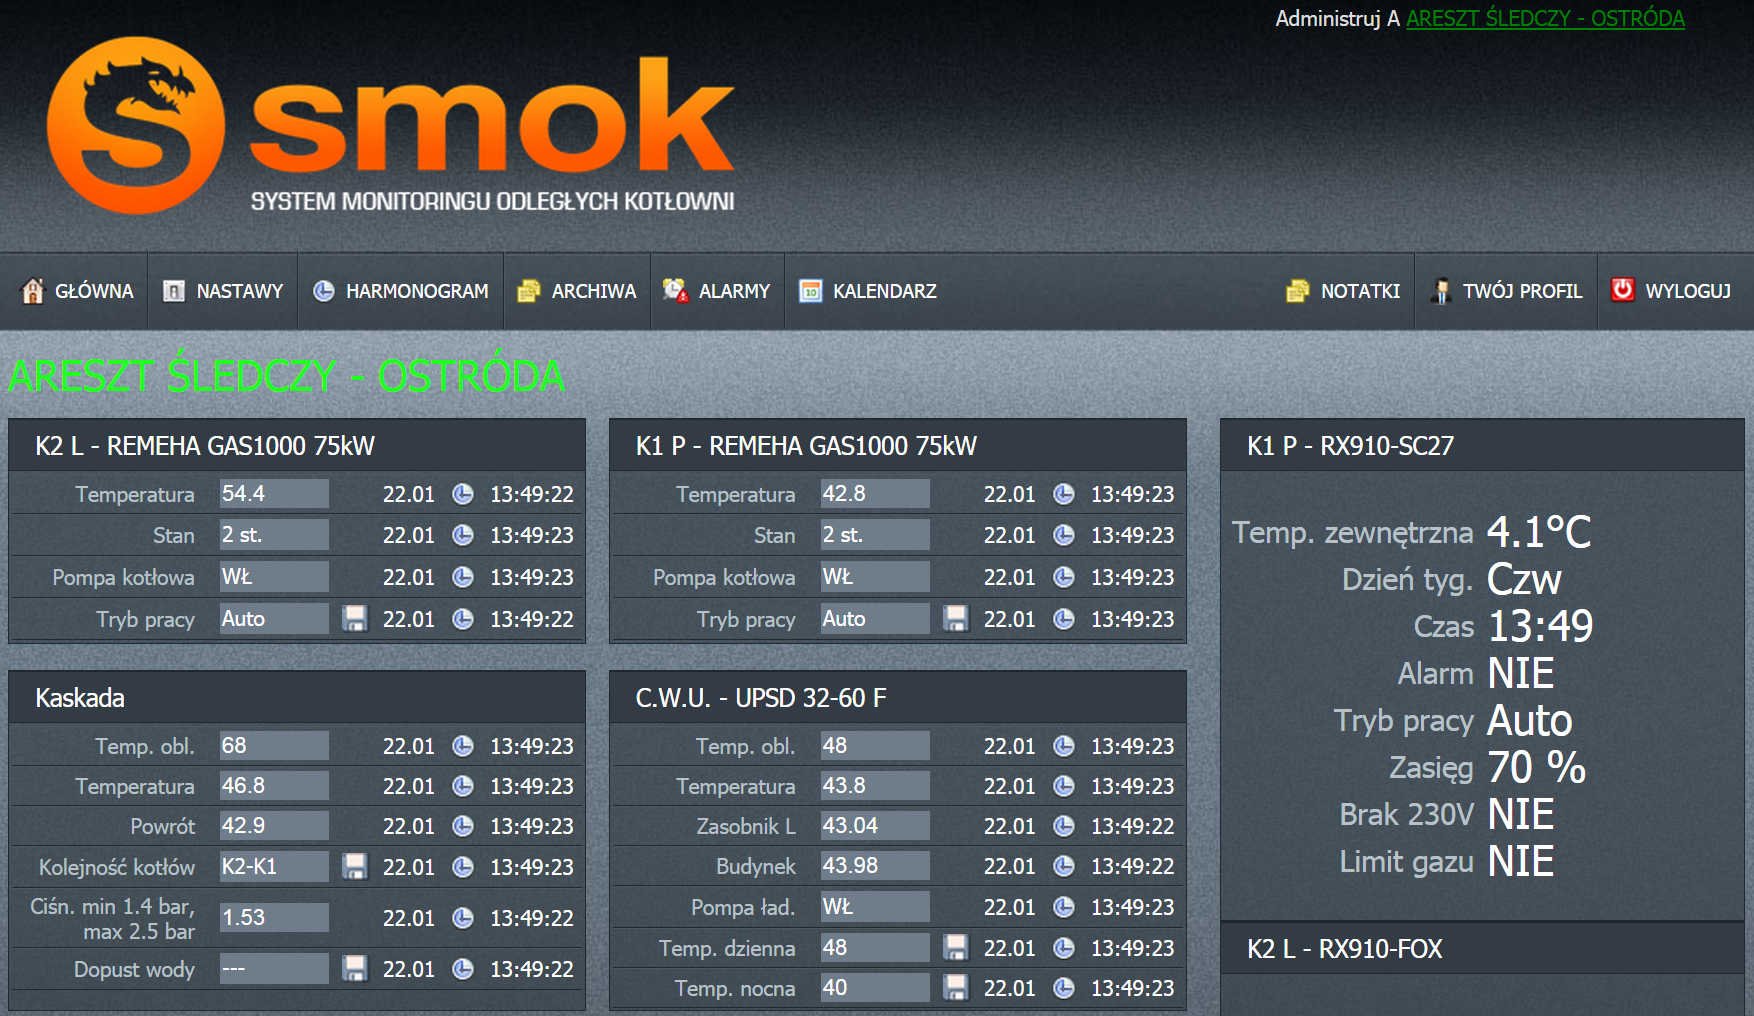
\includegraphics[width=15cm]{smokscreenshot}
		\caption{Zrzut ekranu interfejsu WWW z produkcyjnej wersji systemu SMOK}
		\label{fig:smokscreenshot}
	\end{figure}

Agent po otrzymaniu wartości parametru od modułu komunikacyjnego umieszcza go w bazie danych. Odpowiada on za wszystkie ciągi wartości pomiarowych danego obiektu i jest jedynym elementem w systemie który będzie do tych ciągów dopisywał nowe dane. Z danych tych później korzystają inne elementy systemu. Największymi konsumentami tych danych są trzy podzespoły uwidocznione na rysunku \ref{fig:smokarc_serversite}. Są to:
\begin{itemize}
	\item interfejs WWW --- zapewnia dostęp do informacji odnośnie stanu obiektu przez WWW. Pozwala użytkownikowi przeglądać aktualny stan, uzyskiwać dostęp do wykresów obrazujących jego pracę oraz pozwala zmieniać parametry regulacyjne. Przykładowy zrzut ekranu z produkcyjnej wersji systemu przedstawiono na rys. \ref{fig:smokscreenshot},
	\item detekcja awarii --- jest to podzespół który niezależnie od kontroli obiektów przez użytkowników wykrywa czy parametry pracy nie świadczą o problemach regulacyjnych bądź awarii elementów wykonawczych. Po stwierdzeniu awarii informuje on użytkownika o problemie,
	\item optymalizacja pracy obiektów --- podzespół ten analizuje pracę obiektu i jest w stanie interweniować w przypadku wykrycia sytuacji w której automatyka reguluje układem w sposób nieoptymalny ze względu na źle dobrane parametry regulacji (np. nastawy regulatorów PID).
\end{itemize}

Agent obsługi obiektu dopisuje do bazy, wartości pomiarów zaraz po ich odebraniu, które z drobnymi odstępami czasowymi odbiera szeregowo. Interfejs WWW odczytuje najczęściej ostatnią dopisaną wartość do danego ciągu, czasami całe zakresy czasowe danych w przypadku konieczności stworzenia wykresu. Pozostałe podzespoły odczytują całe zakresy czasowe. Ze względu na możliwość prowadzenia różnych przekształceń przez agenta, polecenia odczytu kierowane do agenta są tylko asynchroniczne. Przechodzą one dość długą drogę, co ilustruje diagram UML sekwencji na rysunku \ref{fig:smokarc_seqdg}. Agent przed wykonaniem otrzymanego polecenia może wykonywać również inne operacje, co decyduje o asynchroniczności części operacji.

\begin{figure}[h]
	\centering 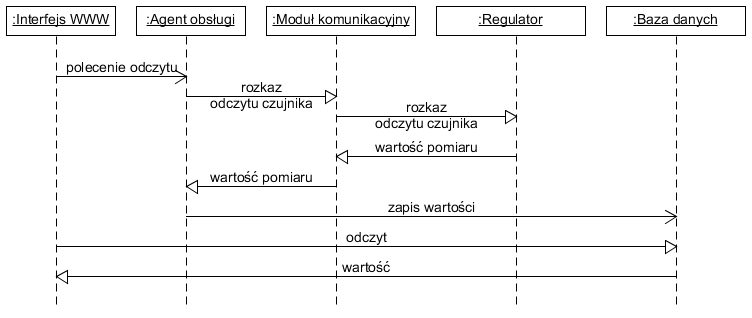
\includegraphics[width=15cm]{smokarc_seqdg}
	\caption{Schemat sekwencji odczytu pojedynczego parametru}
	\label{fig:smokarc_seqdg}
\end{figure}

Powyższe przedstawienie przepływu danych wewnątrz systemu kontrolno-pomiarowego, z którym ma być sprzężona projektowana baza danych, uwidacznia charakter operacji przeprowadzanych na tej bazie. Dodatkowo pokazuje dlaczego stabilne i pewne działanie bazy jest konieczne dla pracy systemu.

\subsection{Analiza ilości danych}
\label{sec:data_quantity_analysis}
Aby system mógł wywiązywać się z tych zadań, musi przechowywać i przetwarzać szeregi czasowe. Są to parametry z podłączonych kotłowni, takie jak stan urządzeń wykonawczych, temperatury, ciśnienia czy natężenia prądów. W przypadku komunikacji GSM przechowywana jest także informacja o jakości połączenia. Prezentowana w tej pracy baza danych będzie stanowić podsystem odpowiedzialny właśnie za to. Aby przedstawić konkretny plan, niezbędna jest najpierw analiza wolumenu danych, które system przetwarza obecnie, oraz prognozy wzrostu.

Wg stanu na 18 grudnia 2014, SMOK monitoruje 512 obiektów. Każdy z nich ma średnio 14 punktów pomiarowych, z których dane muszą być archiwizowane bezterminowo, oraz około 98 punktów, które mogą być przechowywane tylko przez krótki okres\footnote{Dużą część z nich stanowią parametry regulacyjne, które nie w każdym cyklu są odczytywane. Inne odczyty nie są tak ważne by archiwizować je bezterminowo, jednak są przydatne operatorowi nadzorującemu pracę obiektu po zalogowaniu do systemu.}. Istnieją również dodatkowe informacje na temat obiektów, jednak nie są one interesujące z punktu widzenia analizy ilości zebranych danych.
\begin{align*}
	512 * 14 = 7168	\\
	512 * 98 = 50176
\end{align*}	

Sumarycznie daje to 7168 punktów przechowujących dane bezterminowo i 50180 punktów o krótkim przechowywaniu danych. Każdy z nich wymaga maksymalnie 4 bajtów na opisanie wartości, opowiadającej zmiennej typu \textit{float}. Po doliczeniu stempla czasowego, jeden rekord będzie miał 12 bajtów. Pomiary przechowywane bezterminowo generowane są co jedną minutę. W przypadku pomiarów o przechowywaniu terminowym będzie to około 15 sekund, ale przy przechowywaniu jest to nieistotne na dłuższą metę, gdyż zgodnie z założeniami ma być przechowywane maksymalnie 15 minut. 

Zapis co minutę jest z punktu widzenia analizowanych zjawisk wystarczający. SMOK zajmuje się zagadnieniami ogrzewania. Procesy cieplne są procesami wolnozmiennymi. Zjawiska okresowe, mogące być interesujące z punktu widzenia analizy, mają okres właściwie zawsze większy od 2 minut, co spełnia warunek Nyquista. Patologicznymi zjawiskami okresowymi są np. oscylacje temperaturowe, świadczące o błędnej regulacji układu. W procesach inercyjnych, jakimi są procesy temperaturowe, są to procesy wolnozmienne. Zbieranie wartości co minutę w zupełności wystarcza, aby zarejestrować i zidentyfikować takie przypadki. Ponadto doświadczenie z ponad pięcioletniej eksploatacji systemu dodatkowo upewnia w słuszności powziętego założenia.

Tak więc ciągi generowane przez punkty o przechowywaniu terminowym zajmą maksymalnie 35 MB\footnote{$50180 \times 12 b \times 4 min^{-1} \times 15 min$}. Ciągi o przechowywaniu bezterminowym generują ok. 84 kB\footnote{$7168 \times 12b$}danych na minutę, co tłumaczy się na 120 MB dziennie, czyli 42,8 GB rocznie\footnote{jest to wartość mniej więcej zgodna z rzeczywistością, danych tych jest nieco mniej ze względu na awarie poszczególnych urządzeń}.  Tak więc --- ze względu na takie porównanie --- w dalszej analizie można zaniedbać rozpatrywanie ciągów o przechowywaniu terminowym. Wg zgłoszonego przez operatora stanu na 18 grudnia 2014, system zgromadził 48 GB danych dla 512 urządzeń.

System ulega ciągłej rozbudowie. Statystyki udostępnione przez operatora systemu wskazują, że jedno urządzenie dostępowe, obsługujące nowy obiekt grzewczy, montowane jest średnio co 3 dni. Wykonano dodatkowo prognozy dla montowania urządzenia co 2\footnote{Wg operatora systemu występowały przypadki montażu nawet 20 urządzeń dziennie.} oraz co 5 dni. Są to wartości odpowiednio uśrednione, użyteczne dla zastosowań modelowania i prognozy.

Jako okres obliczania można więc przyjąć $x$ dni. Tak więc, ilość danych zgromadzonych w ciągu takiego okresu wynosić będzie 
\begin{align*}
	x(14 \times 12B \times 4 min^{-1} \times 60 \frac{min}{h} \times 24 h) = x \times 80640 B
\end{align*}

Mając początkową wartość 48 GB w okresie ,,startowym`` $o_{0}$ ilość danych dla następnego okresu obliczyć można:
\begin{align*}
	o_{a+1} = o_a + x \times p \times 80640 B
\end{align*}

Gdzie $p$ to liczba urządzeń. Oczywiście, będzie się ona zwiększać co okres rozliczeniowy. Mając początkową liczbę urządzeń równą 512 oznaczoną $p_{0}$ można zapisać:
\begin{align*}
	o_{a+1} = o_a + (p_{0} + a) \times x \times 80640 B
\end{align*}

	\begin{figure}[h]
		\centering 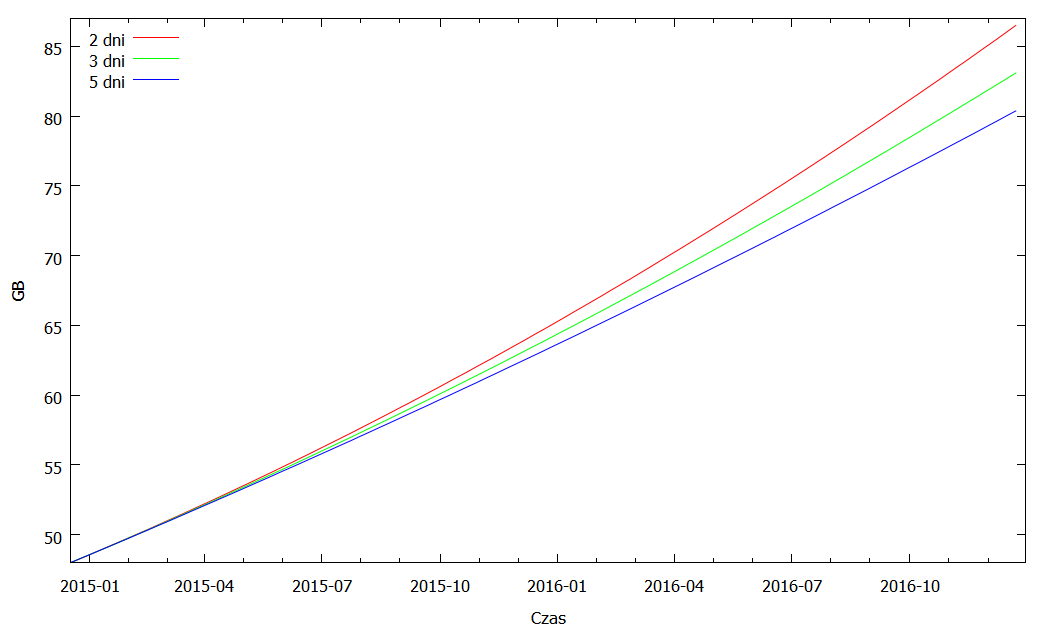
\includegraphics[width=15cm]{smok_prognosis}
		\caption[Prognoza ilości danych zgromadzonych w systemie na lata 2015, 2016]{Prognoza ilości danych zgromadzonych w systemie na lata 2015, 2016 wykonana za pomocą modelu dla trzech różnych odstępów między dodaniem nowego urządzenia do systemu.}
		\label{fig:smok_prognosis}
	\end{figure}

Wykonaną za pomocą tego modelu prognozę na rok 2015 i 2016 ujęto w wykresie na rysunku \ref{fig:smok_prognosis}. Jest to oczywiście tylko prognoza, nieuwzględniająca zmienności warunków rynkowych. Na koniec roku 2016 przewiduje się rozmiar danych najwyżej 87 GB. Przy założeniu podwójnej replikacji danych będzie to zajmować 174 GB danych. Stworzona baza danych przeszła integrację na testowej platformie systemu, zaś jej szersze wdrożenie planowane jest na wiosnę 2015.
 
Aby dokładniej określić wymagania systemu, należy ustalić maksymalne planowane obciążenia systemu. W tym przypadku, biorąc pod uwagę odpowiednio duży zapas, zdecydowano się na ustalenie tej wartości jako model 2-dniowy\footnote{to jest, przy założeniu dodawania jednego obiektu co w dni} dla roku 2025. Jest to 2345 urządzeń oraz 442 GB zgromadzonych danych, co dla podwójnej replikacji daje 884 GB danych. Planując cztery węzły, na każdym wymagane jest przynajmniej 221 GB na ten cel. Daje się to zrealizować na typowych dyskach 500 GB czy nawet 250 GB. Nie muszą być to systemy RAID, ze względu na redundancję systemu.

\subsection{Założenia i zarys działania}
		\label{sec:assumptions}
Pierwszym założeniem, które należy poczynić przy projektowaniu jakiejkolwiek bazy danych jest charakter przechowywanych danych. Projektując bazę systemu kontrolno-pomiarowego wiadomo że będą to dane pomiarowe, czyli zbiór uporządkowany wartości opatrzonych informacją o jakości próbki i czasie jej pobrania. W bazie występować może wiele takich ciągów, z których każdemu, w celu identyfikacji, nadać należy nazwę.

Oczywiste również jest że wartość stempla czasowego będzie stale rosnąć. Istnieje zależność polegającą na tym, że w ramach danego przyporządkowania – dalej nazywanego ciągiem – wartość stempla będzie rosnąca. Niemożliwe będzie dodanie do danego ciągu próbki starszej niż najmłodsza w nim obecna. W znaczący sposób ułatwi to później przeszukiwanie i zarządzanie danymi.

Dodatkowo każda próbka, którą wraz ze stemplem czasowym nazwać można rekordem, będzie miała taką samą długość. Systemy pomiarowe z reguły generują dane o równej długości, najczęściej będące właśnie krotką stempla czasowego, wartości zmierzonej i informacji o jakości próbki. Nadanie im równych długości w ramach konkretnego ciągu pozwoli na istotne uproszczenie i przyśpieszenie działania systemu. Przykład takiego ciągu zamieszczono na rysunku \ref{fig:a_series}.

	\begin{figure}[h]
		\centering 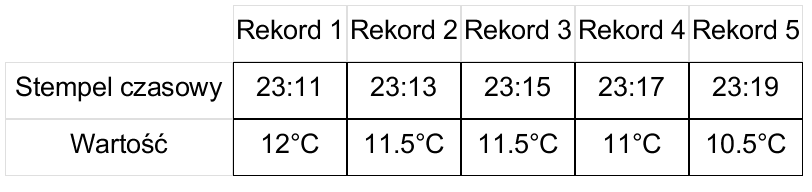
\includegraphics[width=12cm]{a_series}
		\caption[Przykład ciągu o 5 rekordach z rosnącym stemplem czasowym]{Przykład ciągu o 5 rekordach z rosnącym stemplem czasowym. Ze względu na czytelność datę pominięto.}
		\label{fig:a_series}
	\end{figure}

Reasumując, możliwymi operacjami do wykonania na ciągu muszą być przynajmniej odczyt, dopisanie nowego rekordu i skasowanie całego ciągu. Jeśli wymagać tylko tych operacji, to takie ograniczenie pozwoli w dalszym rozrachunku na uproszczenie programu i jest zupełnie wystarczające dla celów bazy danych systemu kontrolno-pomiarowego. 

Baza musi także zapewnić, że awaria jednego węzła nie wpłynie katastroficznie na działanie całego klastra. W rozdziale \ref{sec:theory} wymieniono możliwe podejścia do zarządzania takim klastrem: zdecydowano się na podejście bez węzła typu master. Wszystkie węzły są równorzędne – co jest jednym ze sposobów na zapewnienie braku pojedynczego punktu awarii w systemie. Jakość pracy bazy, zarówno w warunkach normalnych jak i przy częściowej awarii nie może powodować odrzucania zapisów czy uniemożliwienia odczytów zgromadzonych danych. Częściowa awaria klastra może co najwyżej spowodować degradację jakości usługi. Degradacja ta przejawiać może się zwiększeniem czasu wykonywania operacji, ale nigdy utratą danych czy niemożnością odczytu bądź zapisu.

Założeniem szczegółowym do wcześniej wymienionego jest to, aby żądania zapisu nie były przetwarzane zbyt długo - zwłaszcza nie powinna na czas zapisu wpływać awaria innych węzłów. Możliwe jest, że klient zdecyduje się na dość duży wolumen zapisywanych danych, przez co opóźnienia są niedopuszczalne. Wszelkie procesy naprawcze, jeśli są wymagane, powinny przebiegać w tle, zaś węzeł zobligowany jest do przyjmowania rozkazów zapisu.

W rozdziale \ref{sec:theory} wspomniano także o wybranej metodzie utrzymywania spójności replikowanych ciągów na węzłach. Dodatkowym założeniem będzie więc, że element dopisujący rekordy do konkretnego ciągu będzie musiał pamiętać zarówno definicję ciągu, jak i stempel czasowy pod którym dodał ostatnią informację. 

Dodatkowym założeniem jest przenośność systemu. Baza powinna być uruchamialna na dowolnym systemie obsługiwanym przez technologię, która umożliwi taką przenośność. W szczególności powinna umożliwiać konfigurację klastra w systemach heterogenicznych, tj. dysponujących różnymi systemami operacyjnymi i parametrami sprzętowymi. W celu zapewnienia zarówno przenośności jak i odpowiedniej prędkości działania systemu zdecydowano się na wykonanie go przy użyciu języka Java w szeroko wspieranym wydaniu Standard Edition.

Ze względu na wspomnianą wcześniej możliwość pracy w systemach heterogenicznych zakłada się że węzły te nie będą miały bezpośredniego dostępu do współdzielonej przestrzeni dyskowej. Każdy węzeł może uzyskiwać dostęp jedynie do swojej przestrzeni dyskowej. Jedyną metodą komunikacji międzywęzłowej są połączenia sieciowe realizowane przez bazę danych.  Podjęcie takiego założenia przyczyni się także do uproszczenia zarządzania infrastrukturą klastra, zawężając wpływ czynników zewnętrznych na działanie węzłów. Innymi słowy, programy-węzły znajdować będą się na różnych fizycznych maszynach, jak przedstawiono na rysunku \ref{fig:deployment_schema}.

	\begin{figure}[h]
		\centering 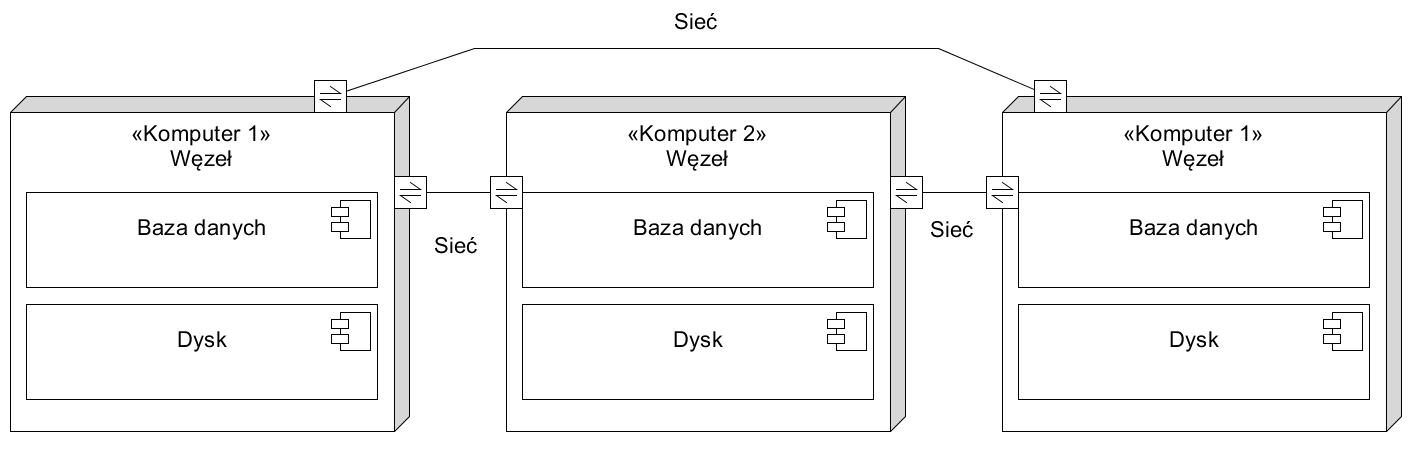
\includegraphics[width=15cm]{deployment_schema}
		\caption{Diagram struktury przykładowej instalacji z trzema węzłami}
		\label{fig:deployment_schema}
	\end{figure}

W rozważaniu zagadnienia, jakim są bazy danych, niezwykle ważnym aspektem jest skalowalność. Wymaganiem jest, aby baza była skalowalna zarówno poziomo jak i pionowo, liniowo w funkcji dostępnych zasobów sprzętowych. Spełnienie tego założenia wymaga konkretnych decyzji natury projektowej, które uwzględniono w strukturze bazy.

Istotnymi założeniami są również te natury infrastrukturalnej. Jako rozwiązanie programowe, do wdrożenia klastra niezbędne są konkretne zasoby sprzętowe, w stosunku do których istnieją również pewne wymagania. Przede wszystkim system (to jest interfejs oraz wszystkie węzły) musi działać w całości w zaufanej sieci lokalnej. Wszystkie hosty w tej sieci mają dostęp do odczytu i zapisu do innych węzłów i mogą łączyć się swobodnie ze sobą (muszą mieć realizacji logicznej topologii pełnej siatki). Musi być to sieć zaufana, gdyż węzły nie będą przeprowadzać uwierzytelniania, a napastnik z dostępem do sieci lokalnej byłby w stanie skutecznie sparaliżować pracę klastra. Elementy zapisujące dane w takiej bazie również musiałyby należeć do zaufanej sieci lokalnej. W przypadku geograficznego rozproszenia węzłów sieci można zastosować technologie wirtualizujące środowisko lokalne, takie jak VPN. Spełniają one bowiem warunek zaufanej sieci.

Ze względów organizacyjnych należy założyć także, że do danego ciągu zapisywać będzie tylko jeden element zespołu. Biorąc pod uwagę wdrożenie bazy jako systemu kontrolno-pomiarowego, jest to założenie logiczne i naturalne. Jeśli ciąg ewidencjonuje konkretny punkt pomiarowy w systemie, to jest to punkt unikatowy i z pewnością będzie istniał jeden element zapisujący ten ciąg. Jak wspomniano wcześniej, dysponuje on wiedzą na temat ciągu, który zapisuje. Wynika to z konstrukcji systemu, w której wiele modułów komunikacyjnych zainstalowanych na monitorowanych obiektach łączy się z niezależnie i równolegle pracującymi agentami po stronie serwera. Agenty te następnie zapisują zebrane dane do bazy danych. Schematycznie przedstawiono tą sytuację na rysunku \ref{fig:smok_generaldataflow}. Ponieważ pojedynczy agent odpowiada za wszystkie ciągi danego obiektu, założenie to jest spełnione.

	\begin{figure}[h]
		\centering 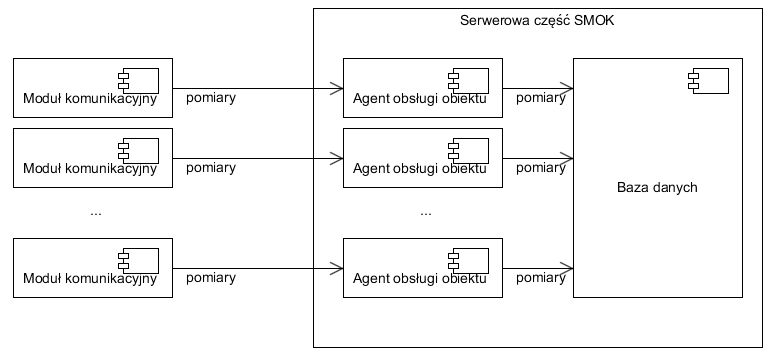
\includegraphics[width=15cm]{smok_generaldataflow}
		\caption{Diagram ogólnej idei przepływu danych}
		\label{fig:smok_generaldataflow}
	\end{figure}

Ze względu na uproszczenie projektu zdecydowano się, aby założyć, że dany ciąg w całości zmieści się na jednym węźle. Nie jest to wymóg w żaden sposób przesadzony – wstępne szacunki zakładają że do przechowania roku pomiarów wartości zmiennoprzecinkowej zdejmowanych co 5 sekund nie powinno być potrzebne (zaniedbując dodatkowe narzuty) więcej niż 72 MB\footnote{Założono 8 bajtów na znacznik czasu oraz 4 bajty na wartość.}.

Baza jako system modularny i mający wiele aspektów działania składa się z współpracujących ze sobą elementów. Każdy z nich zapewnia konkretną funkcjonalność, jednak dopiero razem stanowią zgodny z założeniami program. Ogólny diagram modułów i ich powiązań przedstawiono na rysunku \ref{fig:general_structure}. Projektowane rozwiązanie składa się z następujących modułów:

	\begin{figure}[h]
		\centering 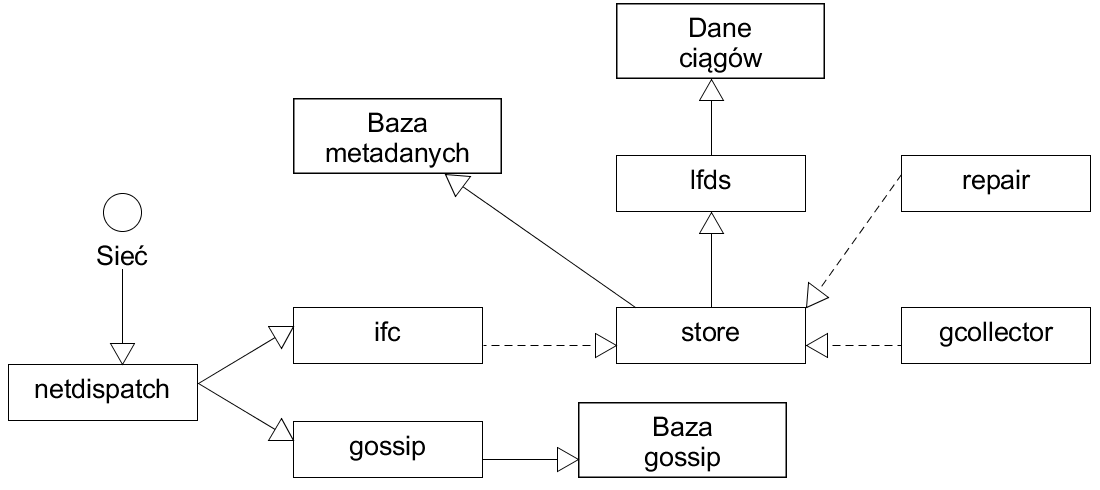
\includegraphics[width=15cm]{general_structure}
		\caption[Prezentacja modułów i ich wzajemnych powiązań]{Prezentacja modułów i ich wzajemnych powiązań. Pogrubione ramki oznaczają repozytoria danych, strzałki linią przerywaną oznaczają relatywnie ,,luźniejsze`` sprzężenie.}
		\label{fig:general_structure}
	\end{figure}

\begin{itemize}

\item \textit{netdispatch} odpowiada za przyjmowanie połączeń sieciowych za pomocą gniazdek TCP, a następnie przekazywanie ich do dwóch modułów które korzystają z łączności sieciowej,

\item \textit{gossip} ma za zadanie koordynację z innymi węzłami i utrzymuje w danym węźle reprezentację innych węzłów w klastrze --- ich adresów, stanów awarii i konfiguracji. \textit{Gossip} wymienia się tymi danymi z innymi węzłami w określony sposób, zapewniając aktualność danych. Ogólny opis jego działania podano w p. \ref{sec:keyproblems},

\item \textit{ifc} stanowi interfejs między binarnym protokołem sieciowym a modułami wykonawczymi systemu. Wykonuje on komendy zadane przez klienta przy użyciu modułu \textit{store} i odsyła wyniki. \textit{ifc} odpowiada również za przekierowanie rozkazu, jeśli okaże się że węzeł z jakichś przyczyn nie może wykonać otrzymanego rozkazu,

\item \textit{store} to moduł koordynujący dostęp do danych zgromadzonych na węźle. Zapewnia on funkcjonalności dotyczące tworzenia oraz kasowania ciągów. Zawiera także interfejsy do dodawania i odczytywania danych pomiarowych,

\item \textit{lfds} odpowiada za fizyczną, dyskową reprezentację zgromadzonych danych. Dba o to, aby w szybki sposób można było odnaleźć żądane wycinki danych oraz o zagadnienia synchronizacji dostępu,

\item \textit{gcollector} zapewnia wsparcie dla kasowania ciągów. Ze względu na założony model bazy danych jest on niezbędny aby kasowanie mogło być dokonane w sposób zsynchronizowany na wielu węzłach jednocześnie,

\item \textit{repair} dokonuje napraw danych ciągu, jeśli zostanie wykryty brak spójności danych. Działa on w tle, do minimum redukując zakłócenia związane z swoją pracą.
\end{itemize}

\subsection{Kluczowe problemy i ich rozwiązanie}
\label{sec:keyproblems}
Ponieważ zdecydowano się na zarządzanie rozproszeniem bazy poprzez uczynienie wszystkich węzłów równorzędnymi, pojawia się dodatkowy problem. Mianowicie brak jest centralnego katalogu, który przechowywałby informację o węzłach obecnych w systemie, ich stanie oraz informacji, które pozwolą ustalić, który węzeł odpowiedzialny jest za konkretny ciąg. Informacje takie są kluczowe, zwłaszcza w momencie, gdy system otrzymuje żądanie odczytu bądź zapisu. Musi on wtedy, w szybkim tempie, ustalić, do którego węzła trafi polecenie.

Zdecydowano się tutaj na podobne rozwiązanie jakie zostało zastosowane w bazie danych Cassandra \cite{Lakshman:2010:CDS:1773912.1773922} pod nazwą \textit{gossip}. Rozwiązanie to polega na wymienianiu się przez węzły fragmentarycznymi informacjami o stanie swoim i innych węzłów. Przy wystarczającej ilości takich wymian dany węzeł będzie znał stan wszystkich węzłów w danym klastrze. Wymienianie się takimi komunikatami zgodnie z pewnymi regułami zapewnia, że aktualizacje stanu będą propagowane zarówno szybko, jak i do wszystkich innych węzłów.

Każdy węzeł dysponować będzie informacjami o adresach i znanym stanie każdego innego węzła w klastrze. Taka struktura danych nie musi być większa niż ok. 200 bajtów na węzeł, co w przypadku nawet dużych klastrów nie będzie w znaczący sposób wywierać istotnego negatywnego wpływu na zużycie pamięci. Celem zainicjowania takiej tabeli przy rozruchu węzła podawać będzie się mu adres innego węzła, który będzie dysponował już jakimiś informacjami nt. klastra (tj. będzie już weń włączony). Taki węzeł startowy następnie roześle informację innym węzłom o nowym elemencie klastra.

Przy jakiejkolwiek modyfikacji stanu klastra, czy wykryciu że jeden z węzłów uległ awarii, taki system równorzędnej wymiany wiadomości o stanie klastra sprawi że w skończonym czasie wszystkie składowe będą miały spójny obraz o stanie całości systemu. Dzięki temu będą w stanie na jego podstawie podejmować decyzje. Warto jednak zadbać o to, aby nie zdarzyła się sytuacja, w której dwie aktualizacje stanu tego samego węzła będą ze sobą konkurować. Każda informacja o danym węźle musi być opatrzona znacznikiem czasowym, nadawanym przez wysyłającego. Wtedy, węzeł odbierając dwie nawet sprzeczne informacje, będzie w stanie zaktualizować swoją bazę tą nowszą, zapewne bardziej zbieżną z rzeczywistością, informacją.

Istotnym problemem, który rozwiązano jest metoda mapowania ciągów oraz ich kopii zapasowych na węzły. Rzecz tyczy się tego, jak po nazwie, czy też definicji ciągu, określić węzeł, na którym się znajduje. Jak wcześniej ustalono, klaster pracować będzie bez węzła typu master, tak więc nie istnieje centralny katalog ewidencjonujący wszystkie ciągi obecne w systemie. Zdecydowano się rozwiązać to za pomocą systemu mieszania opisanego w rozdziale \ref{sec:dht}.

\begin{listing}
\linespread{1} \small \lstinputlisting[label=lst:hashing, language=Java, captionpos=b, caption=Funkcja mieszajacą biorąca pod uwagę także numer repliki danej]{hashing_function.java} \linespread{\WorkLineSpread} \normalsize
\end{listing}

Oczywiście rozwiązanie to w podstawowym formacie nie będzie współgrać z założeniem redundancji danych. Aby określić dodatkowe węzły odpowiedzialne za dany ciąg, można dodać do wartości funkcji mieszającej pewną stałą wartość. Sprawi ona, że oznaczony zostanie węzeł znajdujący się na „przeciwnej” stronie pierścienia wartości – więc z pewnością inny niż ten, który uległ awarii. Taki sposób mieszania ilustruje funkcja wchodząca w skład bazy, przedstawiona na listingu \ref{lst:hashing}. Graficzna interpretacja takiego sposobu przedstawiona jest na rysunku \ref{fig:interp_token_ring_replicas}. Z przyczyn praktycznych ograniczono maksymalną ilość replik\footnote{kompletnej kopii wszystkich danych konkretnego ciągu} do czterech. Nie zakłada się, że będą definiowane więcej niż 4 repliki danego ciągu. Dodanie większej liczby wymaga po prostu uzupełnienia dodatkowych współczynników w funkcji mieszającej, więc takie ograniczenie nie będzie to stanowiło praktycznego problemu.

	\begin{figure}[h]
		\centering 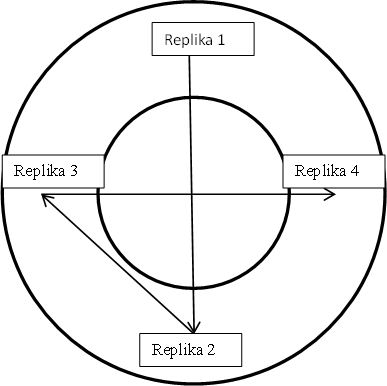
\includegraphics{interp_token_ring_replicas}
		\caption{Graficzna interpretacja przydziału węzłów odpowiedzialnych za repliki, w zbiorze wartości funkcji mieszającej}
		\label{fig:interp_token_ring_replicas}
	\end{figure}

Kolejne zagadnienie dotyczy definiowania ciągów. Aby utrzymać spójność systemu, każdy z węzłów musi dysponować identyczną definicją. Możliwa jest także sytuacja, w której węzeł odpowiedzialny za jedną z replik w chwili tworzenia ciągu, nie będzie dostępny i ominie go komenda stworzenia ciągu. Podobna sytuacja może się zdarzyć w przypadku zmiany definicji ciągu.

Problem rozwiązano w nietypowy sposób, poprzez obowiązek pamiętania przez klienta definicji ciągu. Choć baza zapewnia możliwość pobrania definicji po nazwie ciągu\footnote{określonej jako ciąg znaków}, jednak przy zapytaniach odczytu bądź zapisu klient musi podać kompletną definicję ciągu. Oczekuje się, że klient będzie trzymał później tą definicję w pamięci podręcznej. Dzięki temu, jeśli ciąg nie istnieje, będzie mógł być utworzony, a dane pobrane z innych węzłów dysponujących replikami. Dodatkowo każda definicja ma pole \textit{generacji}. Jest to pole liczbowe określające która ,,wersją`` definicji jest podana. Jeśli węzeł dysponuje starszą, zostanie zastąpiona nowszą --- podaną przez klienta lub inny węzeł. Algorytm takiego zamieniania przedstawiono na rysunku \ref{fig:definition_resolution}. Dzięki takiemu rozwiązaniu węzły obsługujące repliki danego ciągu są w stanie skutecznie ustalić bieżącą definicję ciągu. Przewiduje się, że nie będzie się ona często zmieniać, a nawet jeśli, to dzięki skutecznemu systemowi numerowania wersji (generacji) definicji klaster będzie w stanie utrzymać spójność. Każda nowa redefinicja będzie musiała mieć zwiększony numer generacji.

	\begin{figure}[h]
		\centering 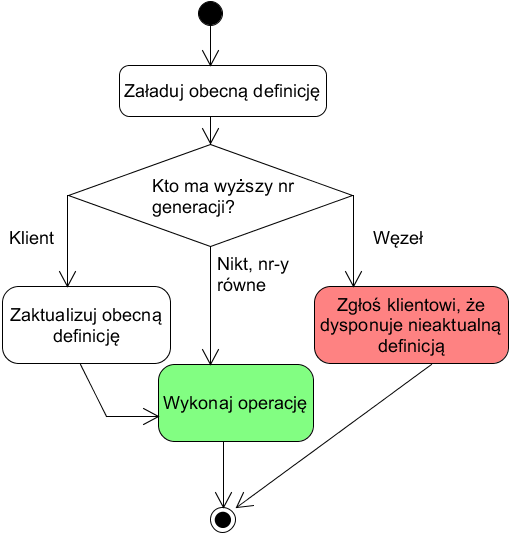
\includegraphics[width=8cm]{definition_resolution}
		\caption{Algorytm porównania i synchronizacji definicji}
		\label{fig:definition_resolution}
	\end{figure}

	\begin{figure}[h]
		\centering 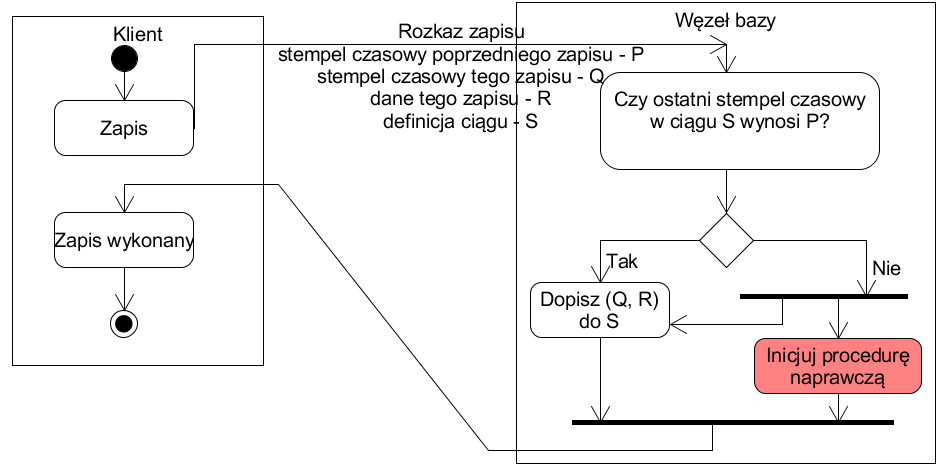
\includegraphics[width=14cm]{decgram}
		\caption{Algorytm detekcji niespójności ciągu}
		\label{fig:decgram}
	\end{figure}

Oczekuje się, że pamiętanie przez klienta w trakcie sesji kompletnej definicji ciągu nie będzie wielką przeszkodą. Zwykle to jeden klient dopisuje dane do jednego ciągu, więc ryzyko kolizji jest zredukowane do minimum, zwłaszcza jeśli projektant systemu przechowywania danych podejmie decyzję że tylko klient zapisujący jest uprawniony do redefinicji ciągu. Wymaganie to jest spełnione w przypadku systemu SMOK, gdzie takim klientem jest agent obsługi obiektu.

Innym problemem jest kasowanie ciągów. Ze względu na fakt, że jeden z węzłów obsługujących dany ciąg może być w trakcie awarii w czasie wydania takiego polecenia, komenda skasowania ciągu może go ominąć. Gdyby rozwiązanie to wykonać w sposób naiwny, to gdy taki węzeł zostanie naprawiony zreplikuje on innym węzłom ,,skasowany`` ciąg. Oznaczaoby to, że procedura usuwania ciągu będzie bezskuteczna. 

Rozwiązano to, dodając do definicji dodatkowe pole. Pole to informuje o tym, kiedy i czy dany ciąg został usunięty. Wzorowano się tutaj na rozwiązaniu o nazwie \textit{tombstone} zastosowanym w bazie Cassandra \cite{Lakshman:2010:CDS:1773912.1773922}. Tak więc kasowanie ciągu polega na zmianie jego definicji ustawiając wartość tego pola na obecny czas. Taki ciąg nie będzie replikowany innym węzłom, zaś jego dane (wartości pomiarów) zostaną skasowane, choć metadane pozostaną. Po upływie tzw. czasu bezpiecznego (np. tydzień) podsystem usuwania ,,starych`` metadanych taki wpis usunie. Rodzi to pewne problemy o których szerzej wspomniano w rozdziale \ref{sec:cluster_repair}.

Kolejnym problemem była detekcja spójności ciągu. W momencie kiedy pojedynczy ciąg śledzony jest jednocześnie na kilku węzłach --- w formie replik --- możliwym zjawiskiem jest to, że na pewien czas węzeł posiadający drugą, czy nawet trzecią replikę będzie zmuszony do odebrania tych zapisów jako jedyny. Pozostałe węzły, które w tym czasie były offline,  muszą dysponować metodą przywrócenia poprzednich danych gdy wykryją niespójność.

Zdecydowano się na rozwiązanie tego w nietypowej formie, niespotykanej w obecnych systemach bazodanowych. Mianowicie, każde żądanie zapisu, zawierające koniecznie rekord, zawiera również stempel czasowy poprzedniego zapisu. Klient, ze względu na strumieniowy charakter swojego zapisu, dysponuje taką informacją (zgodnie z zaleceniami z rozdziału \ref{sec:one_client_one_series}). W tym momencie, węzeł otrzymując żądanie zapisu, sprawdza czy rzeczywiście dysponuje rekordem o wartości stempla przesłanej jako poprzednia. Jeśli ten rekord istnieje, to można stwierdzić, że ciąg którym dysponuje węzeł jest spójny i kontynuować pracę. Jeśli nie zostanie on odnaleziony, należy zainicjować procedury naprawcze. Algorytm ten przedstawiono na rysunku \ref{fig:decgram}.

\subsection{Anatomia ciągu}
	\label{sec:anatomy}
	Ciąg, jako podstawowy element logiczny systemu, wymaga kilku słów opisu i wyjaśnienia. Jako element złożony, podzielić można go na dwie części --- dane oraz metadane. O formule danych wspomniano już w rozdziale \ref{sec:assumptions}, tak więc fakt przechowywania ich jako uporządkowanych po czasie par stempel czasowy-wartość jest oczywisty. Kłopotem może być dokładne oznaczenie pól metadanej ciągu. Zdecydowano się na następujące składowe takiego obiektu:
	\begin{itemize}
		\item \textit{seriesName} --- nazwa ciągu. Jest to podstawowy identyfikator danego ciągu w obrębie klastra. Dysponując nazwą można wystosować zapytanie o pobranie metadanych danego ciągu, tak więc stanowi ona taki ,,punkt wejścia`` do danego ciągu,
		\item \textit{replicaCount} --- ilość replik danego ciągu. Dysponując taką informacją można od razu ustalić ile węzłów będzie musiało zostać poinformowanych o zapisie nowego rekordu czy zmianie definicji ciągu,
		\item \textit{generation} --- numer generacji danego ciągu. Za każdym razem, kiedy jego definicja się zmienia, ta wartość jest zwiększana o jeden. Dzięki temu, gdy węzły odpowiedzialne za dany ciąg dysponują jego różnymi definicjami, będą w stanie ustalić, która z nich jest obowiązująca,
		\item \textit{autoTrim} --- opcja ta służy do automatycznego usuwania danych uznanych za ,,stare``. Jeśli wartość pola wynosi 0, to żadne dane nie będą usuwane. Jeśli natomiast jest pozytywna, to dane starsze niż \textit{autoTrim} (w sensie wartości stempla czasowego) od aktualnego najnowszego wpisu będą oznaczane jako dostępne do skasowania. Sterownik przechowywania danych nie jest zobligowany do ich natychmiastowego usunięcia, a system może zwracać takie ,,stare`` dane.
		\item \textit{recordSize} --- rozmiar pola danych rekordu, w bajtach. Ta wartość określa jak długa jest część ,,danych`` rekordu. Do zasadniczego rozmiaru rekordu należy dodać jeszcze 8 bajtów na stempel czasowy. Rekordy w ramach danego ciągu muszą mieć tą samą długość --- co jest typowe w przypadku systemów pomiarowych, gdzie pomiar zawsze zamyka się w konkretnej liczbie bajtów,
		\item \textit{options} --- opcje przekazywane sterownikowi obsługującemu przechowywanie danych na dysku (patrz rozdział \ref{sec:part:lfds}),
		\item \textit{tombstonedOn} --- informacja o tym czy (i kiedy) ciąg został skasowany. Jeśli wynosi 0, to ciąg nie został skasowany. W przeciwnym razie jest tutaj stempel czasowy, kiedy wydano polecenie skasowania ciągu. Jeśli wartość tego pola jest niezerowa, to węzeł nie dysponuje danymi danego ciągu, więc na żądanie pobrania danych czy dopisania rekordu zwróci informację o braku tegoż ciągu.
	\end{itemize}

	Jeśli ciąg nie jest skasowany, to istnieją także jego dane. Konkretny format zapisu tych danych zależy od danego sterownika LFD (patrz p. \ref{sec:part:lfds}), nie mniej jednak zawsze na on charakter uporządkowanego ciągu rekordów. Ciąg ten może być kompletny, lub nie (jeśli węzeł uległ wcześniej awarii). Zdekompletowany ciąg do którego dopisuje się dane będzie dysponował też jednym lub więcej ciągami pomocniczymi, przechowującymi tymczasowo zapisy, dopóki ,,główny`` ciąg nie zostanie uzupełniony brakującymi danymi z innych węzłów, pobranymi w procesie naprawczym. Dokładny opis procesu naprawczego podano w rozdziale \ref{sec:part:store}.

\docsection{Opis modułów programu bazodanowego}

		Wykonana baza danych, jako program o średnim rozmiarze\footnote{2845 linijek kodu} wymagał modularyzacji. Jest to podejście standardowe w przypadku projektów informatycznych i zapewnia ważne zalety, takie jak uproszczenie wymiany informacji między podzespołami czy uproszczona konserwacja i opis działania programu. Zastosowano zarówno moduły zewnętrzne, jak i moduły stworzone na potrzeby bazy. W rozdziale podano szczegółowy, techniczny opis modułów bazy oraz specyfikację protokołu sieciowego którym posługuje się baza.

%	\subsection{Google GSON}
%		Programy działające w tle bez interakcji ze strony użytkownika --- w realiach uniksowych nazywane \textit{demonami}, podobnie jak większość złożonych programów wymagają konfiguracji (lub przynajmniej muszą mieć taką możliwość). Standardem przemysłowym w tym względzie są tzw. pliki konfiguracyjne, zapisywane w różnym formacie. Zdecydowano się na użycie formatu JSON\cite{json}, ze względu na łatwość edycji i logiczne uporządkowanie.

 %		Oczywistym jest, że taki plik należy wczytać do postaci użytecznej przez kod języka Java. Do tego celu zastosowano bibliotekę GSON\cite{gson}, pierwotnie opracowaną na wewnętrzne potrzeby firmy Google. Biblioteka ta jest w stanie, mając klasę języka Java, załadować do niej dane z pliku JSON, dzięki czemu minimalizuje potrzebę pisania dodatkowego kodu. 

	\subsection{startup --- uruchomienie bazy i konfiguracja}
		Zadaniem modułu \textit{startup} jest wczytanie plików konfiguracyjnych, oraz uruchomienie wątków składowych węzła. Zakłada się, że plik konfiguracyjny znajduje się w katalogu uruchomieniowym programu i nazwa się \textit{config.json} --- założenie to można zrewidować zmieniając ścieżkę w kodzie programu. Uruchamia on wątki składowe - takie jak wątek naprawczy, wątek \textit{gossip} oraz wątek połączeń TCP, a także, jeśli zostanie to uznane za konieczne, inicjuje pobranie informacji o klastrze z wskazanego węzła.

     \subsection{gcollector --- odśmiecacz metadanych}
             \label{sec:part:gcollector}
Jak wspomniano w rozdziale \ref{sec:assumptions}, metadane skasowanego ciągu, w przeciwieństwie do jego danych, nie są kasowane od razu po otrzymaniu takiego rozkazu, a trzymane przez tzw. czas bezpieczny. Zadaniem \textit{gcollectora} jest periodyczne skanowanie bazy metadanych ciągów zdefiniowanych w danym węźle oraz fizyczne usuwanie ich, jeśli są one oznaczone jako skasowane oraz wystarczająco stare.

Dokonywane jest to poprzez uruchomienie przy starcie bazy osobnego wątka odśmiecacza. Co czas bezpieczny skanuje on całą bazę metadanych. Żeby dane te zostały fizycznie skasowane, muszą być spełnione dwa warunki --- ciąg musi być oznaczony jako skasowany (znacznik \textit{tombstone}) oraz od czasu oznaczenia musi minąć przynajmniej czas bezpieczny. Jeśli te warunki są spełnione, za pomocą menedżera danych definicja ciągu jest fizycznie usuwana.

Ideą ciągu bezpiecznego jest to, że awaria węzła nigdy nie będzie trwała dłużej niż ten czas (jeśli tak, to należy usunąć wszystkie dane z węzła przed włączeniem go ponownie), tak więc będzie to czas przez który ,,skasowane`` metadane będą istniały w systemie. Po tym czasie, niezależnie od stanu awarii węzłów, za które były te ciągi odpowiedzialne, metadane nie będą już obecne w klastrze.

     \subsection{gossip --- komunikacja stanu węzłów}
		Projektowana baza danych, jak system nie dysponujący węzłem typu master, musi dysponować konkretnym mechanizmem utrzymywania informacji o stanie klastra, jego składowych oraz ich parametrach. Do tego celu służy mechanizm \textit{gossip}. Prowadzi on także wewnętrzną bazę danych stanu i parametrów innych węzłów.

	Baza danych węzłów jest elementem niezbędnym do funkcjonowania reszty systemu. Pozwala ona przede wszystkim na podstawie nazwy ciągu i numeru repliki określić węzeł zań odpowiedzialny, a także stwierdzić, że węzeł ten uległ awarii. Po otrzymaniu od innego węzła --- spodziewanej lub nie --- informacji o stanie klastra (bądź jego wycinka), gossip sprawdza czy dane te są nowsze (każda informacja bowiem opatrzona jest stemplem czasowym) i jeśli są, wprowadza je do stanu wiedzy węzła. \textit{Gossip} służy także detekcji błędów. Gdy z jakiegoś powodu komunikacja z innym węzłem zawiedzie, zwiększany jest licznik awarii komunikacji z danym węzłem. Jeśli komunikacja powiedzie się, licznik ten jest resetowany. Dopiero gdy przekroczy on pewną wartość, docelowy węzeł oznaczony jest jako niesprawny, a informacja ta przesyłana jest innym węzłom. Nie można wyciągnąć wniosku o awarii konkretnego węzła, jeśli błąd wystąpi tylko raz, albowiem może to wynikać z szeregu innych przyczyn (chwilowe przeciążenie, przejściowa awaria sieci), więc każdy błąd musi być potwierdzony kilkukrotną obserwacją.

	Oczywiście gdy węzeł ma do przekazania innym dane, nie rozsyła ich do wszystki węzłów. Takie podejście podnosiłoby złożoność komunikacyjną systemu do $O(n^2)$, wymagając pełnej siatki topologicznej. W przypadku większych klastrów, sieć dosłownie zalewana byłaby komunikacją. W takiej sytuacji wymagane jest inteligentne rozwiązanie.

	Rozwiązanie to zapobiega wysyceniu sieci w sposób dwufazowy. Jeśli węzeł odbierze informacje co do których stwierdzi że są nowe, dopisze je do swojej kolejki nowych informacji. Komunikacja nie jest więc bezpośrednio inicjowana poprzez odebranie nowych danych. Co 4 sekundy wątek \textit{gossip} sprawdza czy są nowe informacje które powinny być rozesłane. Jeśli tak jest, wylosuje z swojej listy węzłów 5 pozycji do których spróbuje przesłać te nowe dane. Dodatkowo, jeśli nie wylosował swojego bezpośredniego sąsiada po prawej stronie, doda go do tej listy, końcowo będzie to 5 lub 6 pozycji. Mechanizm ten ilustruje rysunek \ref{fig:gossip_mirv}. To obostrzenie zapewnia że w końcu wszystkie węzły otrzymają zaktualizowaną informację, choćby miało się to stać w czasie $O(n)$. Ze względu na losowanie i późniejsze rozsyłanie wiadomości do 5 węzłów przez każdy następny, stanie się to zazwyczaj dużo szybciej.

	\begin{figure}[h]
		\centering 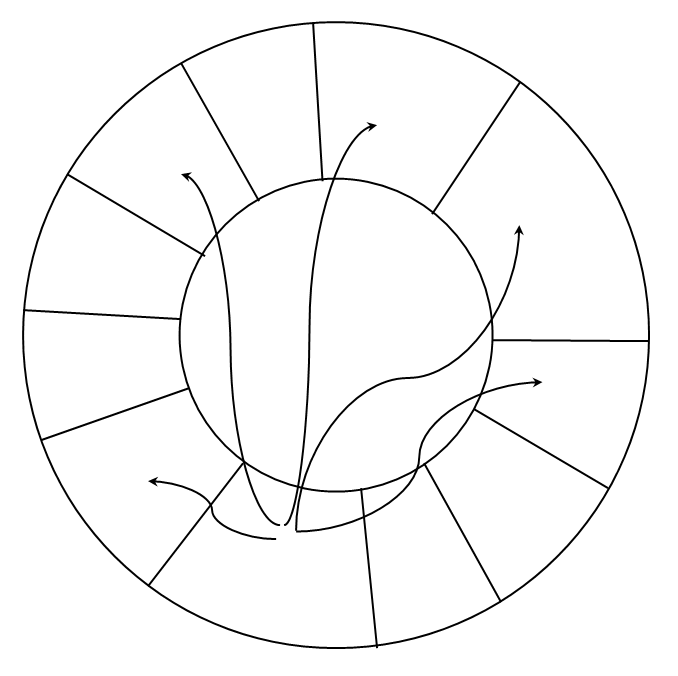
\includegraphics[width=8cm]{gossip_mirv}
		\caption[Ilustracja rozsyłania danych o węzłach za pomocą \textit{gossip}]{Ilustracja rozsyłania danych o węzłach za pomocą \textit{gossip}. Węzeł źródłowy wysyła komunikat do 5 wylosowanych węzłów, w których zawiera się również jego bezpośredni prawy sąsiad. To, czy każdy z docelowych węzłów podobnie retransmituje informacje zależy od tego czy wykorzysta ją do aktualizacji stanu swojej wiedzy.}
		\label{fig:gossip_mirv}
	\end{figure}

	Jeśli zaś \textit{gossip} nie ma żadnej nowej informacji do przetransmitowania, wybierze on 2 węzły (również w razie potrzeby dodatkowo doliczając prawego sąsiada) co do których sprawdzi czy jest w stanie się z nimi skomunikować. Jeśli próba zawiedzie, zostanie zwiększony lokalny licznik awarii tych węzłów --- przy odpowiedniej liczbie powtórzeń awarii reszcie klastra zostanie przesłana informacja o awarii węzła, z którym komunikacja wielokrotnie zawiodła.

	Ciekawym problemem jest budowanie bazy na początku rozruchu klastra. Otóż mając szereg węzłów bez informacji startowej o sobie nawzajem niemożliwe jest zbudowanie takiej bazy. Wymagane jest więc, aby węzeł który zostaje uruchomiony miał jakąś możliwość nawiązać kontakt przynajmniej z jednym węzłem. Ten problem rozwiązuje instytucja tzw. węzła startowego. Podczas rozruchu na podstawie pliku konfiguracyjnego węzeł podejmuje decyzję, czy wystosować do zdalnego węzła opisanego w swoim pliku prośbę o przesłanie całej swojej mapy danych oraz informację o sobie, tak aby węzeł startowy mógł poinformować resztę klastra. Oczywiście węzeł startowy przy rozruchu może nie nawiązywać połączenia z żadnym innym węzłem, wszak to inne węzły skomunikują się z nim. Możliwa jest także konfiguracja gdzie dwa węzły startowe komunikują się przy starcie ze sobą, a jedna część klastra rozpoczyna inicjalizację od jednego z nich, a druga od drugiego. Węzeł startowy w żaden sposób nie jest uprzywilejowany, a służy jedynie do wstępnej propagacji danych o klastrze.

W takiej sytuacji może być jednak ciekawe zjawisko. Przypuśćmy że klaster z jednym węzłem startowym uruchomił się pomyślnie. Następnie dochodzi do awarii węzła startowego, po czym zostaje on zrestartowany. Problem jest teraz tylko tego typu, że węzeł startowy nie dysponuje żadną informacją na temat innych węzłów! Rozwiązanie tego problemu wymaga jednego dodatkowego założenia przy komunikacji \textit{gossipa}. Zasadę tą można sformułować następująco: ,,jeśli skomunikuje się z tobą węzeł o adresie którego nie masz w swojej bazie węzłów, to zażądaj od niego wysłania swojej bazy wszystkich węzłów``. Ponieważ system utrzymuje zachowanie sprawdzania komunikacji z innymi węzłami --- nawet tymi, co do których stwierdzono awarię --- prędzej czy później powrót węzła zostanie wykryty, a jego stan wiedzy szybko zaktualizowany.

	\subsection{netdispatch --- multiplekser połączeń TCP}
Celem uproszczenia konfiguracji sieciowej systemu zdecydowano się na ograniczenie liczby serwerowych gniazdek TCP wykorzystywanych przez serwer. Z tego powodu do wszelkiej komunikacji sieciowej wykorzystywane jest tylko jedno gniazdo TCP. Rodzajów komunikacji natomiast jest kilka, wyróżnić można chociaż transfer danych ciągów czy komunikację typu gossip. Z tego też powodu moduł netdispatch służy do multipleksowania odbieranych połączeń do różnych modułów. Typ połączenia określany jest przez pierwszy odebrany przezeń bajt, następnie połączenie przekazywane jest do odpowiedniego, innego modułu.

     \subsection{lfds --- przechowywanie danych ciągu}
		\label{sec:part:lfds}
Jednym z kluczowych aspektów projektowanej bazy danych jest możliwość przechowywania ich na dysku. Taką możliwość zapewnia właśnie podsystem \textit{LFD} (\textit{Local Filesystem Driver}). Przede wszystkim należy zacząć od opisania jaką funkcjonalność powinien zapewniać taki podsystem. Celem modularyzacji systemu oraz możliwości stosowania różnych sposobów zapisu, nawet w obrębie jednego klastra. Zdecydowano się na definicję \textit{LFD} jako interfejsów języka Java oraz stworzenie jednej, prostej ale skutecznej, implementacji tego zestawu interfejsów.

Zastosowanie tutaj interfejsów zamiast konkretnej implementacji pozwala dostosowywać w szerszy sposób bazę danych do swoich potrzeb. Jeśli potrzebny byłby inny schemat fizycznego zapisu niż napisany jako referencyjny, można zawsze stworzyć własną implementację interfejsów \textit{LFD}, korzystającą chociażby z relacyjnej bazy danych, lub nawet z innego systemu przechowywania danych pomiarowych.

Przede wszystkim podstawową jednostką w tym przypadku będzie ciąg \textit{LFD}, opisywany przez nazwę, rozmiar pola danych rekordu oraz dodatkowe opcje, których implementacja zależna będzie od implementacji sterownika \textit{LFD}. Od ciągu przede wszystkim oczekuje się możliwości odczytu i dopisywania danych --- na razie nie martwiąc się o replikację czy metadane. Ze względu na prostotę nie przewiduje się tutaj możliwości modyfikowania istniejących danych. Dopuszcza się jedynie dopisywanie nowych rekordów, o stemplu czasowym większym od aktualnego maksimum (tzw. głowy ciągu). Musi też istnieć opcja kasowania takich ciągów. Mając więc pewne założenia co do obiektów na których wykonywane są operacje, dalej nazywanych ciągami \textit{LFD}, można przystąpić do zbudowania implementacji takowych.
	
Referencyjna implementacja, której nadano nazwę \textit{SUZIE}, do przechowywania danych ciągu \textit{LFD} wykorzystuje płaskie pliki, zawierające zapisane w uporządkowany sposób (rosnąco po stemplu czasowym) rekordy. Aby zmniejszyć czas dostępu do danych sterownik ten pozwala na dzielenie danych na pliki, rozmiar których można kontrolować za pomocą wspomnianych wcześniej opcji. Pliki te znajdują się w jednym katalogu, noszącym nazwę ciągu, tak więc sterownik ten wprowadza dodatkowe obostrzenie na nazwę ciągu, mianowicie by była ona poprawną nazwą katalogu w systemie plików na którym instalowana jest baza.

Pliki w których znajdują się dane ciągu nazywane są od stempla czasowego pierwszego rekordu, który się w nich zawiera. W ten sposób dysponując listą wszystkich plików można ustalić w którym pliku znajdzie się dany rekord. Dodatkowo, pliki których zapisywanie zostało definitywnie zakończone, co poznać można po utworzeniu pliku o nazwie ,,większej`` (w sensie numeracji) będą już otwierane tylko i wyłącznie w trybie do odczytu. Można to wykorzystać do zaaplikowania im optymalizacji na poziomie systemu plików (np. kompresja w NTFS). Wyjątkiem tutaj jest pierwszy plik danych --- tworzony w momencie inicjalizacji ciągu --- którego nazwa ustawiana jest na \texttt{0}.

Referencyjny sterownik LFD, obsługując dzielenie danych ciągu na wiele plików, musi dysponować mechanizmem który zdecyduje w której chwili plik do którego aktualnie prowadzony był zapis powinien być zamknięty, zaś do zapisu nowych rekordów stworzony nowy. Zachowanie sterownika \textit{SUZIE} można kontrolować, podając mu odpowiednie opcje. Możliwe jest to przy definicji (bądź późniejszej zmianie definicji) ciągu, w polu \textit{options} (opisane w rozdziale \ref{sec:anatomy}), podać można liczbę rekordów, po zapisaniu których zostanie stworzony nowy plik. Jeśli wartość ta nie zostanie podana, \textit{SUZIE} obliczy taką wartość żeby wynikowe pliki były nie większe niż 16 MB.

Wyszukiwanie danych w ciągu \textit{SUZIE} odbywa się dwufazowo. Pierwszym krokiem jest ustalenie listy plików które będą zawierać interesujące nas dane. Ponieważ zapytanie zawsze formułowane jest przy użyciu dwóch parametrów --- \texttt{od} oraz \texttt{do}, będzie to z pewnością ciągły zakres. Lista plików składowych ciągu jest sortowana rosnąco, a odpowiedni zakres wyszukiwany, co ilustruje listing \ref{lst:suzie_get_files}

\begin{listing}
\linespread{1} \small \lstinputlisting[label=lst:suzie_get_files, language=Java, captionpos=b, caption=Kod odpowiedzialny za ustalenie nazw plików zawierających podzbiór danych dotyczących zapytania.]{suzie_get_files.java} \linespread{\WorkLineSpread} \normalsize
\end{listing}

Następnie, na podstawie stworzonej listy plików, zwracany jest obiekt wyniku. Ponieważ gwarantowane jest, że dopóki przynajmniej jeden obiekt wyniku jest w użyciu (o co dba mechanizm zliczania referencji obiektu ciągu SUZIE) pliki nie będą kasowane, nie ma potrzeby późniejszego sprawdzania ich istnienia.

W obrębie plików ustalenie zakresu z którego będą pobierane dane sprowadza się do czterech możliwości:
\begin{itemize}
	\item \texttt{od} i \texttt{do} wypadają poza zakresami pliku, przeczytany liniowo zostanie cały plik,
	\item \texttt{od} i \texttt{do} wypadają wewnątrz pliku, zostanie przeczytany tylko jeden plik, w całości lub w swoim podzakresie,
	\item \texttt{od} wypada w pliku, \texttt{do} poza nim --- ten plik zostanie przeczytany jako pierwszy, od pewnego miejsca do końca,
	\item \texttt{od} wypada poza plikiem, \texttt{do} wypada w pliku --- ten plik zostanie przeczytany jako ostatni, od początku do pewnego miejsca wewnątrz tego pliku.
\end{itemize}

	Odnalezienie rekordu, dzięki faktowi, że są one uporządkowane po rosnących stemplach czasowych, jest zaskakująco szybkie. Wykorzystuje się tutaj mechanizm przeszukiwania binarnego, którego implementację umieszczono na listingu \ref{lst:binary_search}.

\begin{listing}
\linespread{1} \small \lstinputlisting[label=lst:binary_search, language=Java, captionpos=b, caption=Wycinek funkcji przeszukiwania binarnego.]{suzie_binary_search.java} \linespread{\WorkLineSpread} \normalsize
\end{listing}

Ze względu na elementarnie prosty format plików odczyty danych mogą przebiegać w sposób liniowy, najczęściej wiele rekordów na jedno systemowe wywołanie odczytu, do buforów w pamięci, bez analizy i dodatkowego przetwarzania każdego rekordu, co zapewnia dużą szybkość sterownika \textit{SUZIE}.

Pewnego zmartwienia nastręczać może synchronizacja czytelnik-pisarz. Problem ten rozwiązano w maksymalny sposób upraszczając format plików. Upewniając się że jedyną dozwoloną formą modyfikacji plików jest dopisywanie nowych rekordów, efektywnie zlikwidowano wpływ modyfikacji pliku na odczyt z niego w danej chwili.

Dodatkowym wyzwaniem które sterownik \textit{LFD} musi obsługiwać, jest funkcja \textit{autoTrim}, opisana w rozdziale \ref{sec:anatomy}. Ze względu na zakaz modyfikacji plików w inny sposób jak tylko dopisywanie danych, jednostką kasowania danych staje się tutaj cały plik. Dopiero, gdy warunek że wszystkie obiekty wyników są zamknięte można przystąpić do kasowania plików. Wtedy też uruchamiana jest procedura \textit{autoTrim}, jeśli jest wymagana. Dopiero gdy \textit{SUZIE} wykryje że plik zawiera tylko dane, które w całości mieszczą się za poza obrębem danych które mają być dostępne, jest on kasowany. W zależności od wybranego poprzez opcje rozmiaru plików może to powodować że nawet duża ilość danych archiwalnych będzie dostępna do odczytu, nawet mimo bardzo restrykcyjnego ustawienia \textit{autoTrim} na dany ciąg. Uruchamiając tą operację dopiero gdy wszystkie obiekty wyniku są zamknięte i blokowanie zwracania następnych obiektów tego typu do czasu ukończenia operacji zapewnia się spójność danych i eliminuje hazardy.

	\subsection{store --- menedżer danych i metadanych ciągów}
		\label{sec:part:store}
\textit{Store} jest mechanizmem łączącym przechowywanie danych ciągu oraz jego metadanych. Pośredniczy żądaniom odczytu i zapisu danych, oraz odpowiada za odpowiednią ich synchronizację, wraz z tworzeniem i modyfikowaniem ciągów. Sam \textit{store} składa się z trzech zasadniczych części --- \textit{SeriesDB}, \textit{SeriesController} i \textit{WriteAheadContext}.
	
\textit{SeriesDB} jest w ramach węzła singletonem. Stanowi podstawowy punkt wejścia do procesów operujących na ciągach oraz ich metadanych, zapewniając w ramach swoich działań synchronizację. Zajmuje się  redefinicją metadanych ciągów oraz tworzeniem obiektów \textit{SeriesController}.

\textit{SeriesController} jest klasą reprezentującą konkretny ciąg, zarówno w kontekście jego sterownika LFD i danych, jak i metadanych. Wywołania \textit{store} zapewniają, że dla danego ciągu w danej chwili będzie istniał maksymalnie jeden \textit{SeriesController}, dzięki temu obiekt ten może wewnętrznie przeprowadzać synchronizację bez konieczności koordynowania jej z innymi obiektami, co pozwala w istotny sposób uprościć implementację tego zagadnienia.

\textit{WriteAheadContext} jest klasą odpowiedzialną za pewne składowe procesu naprawczego. Ponieważ, jak wspomniano wcześniej, do ciągu LFD możliwe jest tylko dopisywane, a bazie nie wolno odmówić zapisu ze względu na zdekompletowany ciąg, wymagane jest miejsce na tymczasowe przechowywanie takich ,,zawieszonych`` rozkazów --- tych, które zostały przez bazę przyjęte, ale jeszcze nie dopisane do odpowiedniego zasadniczego ciągu LFD. Obsługę tej funkcjonalności zawiera właśnie \textit{WriteAheadContext}, tworzony dla konkretnego ciągu.

Jak już wcześniej wspomniano, \textit{SeriesDB} ma dwa zadania. Pierwszym z nich jest tworzenie i zarządzanie obiektami \textit{SeriesController}. Ponieważ z założenia musi istnieć tylko jeden taki obiekt na otwarty ciąg, \textit{SeriesDB} prowadzi także pamięć podręczną takich obiektów i zarządza nimi za pomocą zliczania referencji, dzięki czemu pozostałe elementy systemu korzystające z ciągów, zwłaszcza interfejs klienta, mogą operować w przejrzysty sposób. Drugim zasadniczym zadaniem \textit{SeriesDB} jest (re)definicja ciągów. Ponieważ z obiektem \textit{SeriesController} związana jest konkretna definicja ciągu, nie może ona zostać zmieniona w momencie gdy taki obiekt jest otwarty. Utrzymywana jest kolejka zadań redefinicji. Uruchamiane są one dla danego ciągu w momencie kiedy zostanie wykryte że jego obiekt \textit{SeriesController} nie znajduje się w użyciu. Dodatkowo nowy \textit{SeriesController} nie zostanie utworzony gdy redefincja nie została ukończona. Dzięki tej operacji zachowuje się gwarancję synchronizacji.

Oczywiście usuwanie ciągu z pamięci w momencie kiedy nie jest on już używany może wydawać się dobrym pomysłem, jednak jest to zachowanie szkodliwe z punktu widzenia długoterminowej wydajności. \textit{SeriesDB} implementuje więc pamięć podręczną. Rozmiar jej można ustawić w pliku konfiguracyjnym. Stwierdzono że logika LRU\footnote{Least Recently Used}, polegająca na zliczaniu częstotliwości użycia danego ciągu i w przypadku przekroczenia rozmiaru pamięci podręcznej eksmisja z niej najrzadziej wykorzystywanych ciągów, nie będzie pomocna w przypadku użycia gdy wszystkie (lub większość) ciągów są periodycznie wykorzystywane w celu dopisania wartości. Z tego powodu też zdecydowano się na odmienne, prostsze podejście. W momencie przekroczenia rozmiaru pamięci podręcznej usuwane są z niej wszystkie ciągi, które aktualnie nie znajdują się w użyciu. Testy prowadzone w trakcie tworzenia bazy dowiodły że zysk polegający na implementacji pamięci podręcznej w ten sposób w porównaniu do usuwania ciągów z pamięci w momencie ich zamknięcia uzasadnia jej użycie.

Przechowywanie metadanych przez \textit{SeriesDB} zrealizowane jest w prosty sposób. W katalogu, określonym w pliku konfiguracyjnym, znajdują się pliki o nazwach odpowiadających nazwom ciągu. Pliki te zawierają zserializowane (za pomocą mechanizmów serializacji języka Java) definicje metadanych. Zdecydowano się na serializację Java, gdyż nie ma wymogu co do czytelności, czy też możliwości edycji "przez człowieka" tych danych, a serializacja jest jednym z szybszych sposobów wczytywania tych obiektów. Prędkość istotnie jest zagadnieniem istotnym, gdyż metadane wczytywane są za każdym razem kiedy otwierany jest ciąg który nie znajduje się w pamięci podręcznej \textit{SeriesDB}.

Obiekt \textit{SeriesController} reprezentuje konkretny ciąg, posiadający ustaloną definicję. Definicja ta pozostaje niezmienna w czasie życia obiektu. Stanowi on podstawową bramę do przeprowadzania operacji na ciągu, jakich jak odczyt danych, dopisanie rekordu czy chociażby pobranie ostatnio dopisanego stempla czasowego. Zawiera on również implementację operacji skasowania danych ciągu (nie metadanych, gdyż jest to zadaniem \textit{SeriesDB}). Najistotniejszym jednak działaniem \textit{SeriesController} jest branie udziału w wykrywaniu zdekompletowania ciągu i współpraca z \textit{WriteAheadContext} oraz modułem naprawczym w celu ,,uzdrowienia`` ciągu. Każde polecenie zapisu oprócz kompletnego rekordu zawiera również stempel czasowy ostatnio zapisanego. W momencie gdy wartość ta nie zgadza się z rekordem zapisanym w bazie, uruchamiany jest proces naprawczy. Zapis przejmuje \textit{WriteAheadContext}, oraz informowany o awarii jest wątek naprawczy. W momencie gdy uzupełnione zostaną brakujące dane, jest o tym informowany \textit{WriteAheadContext} który scala zebrane dane w spójną całość. \textit{SeriesController} odpowiedzialny jest również za realizację opcji \textit{autoTrim}, wysyłając sterownikowi \textit{LFD} rozkazy co do ,,ucinania`` zbioru danych. Operację zapisu widzianą z poziomu \textit{SeriesController} przedstawiono na listingu \ref{lst:seriescontroller_write}.

\begin{listing}
\linespread{1} \small \lstinputlisting[label=lst:seriescontroller_write, language=Java, captionpos=b, caption=Operacja dopisania rekordu w \textit{SeriesController}.]{seriescontroller_write.java} \linespread{\WorkLineSpread} \normalsize
\end{listing}

Istotną częścią organizacji danych podczas naprawy zajmuje się podległa \textit{SeriesController} instancja klasy \textit{WriteAheadContext}. Jak już wcześniej wspomniano, ze względu na fakt że wykorzystywany interfejs \textit{LFD} pozwala jedynie na dopisywanie nowych rekordów i odczyt zakresów, wymagana jest tymczasowa pamięć na przechowanie zapisów podczas naprawy ciągu. Nie można bowiem dopisać do zasadniczego ciągu \textit{LFD} nowych wartości, gdy ,,w środku`` znajdowałaby się luka. Zadanie przetrzymania tych nowo dodawanych danych podczas gdy ciąg nie jest jeszcze naprawiony zajmuje się właśnie \textit{WriteAheadContext}.

Do zasadniczego ciągu przypisanych może być dodatkowo kilka ciągów dodatkowych, służących do przechowywania takich danych. W najprostszym przypadku pojawi się jeden taki ciąg. Rozważmy przypadek gdy węzeł, ze względu na awarię, przeoczył pewien ciąg zapisów. W momencie gdy pojawi się rozkaz zapisu z ,,poprzednim stemplem czasowym``, tworzony jest ciąg pomocniczy o nazwie równej wartości ,,poprzedniego stempla czasowego``. Będzie on miejscem gdzie wędrować będą nowe zapisy. Równocześnie zostanie uruchomiony proces naprawczy, który po pewnym czasie uzyskawszy brakujące dane zapisze je do głównego ciągu. Gdy dojdzie już do elementu który stanowił ,,poprzedni stempel czasowy``, ciąg pomocniczy zostanie w całości dopisany do ciągu głównego. Następnie ciąg pomocniczy zostanie usunięty, zaś nowe zapisy będą od razu dodawane do ciągu głównego.

Oczywiście może wydarzyć się sytuacja w której węzeł ponownie ulegnie awarii, nawet nie zdążywszy naprawić ciągu. W takim razie pojawi się kolejna luka w systemie. Kolejne zapisy do ciągu umieszczone będą już nie w pierwszym ciągu pomocnicznym, gdyż logicznie po tym ciągu były jakieś zapisy. Stworzony zostanie nowy ciąg pomocniczy, noszący nazwę kolejnego ,,poprzedniego stempla czasowego``. Taką hipotetyczną sytuację ilustruje rysunek \ref{fig:repair_lossage_1}. 

Istotnym zastrzeżeniem jest również to, że operacja zapisu przedstawiana przez \textit{SeriesController} służy zarówno do dopisywania danych otrzymanych od użytkownika, jak i do przeprowadzana procesu naprawczego. W przypadku takiej sytuacji \textit{WriteAheadContext} musi poprawnie zdecydować do którego ciągu konkretny element powinien być dopisany, oraz --- w razie czego --- połączyć ciągi w jeden.

	\begin{figure}[h]
		\centering 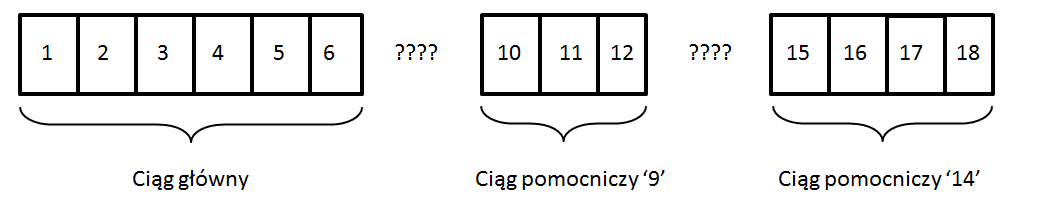
\includegraphics[width=16cm]{repair_lossage_1}
		\caption[Graficzna reprezentacja możliwego stanu ciągu po dwóch awariach]{Graficzna reprezentacja możliwego stanu ciągu po dwóch awariach. Pierwsza awaria nastąpiła po zapisie rekordu 6. Kolejny zapis (o poprzednim stemplu 9) poskutkował stworzeniem ciągu pomocnicznego `9`. Kolejna awaria wystąpiła zanim ciąg mógł zostać naprawiony i węzeł otrzymał dopiero rozkaz zapisu rekordu `15` z poprzednim stemplem równym `14`. Utworzony został więc pomocniczy ciąg `14`. Ciągi te będą reintegrowane z głównym ciągiem gdy moduł naprawczy wyda polecenie zapisu rekordu o stemplu równym nazwie ciągu pomocniczego.}
		\label{fig:repair_lossage_1}
	\end{figure}

\textit{WriteAheadContext} odpowiedzialny jest również za dopisanie ciągów pomocnicznych do ciągu głównego gdy dostępne są już brakujące dane. Ciągi pomocnicze również korzystają z interfejsów \textit{LFD}, co upraszcza konstrukcję systemu. Może to hipotetycznie posłużyć do korzystania z dwóch różnych sterowników \textit{LFD} --- jednego do przetrzymywania ciągów pomocniczych, a drugiego do głównego (z definicji niemalże dłuższego i ważniejszego) ciągu danych.

	\subsection{repair --- naprawa uszkodzonych ciągów}
Mimo obecności podsytemu danych służących do radzenia sobie z sytuacjami awaryjnymi, musi istnieć pewien moduł który będzie reagował na zgłoszone uszkodzenia ciągów i dokonywał napraw. Taką funkcjonalność implementuje moduł \textit{repair}.
	
Podstawowym punktem wejścia w module jest wątek nadzorcy naprawy. Wątek ten otrzymuje informacje od \textit{SeriesController} o konieczności inicjacji naprawy danego ciągu. Jeśli przez czas ok. 24 sekund nie otrzyma żadnych informacji, dokona on próby przeskanowania katalogu z ciągami pomocniczymi. Mogła bowiem nastąpić sytuacja w której wykryta została awaria ciągu, ale węzeł ponownie został wyłączony. W tym wypadku pozostanie ślad w postaci utworzonego ciągu pomocnicznego, ale \textit{SeriesController} wykryje awarie dopiero po otrzymaniu kolejnego żądania zapisu.

W momencie identyfikacji potrzeby naprawy ciągu, wątek-nadzorca sprawdzi czy nie jest to duplikat poprzednio złożonego zgłoszenia i w razie potrzeby wyeliminuje go. Zostanie również sprawdzone czy nie jest to zgłoszenie stare i już realizowane, a ciąg nie został chociażby w tym czasie skasowany. Jeśli wszystkie warunki początkowe do naprawy zachodzą, kontrola przekazywana jest do zasadniczej części modułu naprawczego. 

Zadaniem tej części jest uzyskanie brakujących danych i przekazanie ich do odpowiedniego obiektu \textit{SeriesController}. Czynione jest to poprzez odpytanie węzłów odpowiedzialnych za inne repliki. W razie awarii innego węzła odpowiedzialnego za replikę, wypróbowywany jest kolejny węzeł, do skutku. Jeśli w danej chwili żaden węzeł z brakującymi danymi nie jest dostępny, proces jest zatrzymywany. Jedyny ślad który w tej sytuacji pozostanie to ciąg pomocniczny, tak więc wątek-nadzorca w końcu ponowi tą naprawę. 

Jeśli jednak udaje się połączyć z węzłem i pobrać oraz zapisać brakujące dane, kończy się tutaj działanie naprawy ze strony modułu \textit{repair}. Resztę działań wykona \textit{WriteAheadContext}, zapisując fizycznie dane oraz łącząc ciąg pomocniczy z ciągiem głównym.

\subsection{ifc --- interfejs użytkownika i międzywęzłowy}
\textit{Ifc} jest mechanizmem który zapewnia łączność międzywęzłową jeśli chodzi o operacje i przesył danych, oraz możliwość zrealizowania żądań klienta. 

W najprostszej swojej postaci baza danych udostępnia szereg funkcji. Są to podstawowe operacje które klient może wykonać bezpośrednio na bazie, takie jak zapis, odczyt czy stworzenie nowego ciągu. Ze względu na wybrany przez klienta interfejs funkcje te mogą być realizowane na różne sposoby. Funkcje te, wraz z sposobami wykonania, przedstawiono na rysunku \ref{fig:uml_ifc}. 

	\begin{figure}[h]
		\centering 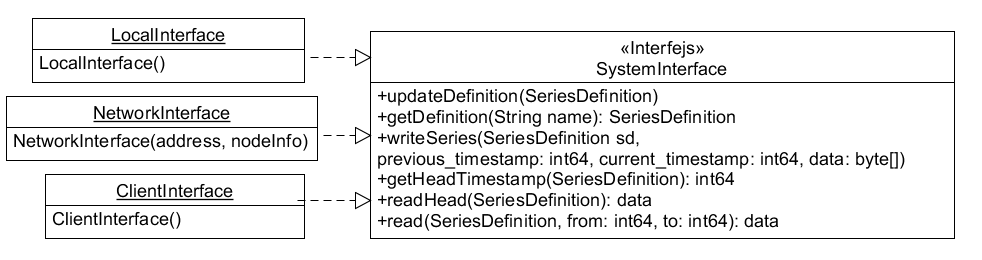
\includegraphics[width=16cm]{uml_ifc}
		\caption{Diagram UML interfejsu wraz z trzema istniejącymi klasami implementującymi go.}
		\label{fig:uml_ifc}
	\end{figure}

\textit{LocalInterface} jest implementacją która operacje wykonuje przy użyciu tylko i wyłącznie lokalnych zasobów, tj. korzystając z funkcjonalności \textit{SeriesDB}. Jeśli jakiś ciąg nie jest dostępny na węźle, zwróci on taką informację. Jest więc mechanizmem dostępu do operacji udostępnianych przez bazę lokalnie.

\textit{ClientInterface} wykonuje operacje biorąc pod uwagę cały klaster. W przypadku gdy nie jest on odpowiedzialny za dany węzeł, połączy się z innym by zrealizować tą operację. Wszelakie operacje redefinicji są przesyłane do węzłów odpowiedzialnych.

\textit{NetworkInterface} jest zdalną reprezentacją interfejsu jakiegoś węzła. Nie wykonuje on operacji poza połączeniem się z innym węzłem i zlecenia wykonania mu jakiejś operacji.

Kolejnym, bardzo istotnym elementem modułu \textit{ifc} jest klasa \textit{NetworkCallInbound}. Przetwarza ona komunikację sieciową na gniazdku na wywołania interfejsu. To, którego interfejsu uwzględnionego na rysunku \ref{fig:uml_ifc} dotyczy zapytanie, zależy od charakteru połączenia sieciowego z \textit{ifc}. Istnieją dwie kategorie połączeń --- międzywęzłowych oraz klienckich. Po drugiej stronie połączenia klienckiego znajduje się moduł którego zadaniem jest zapisanie bądź odczytanie danych, bez wnikania w strukturę klastra. Zostanie on obsłużony więc przy pomocy implementacji \textit{ClientInterface}, który zadba o to aby jego żądanie zostało zrealizowane, choćby niektóre węzły nie działały. Do tego celu \textit{ClientInterface} będzie musiał połączyć się z innymi węzłami. W przypadku tego połączenia międzywęzłowego \textit{NetworkCallInbound} korzystać będzie z implementacji \textit{LocalInterface}. Dzieje się tak gdyż węzeł realizujący polecenia klienckie wie z którym węzłem należy się połączyć (dzięki bazie \textit{gossip}). Dodatkowo, wymagana jest logiczna topologia pełnej siatki, tak aby każdy węzeł mógł łączyć się z dowolnym innym.

Podejście takie wprowadza więc dodatkową zaletę systemu --- każdy z węzłów w klastrze może realizować polecenia dla klientów, i nie jest istotne to który węzeł tą operację wykona. Pozwala to na tolerancję awarii ze strony klientów. Gdy jeden węzeł zawiedzie, klienci mogą połączyć się z innym i dalej korzystać z bazy. Możliwe jest również zawężenie puli węzłów ,,interfejsów`` chociażby przy pomocy mechanizmów sieciowych takich jak firewall czy router. 

Dzięki zastosowaniu podejścia interfejsu możliwe było zastosowanie jednego kodu (tak jak i protokołu) obsługującego połączenia między węzłami jak i połączenia klienckie. Klasa \textit{NetworkCallInbound} w momencie tworzenia jej pobiera jako parametr interfejs za pomocą którego realizować będzie zdekodowane polecenia.

Aby jednak w sposób sprawny obsługiwać polecenia \textit{ClientInterface} musi dysponować pewną logiką i zasadami realizacji poleceń klienckich. Tak więc w przypadku odczytu danych klasa ta sprawdza czy aby to węzeł aktualnie wykonujący polecenie nie dysponuje tymi danymi. W takim wypadku nie będzie potrzeby otwierania \textit{NetworkInterface}, a polecenie może będzie mogło zostać wykonane przy użyciu \textit{LocalInterface}. Kod, ze względu na wykorzystanie interfejsów języka Java, pozostaje identyczny. \textit{Gossip} dysponuje funkcją zwracającą listę węzłów odpowiedzialnych za dany ciąg z precedencją dla węzła lokalnego - tak więc jeśli będzie to węzeł lokalny, zostanie on zwrócony jako pierwszy. Klasa \textit{InterfaceFactory} zwraca interfejs po wskaźniku na węzeł, albo \textit{NetworkInterface} jeśli to węzeł zdalny, albo \textit{LocalInterface} jeśli jest to węzeł który wykonuje to polecenie. Dodatkowo \textit{InterfaceFactory} implementuje pamięć podręczną połączeń, aby nie wykonywać nawet i kilku połączeń TCP na jedno żądanie, gdyż bardzo ucierpiałaby na tym wydajność bazy.

Nieco inne obostrzenia występują w przypadku pobrania wartości maksymalnego stempla czasowego. W tym przypadku odpytywane są wszystkie odpowiedzialne węzły, możliwe bowiem, że któryś z nich zwrócił awarię, a informacja którą w tym przypadku zwrócimy klientowi może doprowadzić do awarii, ponieważ bardziej aktualne węzły zignorują te zapisy. W takiej sytuacji węzeł który uległby awarii dysponowałby różnymi danymi niż pozostałe, czyli system uległby desynchronizacji. Podobnie wygląda sytuacja zapisów, czy aktualizacji definicji ciągu. Kod realizujący w tym wypadku zapis przedstawiono na listingu \ref{lst:ifc_writeseries}.

\begin{listing}
\linespread{1} \small \lstinputlisting[label=lst:ifc_writeseries, language=Java, captionpos=b, caption=Operacja dopisania rekordu w \textit{ClientInterface}.]{ifc_writeseries.java} \linespread{\WorkLineSpread} \normalsize
\end{listing}

W dowolnej chwili, jeśli łączność z innym węzłem w ramach \textit{NetworkInterface} zawiedzie, informacja ta zostanie przekaza do modułu \textit{gossip} celem śledzenia awarii węzłów.

	\subsection{Protokoły sieciowe}
Celem skomunikowania się klienta z bazą danych oraz elementów klastra ze sobą wzajemnie, niezbędne jest zdefiniowanie protokołu sieciowego. Szczególnie istotne jest precyzyjne określenie protokołu za pomocą którego klienci będą łączyć się z bazą, wysyłać swoje polecenia i otrzymywać odpowiedzi.

Ponieważ wszystkie te rodzaje komunikacji dokonują się na jednym porcie TCP, wymagany jest jakiś sposób na odróżnienie ich po sobie. Klient sieciowy jako pierwszy bajt wysyła właśnie typ połączenia,  za pomocą którego \textit{netdispatch} przekieruje połączenie do odpowiedniego modułu. Jeśli będzie to bajt:
	\begin{itemize}
		\item 0 --- jest to przychodzący komunikat \textit{gossip},
		\item 1 --- jest to połączenie danych międzywęzłowe. Należy uruchomić \textit{NetworkCallInbound} z implementacją \textit{LocalInterface},
		\item 2 --- jest to połączenie od klienta bazy. Należy uruchomić \textit{NetworkCallInbound} z implementacją \textit{ClientInterface}.
	\end{itemize}

Najprostszym wariantem jest połączenie typu \textit{gossip}. Polega ono na wysłaniu czterobajtowego znacznika długości komunikatu, a następnie samego komunikatu. Komunikat taki jest zserializowaną za pomocą mechanizmów języka Java klasą zawierającą opis danych i dokładnego charakteru komunikatu, co jest do przetworzenia bezpośrednio przez moduł \textit{gossip}.

W przypadku bajtu 1 lub 2 sytuacja jest znacznie bardziej skomplikowana. Co prawda protokół, ze względu na zastosowany interfejs, w obu wypadkach pozostaje taki sam, jednak niemożliwe staje się zastosowanie mechanizmów serializacji języka Java do przesyłania komunikatów, gdyż wtedy z bazy korzystać mogliby tylko klienci napisani w tym języku programowania.

Innymi słowy, protokół ten definiowany jest bardziej przy pomocy przenośnej funkcjonalności języka Java, jaką jest \textit{DataStream}, pozwalający zapisać zmienne w postaci bajtów, interpretowalnych przez mechanizmy również innych języków programowania.

Po pierwszym bajcie, za pomocą którego \textit{netdispatch} ustala charakter połączenia, \textit{NetworkCallInbound} oczekiwać będzie na kolejny bajt, opisujący rodzaj komendy. Czas oczekiwania ustalony jest na 4 sekundy, tak więc maksymalnie tak długo połączenie może być utrzymywane bez realizacji żadnej komendy. Jeśli klient nie zamierza wykonać żadnego polecenia, zaleca się aby od razu zamknął połączenie. 

W dalszej części tego rozdziału zamieszczono specyfikację protokołu. Pisana jest ona przy użyciu charakterystycznych typów danych, sprecyzowanych w tabeli \ref{tab:datatypes}. Dodatkowy typ (definicja ciągu), pojawiający się w specyfikacji poleceń, opisano w tabeli \ref{tab:intp}.

\begin{table} \centering \begin{tabular}{|c|c|p{8cm}|}
\hline Nazwa & Rozmiar w bajtach & Opis \\ \hline
byte & 1 & bajt bez znaku \\
short & 2 & liczba ze znakiem w reprezentacji uzupełnień do dwóch\\
int & 4 & liczba ze znakiem w reprezentacji uzupełnień do dwóch\\
long & 8 & liczba ze znakiem w reprezentacji uzupełnień do dwóch\\
string & więcej niż 2 & najpierw short z długością ciągu, dalej ciąg bajtów w kodzie zmodyfikowanym UTF-8. \\
\hline \end{tabular}
\caption{Opis typów danych używanych w specyfikacji (typ zapisu \textit{big endian})} \label{tab:datatypes} \end{table}

\begin{table} \centering \begin{tabular}{|c|c|p{8cm}|}
\hline Nazwa & Typ & Opis \\ \hline
replicaCount & int & Ilość replik ciągu \\
recordsize & int & Rozmiar pola danych rekordu \\
generation & long & generacja definicji \\
autoTrim & long & wartość opcji \textit{autoTrim}, opisanej w rozdziale \ref{sec:anatomy} \\
tombstonedOn & long & wartość znacznika skasowania ciągu , opisanego w rozdziale \ref{sec:anatomy} \\
options & string & opcje dla sterownika \textit{LFD} zarządzającego ciągiem \\
seriesName & string & nazwa ciągu \\
\hline \end{tabular}
\caption{Opis definicji ciągu w reprezentacji sieciowej (pola podane w kolejności)} \label{tab:intp} \end{table}

Gdy \textit{NetworkCallInbound} zostanie uruchomiony dla danego połączenia, odbiera bajt i parametry komendy.

Jeśli to bajt 0, to jest to polecenie pobrania definicji ciągu. Parametrem jest \textit{string} zawierający nazwę ciągu. Następnie serwer zwróci bajt statusu. Jeśli będzie to 2, to oznacza że definicja nie występuje w systemie. Jeśli jest to 1, to wystąpił wewnętrzny błąd węzła lub klastra (należy ponowić zapytanie), a jeśli 0 to serwer odeśle do klienta definicję\footnote{format opisano w tabeli \ref{tab:intp}}.

Jeśli jest to bajt 1, to jest to polecenie zdefiniowania (bądź redefinicji ciągu). Po tym klient wysyła definicję, która ma zostać wprowadzona do systemu. Jeśli redefinicja przebiegnie pomyślnie, klient odeśle bajt 0, jeśli wystąpi błąd --- bajt 1.

Jeśli to bajt 2, to jest to polecenie pobrania maksymalnego stempla czasowego. Jeśli zostanie zwrócony bajt 1 to wystąpił wewnętrzny błąd. Zwrócony bajt 2 to kod nieodnalezienia definicji ciągu. Zwrócony bajt 3 to informacja o tym że definicja którą przesłał klient, jest przestarzała (zmiana generacji). Jeśli zwrócony jest bajt 0, to następny wysłany zostanie przez serwer long z znalezionym stemplem czasu.

Jeśli to bajt 3 to jest to polecenie dopisania rekordu. Następnie klient wysyła definicję szeregu oraz znacznik czasowy poprzedniego zapisu i stempla czasowego bieżącego rekordu w formacie long (łącznie dwa znaczniki). Następnie wysyła długość pola danych w formacie short oraz pole danych rekordu. Do bazy zostanie zapisany rekord złożony z stempla czasowego bieżącego rekordu i danych.
Teraz serwer odpowiada jednym bajtem statusu. Jeśli będzie to 4, to długość pola danych jest niezgodna ze specyfikacją ciągu. Jeśli jest to 3, to definicja którą przesłał klient, jest przestarzała. Jeśli ciąg nie został znaleziony, zwrócone zostanie 2, jeśli wystąpił ogólny błąd --- 1. Jeśli operacja zostanie zrealizowana poprawnie, zwrócony zostanie bajt 0.

Jeśli jest to bajt 4, to jest to polecenie odczytania zakresu. Następnie klient wysyła definicję szeregu oraz dwa znaczniki zakresu odczytu, czyli znacznik ,,od`` i ,,do`` (łącznie dwa znaczniki) w formacie long. Następnie serwer odpowiada bajtem statusu, gdzie 1 to ogólny błąd, 2 to nieodnaleziony ciąg, 3 to przestarzała definicja, zaś 4 to błąd zakresu (chociażby ,,do`` mniejsze od ,,od``). Zero to kod transmisji pomyślnej --- wysłana zostanie następnie seria danych w postaci stempla czasowego typu long i bajtów danych --- tyle ile wynosi rozmiar pola danych w tym ciągu. Transmisję tą kończy wartość -1 typu long.

Jeśli jest to bajt 5, to jest to polecenie odczytania najnowszego rekordu. Następnie klient wysyła definicję szeregu. Następnie serwer odpowiada bajtem statusu, gdzie 1 to ogólny błąd, 2 to nieodnaleziony ciąg, 3 to przestarzała definicja. Zero to kod transmisji pomyślnej, wysłany zostanie następnie rekord w postaci stempla czasowego typu long i bajtów danych --- tyle ile wynosi rozmiar pola danych w tym ciągu. Transmisję tą kończy wartość -1 typu long. Jeśli w danym ciągu nie ma ani jednego rekordu, -1 zostanie odesłane natychmiastowo.

Komunikacja międzywęzłowa przebiega na identycznych zasadach, z zastrzeżeniem takim że na te komendy węzeł odpowiada bez konsultacji z innymi węzłami, jednak to zagadnienie z punktu widzenia czysto klienckiego jest mniej interesujące.

	\docsection{Instalacja i konfiguracja systemu}  \label{sec:system_service}
	W tym rozdziale ujęto zasady służące do konfiguracji klastra tak, aby pracował on w sposób stabilny i szybki. Przede wszystkim wyjaśniono wymagania sprzętowo-programowanie, to w jaki sposób należy konfigurować pojedyncze węzły. Ujęto również zagadnienia dotyczące naprawy węzłów w przypadku awarii. Kolejno opisano zasady projektowania schematu bazy, czyli konkretnych ciągów. Wspomniano również o zasadach dostępu klienckiego.

		\subsection{Wymagania sprzętowo-programowe}
Ze względu na możliwość pracy w systemach heterogenicznych baza nie wymaga konkretnego systemu operacyjnego. Minimalnym wymaganiem programowym jest to, aby system dysponował implementacją standardu Java w wersji przynajmniej 1.7. Wymagany jest również dostęp do sieci (przynajmniej jeden interfejs sieciowy), oraz miejsce dyskowe. Należy tak zaplanować dostępne miejsce na dysku, aby w całości był się w stanie zmieścić na nim największy ciąg, który ma być przechowywany w systemie, gdyż baza nie dzieli ciągów między węzły.

Konsekwentnie, należy określić katalog w systemie plików, w którym baza będzie składować dane. Przede wszystkim należy określić, na jakiej partycji znajdować się będą dane. Nie powinna być to partycja z nadmiarowym RAID, jeśli planuje się korzystać z wielu węzłów i funkcji replikacji danych.

Od strony sieci wymaga się, aby każdy z węzłów mógł nawiązać połączenie z dowolnym innym. Najprostszym sposobem realizacji jest umieszczenie wszystkich węzłów w jednej sieci lokalnej, nadając im różne adresy IP. Sieć musi zapewniać możliwość prowadzenia komunikacji typu TCP. Klient systemu bazodanowego musi móc połączyć się przynajmniej z jednym, dowolnym klientem. Zalecane jest, aby mógł połączyć się z kilkoma (na wypadek awarii jednego z węzłów dostępowych).

Sieć, w której jest instalowana baza, ze względu na uwarunkowania bezpieczeństwa i brak wsparcia dla uwierzytelniania i szyfrowania, musi znajdować się w jednym, zaufanej podsieci IP. W przypadku systemów, które nie mogą spełnić tego warunku ze względów lokalowych, należy zastosować technologię VPN w celu stworzenia wirtualnej sieci. Obecne na rynku rozwiązania VPN pozwalają zestawić połączenie szyfrowane, więc w zapewniony jest warunek zarówno zaufania jak i pojedynczej sieci IP.

Należy zwiększyć na systemach uniksowych liczbę maksymalnych otwartych deskryptorów plików na proces, do wartości równej przynajmniej 120\% maksymalnej liczby ciągów trzymanych w pamięci cache, ponieważ na jeden otwarty ciąg przypada jeden otwarty deskryptor, zaś zapytania odczytu generują dodatkowe deskryptory.

Spełnienie warunków istotne jest zwłaszcza przy wdrożeniach lokalnych, gdzie baza występować będzie blisko systemów pomiarowych, a warunki nie zawsze są pod kontrolą administratora czy instalatora. Ze względu na pełną kontrolę środowiska, dostępną na infrastrukturze serwerowej SMOK, na której baza będzie wdrożona, warunki te są spełnione.

	\subsection{Planowanie klastra}
Przede wszystkim rozplanowując układ klastra należy najpierw określić iloma węzłami dysponuje się, oraz jaka jest ich ,,moc przerobowa``. Pojemność dyskowa powinna być proporcjonalna do pamięci operacyjnej oraz mocy procesora, ze względu na to, że obciążenie tych komponentów będzie wprost proporcjonalne do pojemności.

Mając określone węzły, należy przypisać im konfigurację sieciową, tj. adres IP i port na którym mają one działać. Dany zestaw powinien być dostępny z sieci lokalnej. Port można pozostawić domyślny (tj. 8886), gdyż będzie go można zawsze dostosować w pliku konfiguracyjnym.

Kolejnym, najważniejszym w zasadzie, etapem projektowania klastra jest przypisanie węzłom przedziałów odpowiedzialności. Ponieważ węzeł dla ciągu ustala się po wyniku funkcji mieszającej, należy przyporządkować im zakresy zbioru wartości tej funkcji. Oznacza to ,,pokrojenie`` między węzły zakresu liczb odpowiadającego typowi \textit{long} języka Java\footnote{czyli liczby całkowitej od -9223372036854775808 do 
9223372036854775807 włącznie}. Należy zachować zasadę, że ,,kawałek`` przestrzeni powinien być  proporcjonalny do przestrzeni dyskowej. ,,Kawałek`` oznacza się poprzez podanie wartości, od której rozpoczyna się przedział danego węzła, tak więc wartość -9223372036854775808 musi wystąpić w jednym z węzłów. Do wyznaczenia takiego schematu może posłużyć arkusz kalkulacyjny. Pewną propozycję dla przykładowych danych przedstawiono w tabeli \ref{tab:sample_clusterplan}.

\begin{table} \centering \begin{tabular}{|c|c|c|}
\hline IP & Miejsce na dane & Początek przedziału \\ \hline
192.168.0.2 & 100 GB & -9223372036854775808 \\
192.168.0.3 & 150 GB & -8627931621305730000 \\
192.168.0.4 & 500 GB & -7734770997982150000 \\
192.168.0.5 & 300 GB & -4757568920236910000 \\
192.168.0.6 & 2 TB & 7437050790207630000 \\
\hline \end{tabular}
\caption{Przykład projektu małego klastra} \label{tab:sample_clusterplan} \end{table}

Kolejnym krokiem jest wyznaczenie węzłów startowych, do których inne  węzły będą się łączyć celem pobrania informacji o stanie sieci. Węzły takie stanowią ,,punkty zborne`` przy inicjalizacji klastra. Zamiast wybrać jeden z nich, można też wybrać dwa albo trzy, należy jedynie upewnić się, że one same będą łączyć się z innym węzłem startowym. Taka ścieżka ,,węzłów startowych dla węzłów startowych`` powinna zawierać cykl, ze względu na możliwe awarie węzłów podczas startu. Przykład takiego rozplanowania przedstawiono na rysunku \ref{fig:start_nodes}.

	\begin{figure}[h]
		\centering 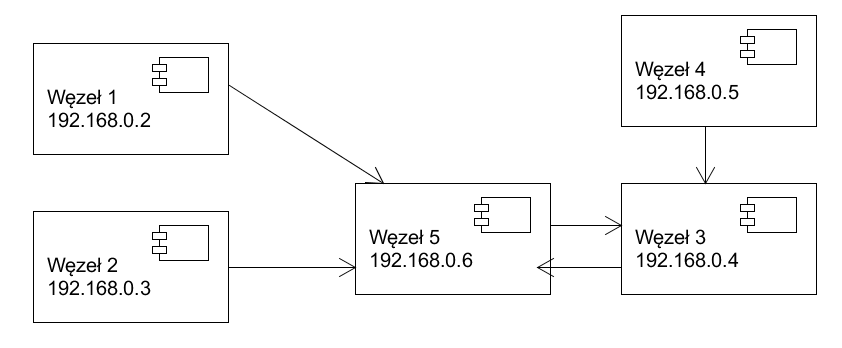
\includegraphics[width=16cm]{start_nodes}
		\caption{Przykład układu węzłów startowych. Strzałka oznacza węzeł, który dany węzeł ma za startowy (np. węzeł 1 łączy się do węzła 5).}
		\label{fig:start_nodes}
	\end{figure}

Na tym etapie projektowanie węzła jest zakończone i można przystąpić do instalacji oraz konfiguracji oprogramowania bazodanowego.

	\subsection{Instalacja i konfiguracja węzła}
\label{sec:part:sample_clusterplan}
Program wykonywalny bazy danych dostępny jest w postaci pliku \textit{jar} zawierającego zastosowane zewnętrzne biblioteki\footnote{Apache Commons IO oraz Google GSON, dzięki czemu nie jest wymagana ich osobna instalacja.}. Wymagane jest skopiowanie tego pliku, wraz z referencyjnym plikiem konfiguracyjnym \textit{config.json} do jednego katalogu. Katalog ten będzie katalogiem uruchomieniowym dla procesu bazy danych.

\begin{table}  \begin{tabular}{|c|p{9cm}|}
\hline Nazwa & Opis \\ \hline
bootstrap\_node\_ip & Adres IP lub nazwa hosta węzła startowego. \\
bootstrap\_node\_port & Port, na którym nasłuchuje węzeł startowy. \\
node\_ip & Adres IP interfejsu sieciowego, na którym ma nasłuchiwać ten węzeł. \\
node\_port & Port TCP, na którym ma nasłuchiwać ten węzeł. \\
nodehash & Początek przedziału tego węzła. \\
seriesdata\_path & Ścieżka do katalogu, w którym przechowywane będą ciągi główne. \\
seriesmeta\_path & Ścieżka do katalogu, gdzie przechowywane będą metadane. \\
seriesdata\_repair\_path & Ścieżka do katalogu, gdzie przechowywane będą ciągi pomocnicze, służące do naprawy. \\
gc\_grace\_period & Czas (w sekundach) bezpieczny służący do usuwania ciągów.  Interpretację szerzej opisano w p. \ref{sec:part:gcollector}. Rozsądnie jest pozostawić domyślną wartość wynoszącą 1 tydzień. Wartość tego parametru powinna być identyczna na wszystkich węzłach danego klastra.\\
series\_in\_memory & Maksymalny rozmiar cache dla ciągów. Tyle metadanych ciągów maksymalnie będzie przechowywanych w pamięci operacyjnej. \\
\hline \end{tabular}
\caption{Pola konfiguracyjne pliku \textit{config.json}} \label{tab:config_fields} \end{table}

Po skopiowaniu plików do katalogu uruchomieniowego należy otworzyć w edytorze tekstowym plik \textit{config.json}. Zawiera on szereg pól, które objaśniono w tabeli \ref{tab:config_fields}.

Rozbicie danych na trzy grupy: dane zasadnicze, metadane i ciągi pomocnicze, pozwala dostosować system plików pod konkretny typ danych, rozpatrując to jak często będzie do nich realizowany dostęp. Do zasadniczych danych zwykle będzie to zapis, a starsze pliki będą odczytywane stosunkowo rzadko. Dobrym rozwiązaniem może być dla tego typu danych system plików z kompresją. Z kolei metadane są małymi plikami, które muszą być załadowane względnie szybko, więc można im przydzielić szybki system plików oparty na urządzeniach SSD. W przypadku instalacji na systemie Windows należy pamiętać o stosowaniu znaków escape (np. $C:{\backslash}{\backslash}sciezka$ zamiast $C:{\backslash}sciezka$). Należy upewnić się, że katalogi podane w konfiguracji rzeczywiście istnieją, a baza będzie miała prawo do ich zapisu.

Pole \textit{series\_in\_memory} należy dostosować do rozmiaru pamięci RAM w systemie, a przede wszystkim do liczby maksymalnych otwartych deskryptorów plików. Nie stanowi to dużego problemu w systemach Windows (brak twardych limitów deskryptorów \cite{Russinovich:Limits}), jednak może stanowić kłopot w systemach uniksowych, w których takie limity są określone\cite{limits.conf}, acz mogą być modyfikowane. Wartość docelową należy ustalić biorąc 120\% wartości \textit{series\_in\_memory}.

Żeby uruchomić węzeł, należy przejść do katalogu uruchomieniowego i wykorzystać do uruchomienia maszynę Javy. Przykład uruchomienia węzła będącego startowym przedstawiono na rysunku \ref{fig:start_zero1}.

	\begin{figure}[h]
		\centering 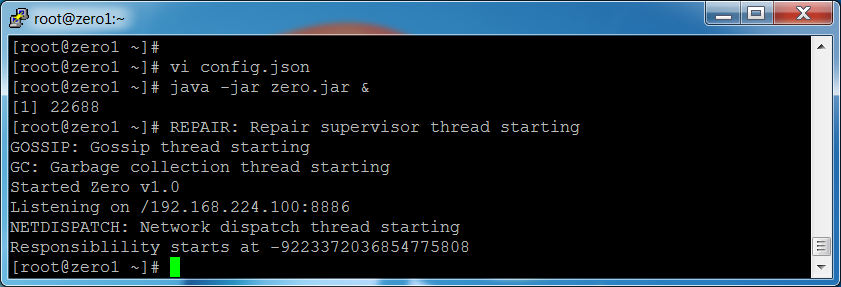
\includegraphics[width=14cm]{start_zero1}
		\caption{Uruchomienie węzła startowego ,,zero1``}
		\label{fig:start_zero1}
	\end{figure}

Celem wyjaśnienia sposobu projektowania i instalacji systemu przedstawiono tutaj konfigurację systemu, który posłużył później do celów testowych. Składać będzie się on z trzech węzłów o identycznych parametrach sprzętowych --- jednordzeniowy procesor Intel\footnote{Maszyny zostały zrealizowane jako maszyny wirtualne pracujące w środowisku QEMU/KVM. Podczas testów przydzielono maszynom maksymalny priorytet na poziomie hipernadzorcy celem minimalizacji zakłóceń.} o taktowaniu 2.3 GHz, dysk twardy 15 GB oraz 1 GB pamięci RAM. Systemem operacyjnym będzie GNU/Linux CentOS 7. Na dane przeznaczymy ok. 10 GB, biorąc pod uwagę konieczność pozostawienia miejsca dla systemu operacyjnego.

Pierwszym etapem projektowania jest stworzenie tabeli na wzór \ref{tab:sample_clusterplan}. Biorąc pod uwagę to że wszystkie węzły są równorzędne, przestrzeń wartości (równą $2^{64}$) można rozdzielić między nie równo. Wyniki tego etapu zamieszczono w tabeli \ref{tab:example_clusterplan}.

\begin{table} \centering \begin{tabular}{|c|c|c|}
\hline IP & Miejsce na dane & Wartość przedziału \\ \hline
192.168.224.100 & 10 GB & -9223372036854775808 \\
192.168.224.101 & 10 GB & -3074457345618258604 \\
192.168.224.102 & 10 GB & 3074457345618258601 \\
\hline \end{tabular}
\caption{Projekt klastra testowego (przykładowego)} \label{tab:example_clusterplan} \end{table}

Kolejnym krokiem jest ustalenie grafu węzłów startowych. Ze względu na prostotę tej instalacji można określić jeden węzeł startowy --- niech będzie nim 192.168.224.100. Pozostałe węzły będą się łączyć do niego celem początkowej ,,koordynacji``.

Po instalacji docelowego oprogramowania na maszynach przeprowadzono ich konfigurację. Była ona na wszystkich węzłach podobna, wystąpiły jedynie różnice w adresacji IP interfejsów oraz początków przedziałów. Drugą istotną różnicą było uzupełnienie ustawień węzła startowego w 192.168.224.101 i 192.168.224.102. Konfigurację przedstawiono na rysunku \ref{fig:example_config}. Konfigurację 192.168.224.102 utworzono analogicznie.

Teraz należy przeprowadzić uruchomienie węzłów. Jako pierwszy powinien zostać uruchomiony węzeł 192.168.224.100. Jest to wymagane, gdyż węzły które będą uruchamiane później muszą być się w stanie z nim połączyć\footnote{celem uproszczenia wywodu wcześniej poprawnie skonfigurowano firewall. Opis tej operacji wykracza poza temat ninejszej pracy.}. Tak więc węzły uruchomiono w kolejności 100, 101, 102. Wraz z każdym uruchomieniem możemy obserwować jak wszystkie węzły aktualizują swoją bazę danych, wykrywając nowe węzły. Większą pauzę (kilka sekund) zaobserwować można między startem 102 a wykryciem go przez 101, co związane jest z tym że propagacja przez węzeł 100 może zająć do 4 sekund. Stan konsoli po uruchomieniu węzła 101 w momencie gdy informacje są już rozesłane przedstawia rysunek \ref{fig:after_101_start}.

	\begin{figure}[h]
		\centering 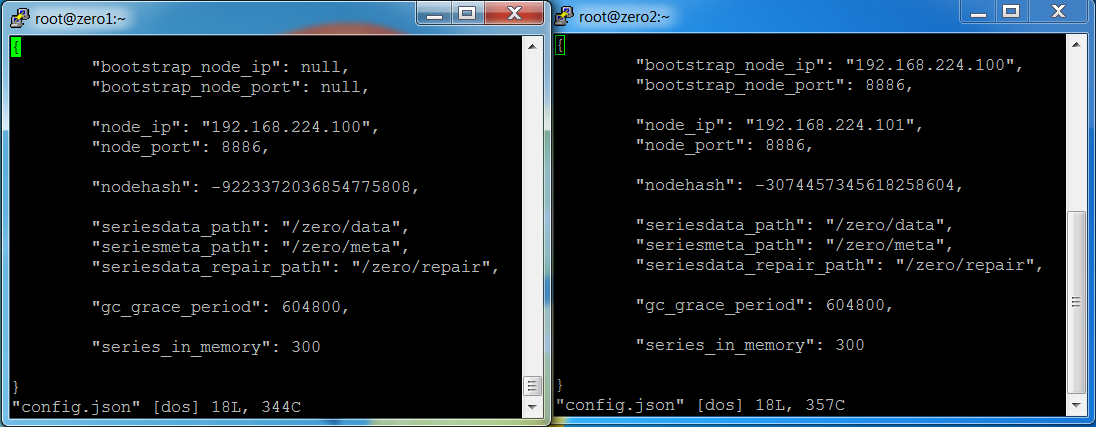
\includegraphics[width=15cm]{example_config}
		\caption[Przykład konfiguracji dwóch węzłów]{Konfiguracja dwóch węzłów. Po lewej stronie konfiguracja 192.168.224.100, po prawej 192.168.224.101.}
		\label{fig:example_config}
	\end{figure}

	\begin{figure}[h]
		\centering 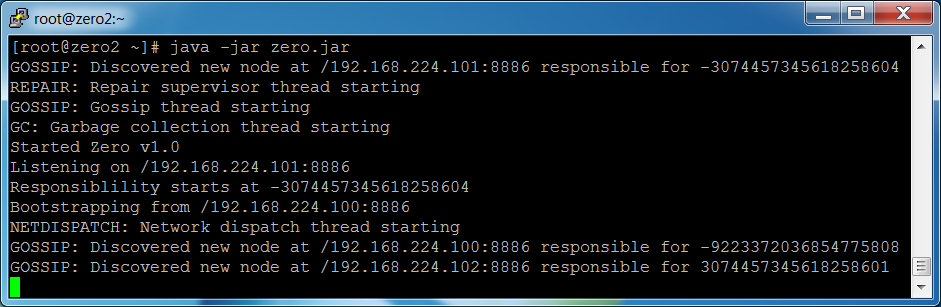
\includegraphics[width=15cm]{after_101_start}
		\caption[Zrzut ekranu konsoli węzła]{Konsola węzła 192.168.224.101 po uruchomieniu węzła 192.168.224.102. Węzeł najpierw ,,odkrywa`` siebie samego (101), później odkrywa węzeł startowy (100) gdy łączy się do niego, a na samym końcu otrzymuje informację o węźle 102, który dołączył do klastra jako ostatni.}
		\label{fig:after_101_start}
	\end{figure}

W tym momencie --- czyli gdy każdy węzeł wie o każdym --- klaster gotów jest do pracy w roli bazy danych systemu kontrolno-pomiarowego, a węzły oczekują na komendy.

Zatrzymania programu dokonuje się poprzez wymuszone ,,zabicie`` procesu. Program jest zaimplementowany jako \textit{crash-only software}\cite{Candea:2003}, to jest oprogramowanie którego jedynym sposobem zatrzymania jest nagłe i wymuszone przerwanie pracy. Przerwanie pracy programowi w dowolnej chwili, czy to przez awarię czy przez zatrzymanie z woli użytkownika, nie grozi nieodwracalnym uszkodzeniem danych.

Skonfigurowany tutaj przykładowy klaster posłuży później do testów.

	\subsection{Naprawa klastra i węzła} \label{sec:cluster_repair}
W pracy klastra może wydarzyć się sytuacja, że jeden z węzłów ulegnie awarii i przestanie reagować na komendy. Może być to związane z awarią sprzętową lub programową na systemie działającym jako węzeł.

Niezależnie od przyczyny awarii, obsługa bazy w przypadku awarii jest bardzo prosta. Sama usterka może być dłuższy czas niezauważona, ze względu na wbudowaną tolerancję na awarie węzłów klastra. Z tego powodu zalecane jest korzystanie z zewnętrznych narzędzi monitorujących pracę poszczególnych węzłów. Są one standardowymi elementami wdrożenia systemów klastrowych.

Pamiętać należy o tym, że jedynym elementem identyfikującym węzeł w systemie jest początek jego przedziału odpowiedzialności. Inne węzły potraktują nawet nowy komputer, legitymujący się tą samą wartością przedziału, jako stary element klastra.

Gdy awaria została już usunięta na poziomie sprzętowo-systemowym, tj. jednym elementem który należy przywrócić jest działanie procesu bazy danych, należy rozpatrzyć czas awarii. Inny jest sposób postępowania w przypadku, gdy sumaryczny czas awarii węzła był mniejszy od czasu bezpiecznego (związanego z kasowaniem metadanych). Jeśli czas awarii był mniejszy, to należy po prostu uruchomić proces węzła i pozwolić mu samemu zsynchronizować się z resztą klastra. Należy jedynie upewnić się że w pliku konfiguracyjnym znajduje się taka sama wartość przedziału jak w węźle który uległ awarii.

Jeśli natomiast czas awarii był większy, lub system uległ awarii do tego stopnia że niezbędne było przywrócenie systemu z kopii zapasowej czy nowa instalacja, należy skonfigurować bazę ,,na czysto``, pamiętając jedynie o zgodności wartości przedziału z węzłem który uległ awarii. Jeśli system ocalał, a jedynie czas awarii był większy od czasu bezpiecznego, wystarczy wyczyścić katalogi danych, metadanych i ciągów naprawczych, a następnie uruchomić program.

		\subsection{Projektowanie i zapis ciągów}
		\label{sec:one_client_one_series}
W klasycznych bazach danych SQL projektowanie tzw. schematu bazy danych jest zagadnieniem złożonym. W prezentowanej bazie, ze względu na jej relatywną prostotę, jest to wyzwanie nieco prostsze, jednak w dalszym ciągu nietrywialne. Przedstawiono tutaj kilka zasad i propozycji tyczących się definiowania i planowania ciągów.

Przede wszystkim pierwszym zadaniem powinna być analiza systemu pomiarowego. Jeden ciąg bazy odpowiada najczęściej jednemu punktowi pomiarowemu, zbieranemu przez jeden czujnik. Błędem byłoby stworzenie jednego ciągu dla dwóch czy trzech czujników, zwłaszcza gdy ich działanie nie jest za sobą zsynchronizowane. Dopuszczalna jest natomiast sytuacja czy jeden ciąg reprezentuje dwa pomiary, które ze względu na konstrukcję systemu muszą być wykonywane jednocześnie i obsługiwane przez jeden komponent.
	
W ogólności, w systemie musi być określona odpowiedzialność elementu zapisującego za konkretny ciąg. Nie może występować sytuacja w której dwa elementy próbują zapisać do jednego ciągu. Związane jest to z tym, że element zapisujący musi pamiętać ostatni stempel czasowy zapisu, natomiast przy więcej niż jednym elemencie taka synchronizacja jest niemożliwa lub bardzo trudna. Nie stanowi ono problemu w systemie SMOK, gdyż agent obsługi obiektu odpowiedzialny jest za wszystkie ciągi danej lokalizacji. Jest to jednocześnie jedyny element który będzie zapisywał dane na rzecz tego obiektu i jest uruchomiony ciągle, doskonale spełnia więc te założenia.

Praktycznym przykładem planowania schematu bazy może być prosty system grzejąco-chłodzący składający się z grzejnika, klimatyzatora oraz czujnika temperatury wewnętrznej. Wartości z czujnika temperatury dopisywane byłyby do jednego z ciągów. Odnośnie stanów binarnych grzejnika i klimatyzatora (włączony lub wyłączony) możliwe są dwa rozwiązania. W pierwszym z nich stany każdego z urządzeń tworzyłyby osobne ciągi, w drugim oba stany zapisane na kolejnych bitach liczby dopisywane byłyby do wspólnego ciągu.

Baza danych posługuje się dedykowanym protokołem dostępu, niezbędne jest więc zastosowanie elementu ,,zbieracza`` danych. Jego zadaniem byłoby przetwarzanie protokołu czujników i systemu automatyki na protokół bazy. Pełniłby on także rolę ,,bufora`` danych, zapewniając że żadne dane nie zostaną utracone podczas zapisu, oraz pełniłby rolę abstrakcji dla nietypowego sposobu zapisu wykorzystywanego przez bazę (konieczność pamiętania definicji ciągu i ostatniego stempla czasowego zapisu). Rolę takiego elementu w systemie SMOK pełni agent obsługi obiektu. Działając cały czas jest w stanie buforować zapisy. 

Innym zagadnieniem może być ,,symulacja`` rekordów o różnych długościach. Ponieważ ciąg pozwala jedynie na rekordy o stałej długości, można go zasymulować definiując dwa ciągi. Załóżmy że mamy system rejestrujący wartości zespolone lub wielowymiarowe (np. przesuw frezarki, odczyty zespołu akcelerometrów), przy czym znakomita większość pomiarów to wartości rzeczywiste. Zamiast definiować pojedynczy ciąg zawierający wartości zespolone o dwukrotnie większym rozmiarze, można zdefiniować dwa ciągi: jeden od części rzeczywistych, drugi od urojonych. Ponieważ większość pomiarów będzie rzeczywista, to będą one trafiać jedynie do ciągu rzeczywistego. Jeśli pojawi się jakaś część urojona, może być ona dopisana do ciągu liczb urojonych, z identycznym stemplem czasowym co odpowiadająca jej część rzeczywista. Ideę takiego rozwiązania przedstawiono na rysunku \ref{fig:variable_length_record}.

	\begin{figure}[h]
		\centering 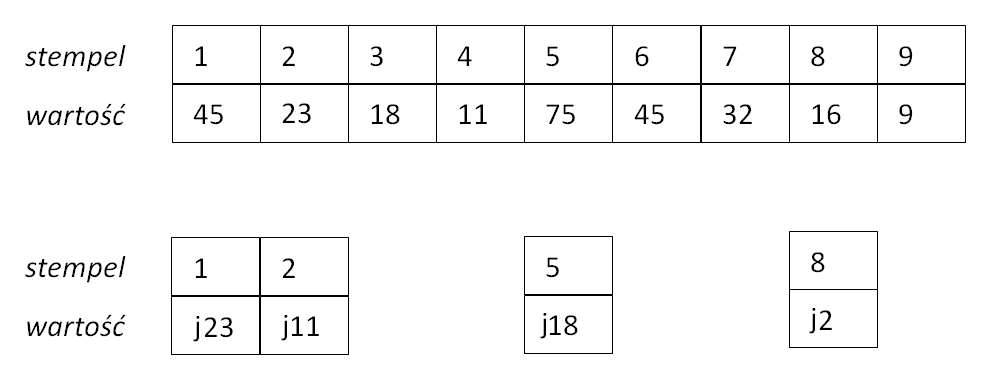
\includegraphics[width=14cm]{variable_length_record}
		\caption[Przykład implementacji ,,rekordu o zmiennej długości``]{Przykład implementacji ,,rekordu o zmiennej długości``. Pomiar dla stempla czasowego 1 można przedstawić jako $45+j23$, zaś dla stempla 3 jako $18$.}
		\label{fig:variable_length_record}
	\end{figure}

Określenie precyzyjnych schematów i wytycznych nie jest możliwe do określenia ścisłymi schematami i wytycznymi, podobnie jak dla baz relacyjnych i wymaga w dużej mierze doświadczenia i intuicji.

	\subsection{Interfejs Python}
Celem demonstracji możliwości skorzystania z funkcji przygotowywanej bazy przy użyciu języków programowania innych niż Java, stworzono także interfejs napisany w języku Python. Sprawdza się on jako język służący do zespalania różnych elementów systemu. Charakteryzuje się ponadto szybkością tworzenia oprogramowania. Również, idąc  z duchem języka, stworzony interfejs charakteryzuje się prostotą. Na listingu \ref{lst:python_ifc} przedstawiono program dopisujący wartość do ciągu. Oczywiście nie jest konieczne wypisywanie wszystkich węzłów, ponieważ wystarczy jedynie kilka aby interfejs skorzystał z innego, jeśli wystąpią problemy z połączeniem.

Interfejs dysponuje również opcją wyrównywania obciążeń --- łączy się najpierw do losowego hosta z podanej listy, ze względu na ekonomię skali powinno wyrównywać obciążenie węzłów.

\begin{listing}
\linespread{1} \small \lstinputlisting[label=lst:python_ifc, language=Python, captionpos=b, caption=Skrypt dopisujący rekord do ciągu]{test_write.py} \linespread{\WorkLineSpread} \normalsize
\end{listing}

Znaczące części systemu SMOK stworzone zostały właśnie w języku Python. Tyczy się to zwłaszcza komponentów które odpowiedzialne są za zapis pomiarów w obecnej bazie danych. Dzięki temu integracja tworzonego rozwiązania z resztą systemu jest prostsza niż w przypadku skorzystania z interfejsu dostępnego w innym języku programowania. Wymagałoby to dodatkowych nakładów pracy. Przeprowadzono integrację bazy danych z testową wersją systemu SMOK, umieszczając w niej wcześniej zebrane dane. Na rysunkach \ref{fig:smokscreenshot2} i \ref{fig:smokscreenshot3} przedstawiono zrzuty ekranu z pracy testowej bazy w systemie SMOK.

	\begin{figure}[H]
		\centering 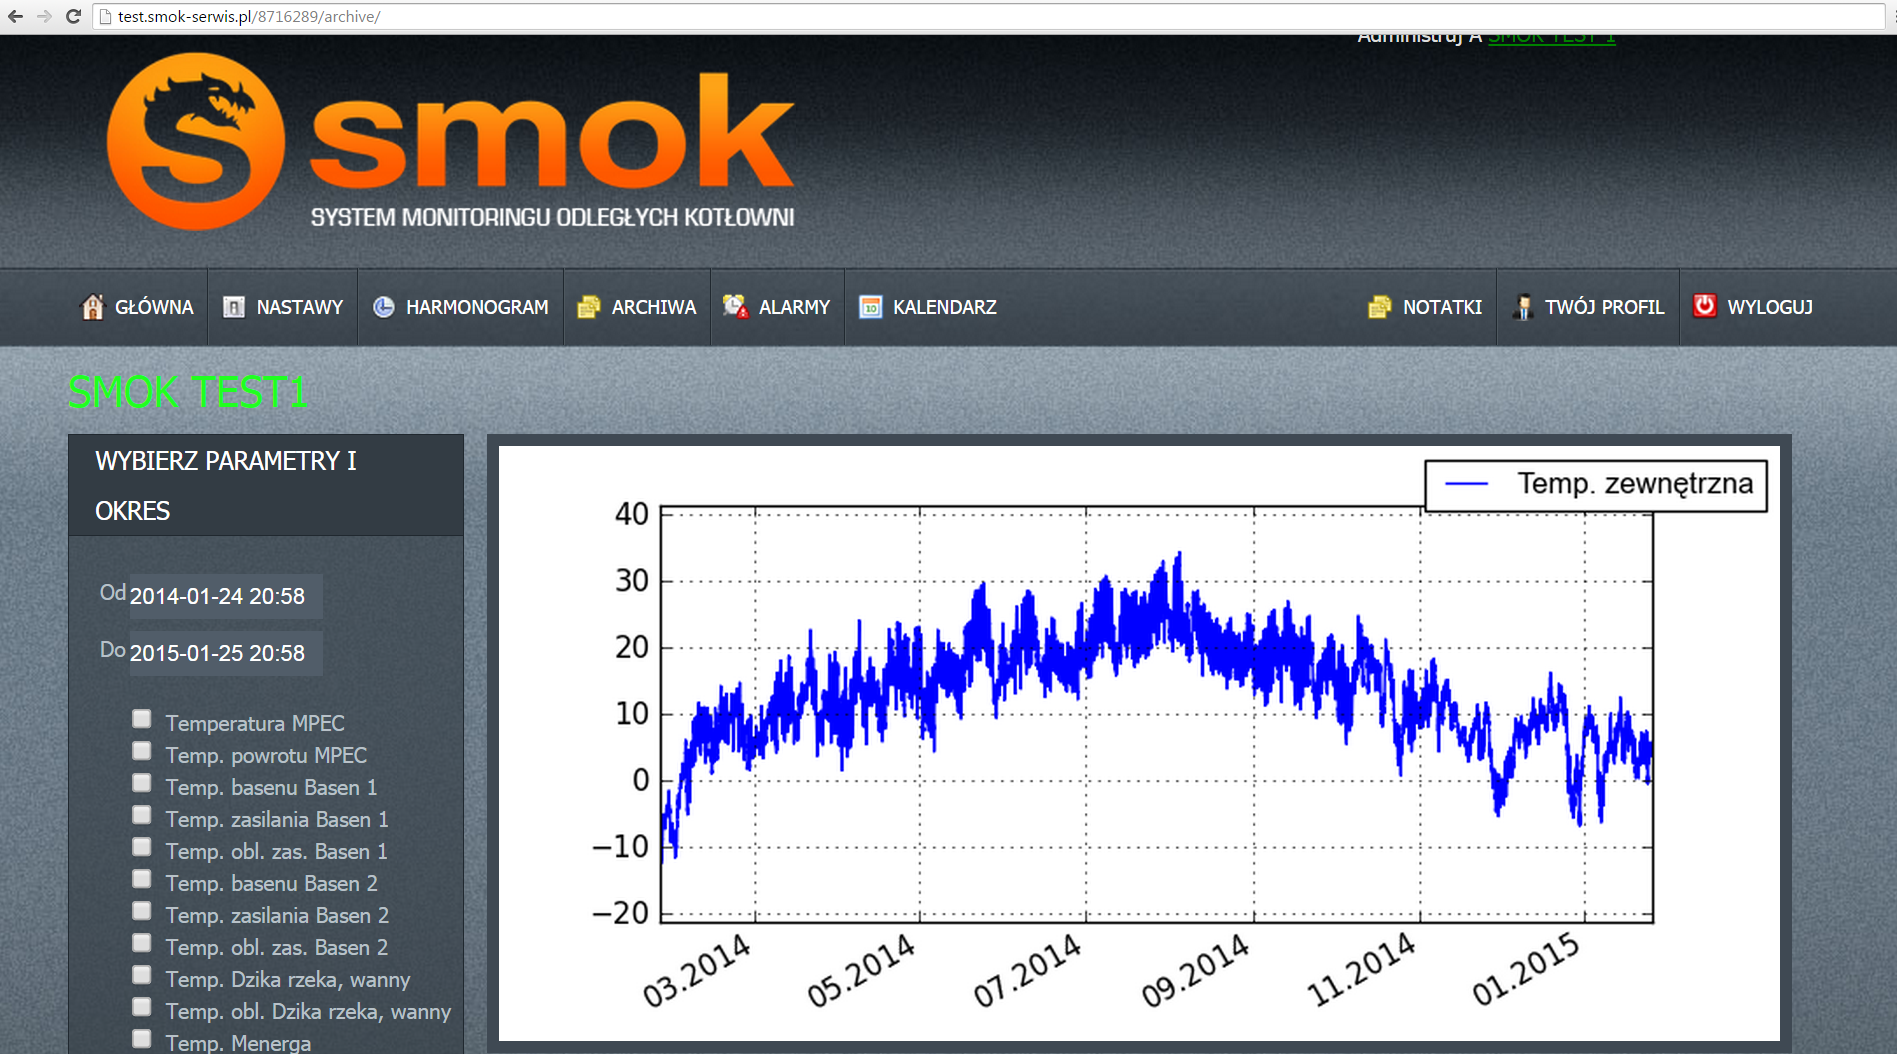
\includegraphics[width=15cm]{smokscreenshot2}
		\caption[Zrzut ekranu z pracy bazy na testowej platformie SMOK]{Zrzut ekranu z pracy bazy na testowej platformie SMOK. Sporządzono wykres temperatury zewnętrznej od końca stycznia 2014 do 2015.}
		\label{fig:smokscreenshot2}
	\end{figure}

	\begin{figure}[H]
		\centering 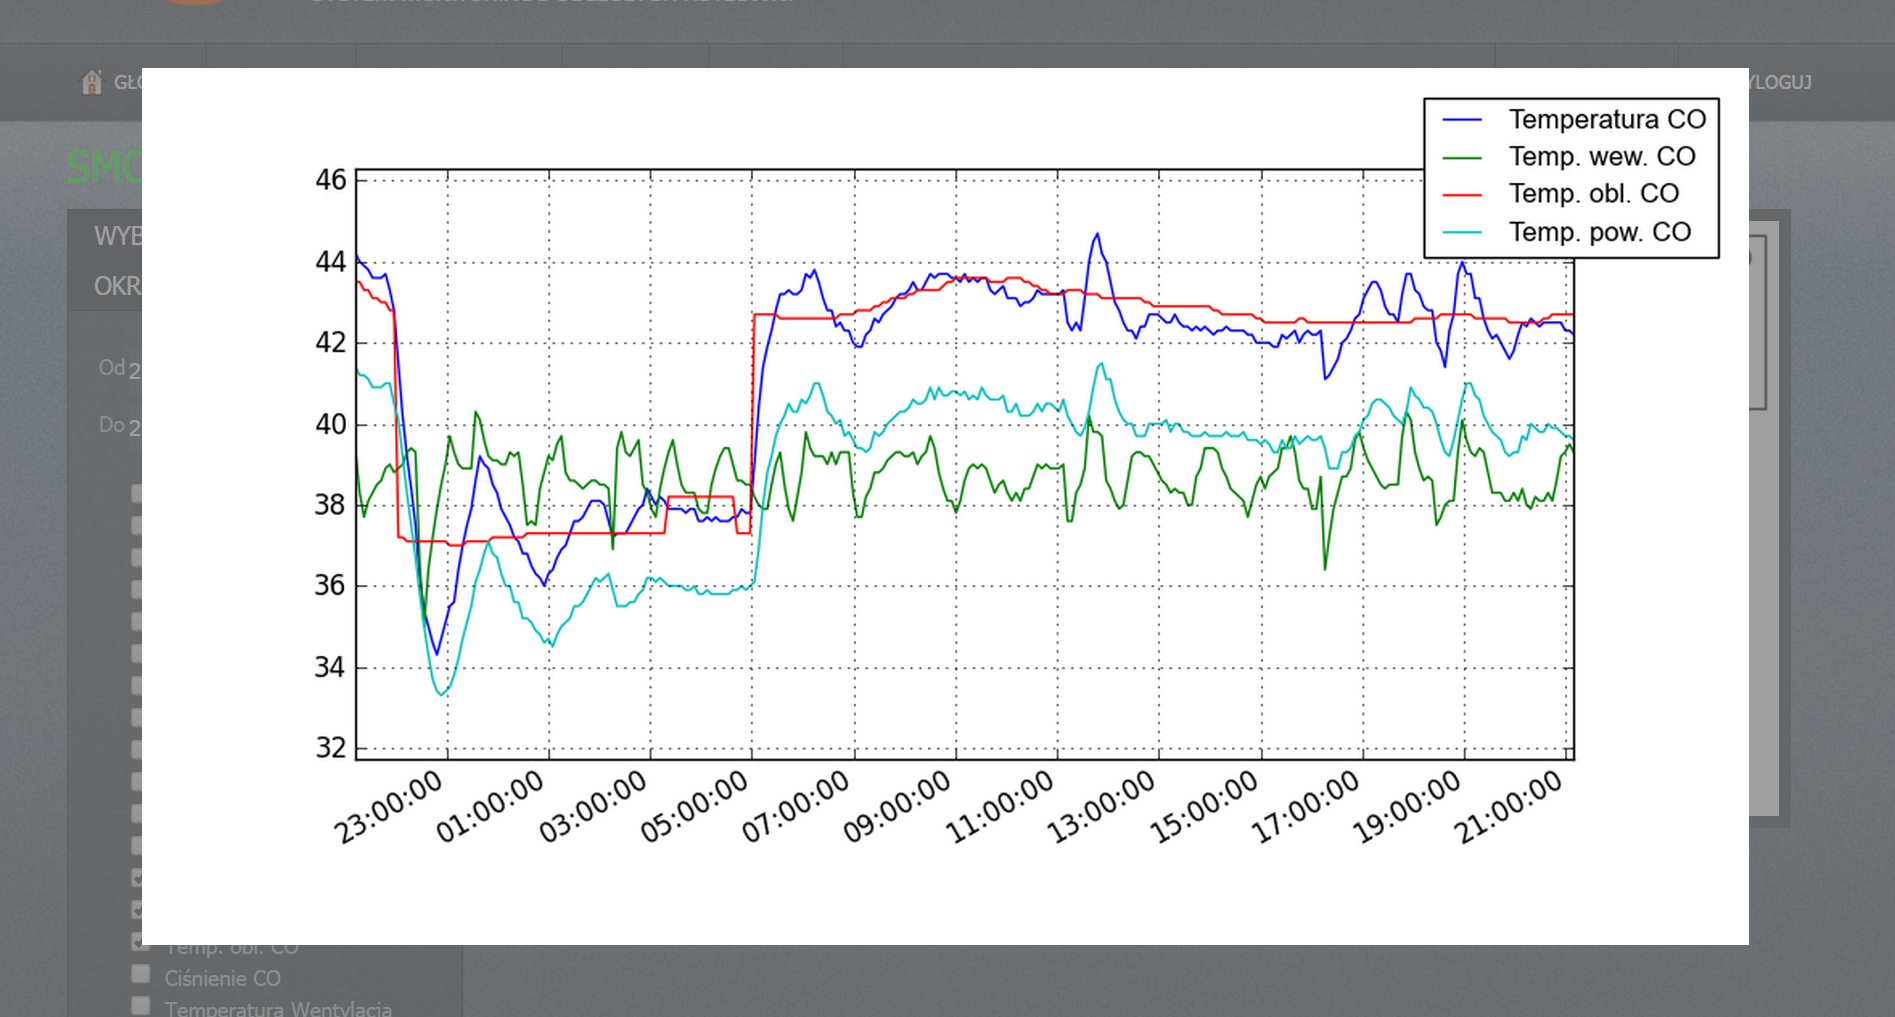
\includegraphics[width=15cm]{smokscreenshot3}
		\caption[Zrzut ekranu z pracy bazy na testowej platformie SMOK]{Zrzut ekranu z pracy bazy na testowej platformie SMOK. Sporządzono wykres temperatur obiegu centralnego ogrzewania.}
		\label{fig:smokscreenshot3}
	\end{figure}

	\docsection{Testy systemu}

Zdecydowano się na przeprowadzenie trzech testów, które miały sprawdzić różne aspekty pracy stworzonego systemu bazodanowego. Pierwszym z nich był test określający w jaki sposób system reaguje na wzrost obciążenia. Wyniki testu pozwolił ustalić komponent systemu, który ma największy wpływ na szybkość rozwiązania.
Drugi test pozwalał na określenie zachowania systemu w trakcie awarii, oraz jego możliwości samonaprawy. Trzeci test miał na celu stwierdzenie czy rozwiązanie nadaje się wydajnościowo do zastosowania w systemie kontrolno-pomiarowym SMOK.

Środowisko testowe jest identyczne z tym, którego konfigurację przedstawiono w rozdziale \ref{sec:part:sample_clusterplan}. Należy zauważyć, że skonfigurowane elementy są maszynami wirtualnymi, tak więc w celu minimalizacji zakłóceń pomiarowych związanych z obciążeniem fizycznej maszyny ustalono im priorytet wyższy niż pozostałym maszynom wirtualnym na tym serwerze.

Dodatkowo, skonfigurowano wirtualną maszynę kliencką o adresie 192.168.224.103. Będzie ona kierować zapytania do klastra przy użyciu interfejsu Python.

	\subsection{Zależność czasu obliczeń od liczby ciągów}
Pierwszym testem, który przeprowadzono, był test skalowalności mający na celu zbadanie właściwości zbudowanej bazy pod względem skalowalności. Testem tym był równoległy zapis do wielu ciągów. 
	Pomiar dla pojedynczej ilości ciągów polegał na stworzeniu pewnej liczby (parametryzowanej) wątków systemu operacyjnego. Zadaniem każdego z wątków było zapisanie 1000 rekordów do własnego ciągu, to jest każdemu wątkowi przyporządkowany był jego własny ciąg i własne połączenie TCP. Następnie, gdy wątki zostały utworzone, zostały w jednej chwili uruchamiane, od tego momentu liczony był sumaryczny czas zapisu. W momencie gdy ostatni wątek zapisujący kończył, czas był kończony.

Każdy ciąg miał 2 repliki i rozmiar pola danych 4 bajty. Pomiaru dla każdej ilości ciągów dokonywano 3 razy, wybierając medianę. Badano tutaj zależność czasu wykonania całej operacji od ilości równoczesnych zapisów. Oczekuje się, że wąskim gardłem systemu będą operacje I/O, tak więc fakt że węzły mają po jednym procesorze nie będzie problemem.

Zapis realizowano poprzez klienta wielowątkowego napisanego w języku Python.
	\begin{figure}[h]
		\centering 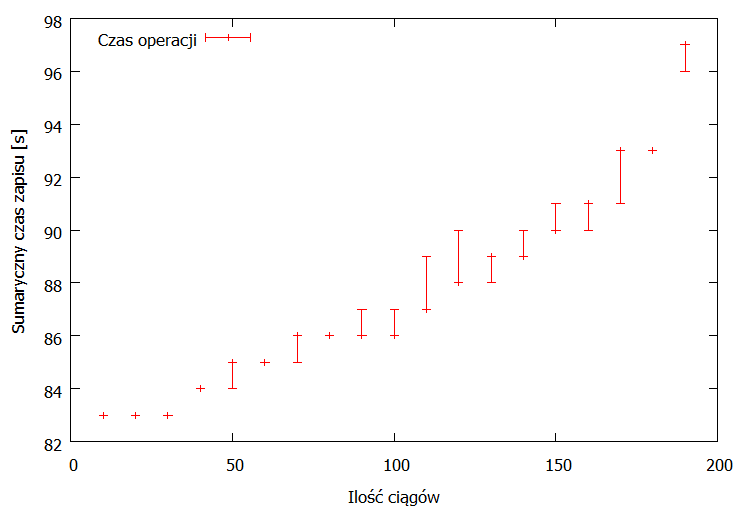
\includegraphics[width=14cm]{test_plot1}
		\caption[Wyniki pomiaru zależności ilości równoległych zapisywanych ciągów od czasu trwania całej operacji]{Wyniki pomiaru zależności ilości równoległych zapisywanych ciągów od czasu (w sekundach) trwania całej operacji. Słupki błędów oznaczają minimum i maksimum.}
		\label{fig:test:plot1}
	\end{figure}

Wyniki eksperymentu przedstawiono w postaci wykresu na rysunku \ref{fig:test:plot1}. Widoczna jest  korelacja dodatnia ilości ciągów i czasu całej operacji. Sumarycznie jest ona jednak bardzo niewielka, bo stanowi przyrost o 16\%\footnote{$\frac{97,10 s - 83,10 s}{83,10 s}$} przy 19-krotnym zwiększeniu obciążenia. Test został zaprojektowany w celu ustalenia charakteru zrównoleglenia stworzonej bazy danych. Cele te zostały osiągnięte, wyniki bowiem należy zinterpretować następująco:
\begin{enumerate}
	\item Rozwiązanie jest bardzo dobrze zrównoleglone pod względem obliczeniowym
	\item Prędkość rozwiązania zależy w głównej mierze od przepustowości sieciowej
\end{enumerate}
	Punkt 1 oznacza, że baza danych nie generuje znaczącego obciążenia w obszarze obliczeń i dostępu do dysku. Przyrost czasu na obliczenia był bowiem niewielki mimo znaczącego wzrostu obciążenia. Oznacza to, że stopień optymalizacji kodu jest zadowalający. Punkt 2 wymaga szerszego omówienia. Węzły posiadały procesory jednordzeniowe, czyli system miał łącznie 3 procesory, a mimo tego nie zaobserwowano znaczącego przyrostu czasu. Większość czasu wątki spędzały w uśpieniu, oczekując albo na operację I/O dysku, albo na operację sieci. Spodziewano się przynajmniej liniowego przyrostu czasu. Równoległość w tym teście polegała na zrównoleglaniu przez system operacyjny operacji dyskowych i sieciowych (system nie musi wykonywać ich w zleconej kolejności, ale w kolejności optymalnej). Ilość zapisanych bajtów na dysk była niewielka\footnote{ok. 2,2 MB}, a na jeden ciąg wykonano tylko jedną operację otwarcia pliku ze względu na obecność podsystemu cache. Pozwala to wykluczyć operacje dysku jako źródło wąskiego gardła. Dominującym czynnikiem musiały być tutaj operacje sieciowe, to jest transmisja danych między węzłami, oraz między węzłami a klientem. Wnioskiem testu jest więc to, że przyśpieszenie pracy sieci przyśpiesza działanie klastra szybciej niż ulepszenie procesora czy dysku. Rozmieszczenie klastrów na osobnych fizycznych maszynach z całą pewnością spowolni pracę systemu, jednak nie dysponowano infrastrukturą na której można by określić jak.

	\subsection{Reakcja systemu na awarię}
		Celem sprawdzenia reakcji systemu na awarię przeprowadzono test polegający na zapisie 10 ciągów pomiarowych (C0 -- C9), z zapisem co sekundę. Poziom replikacji każdego ciągu wynosił 2, co oznacza że w systemie obecne będą 2 kopie danych ciągu. W pewnym momencie wyłączono jeden z węzłów systemu (węzeł 3 o adresie 192.168.224.102), aby zasymulować utratę zasilania komputera\footnote{przerwano pracę maszyny wirtualnej za pomocą polecenia \texttt{virsh destroy}.}. Sprawdzono wtedy czas między wysłaniem rozkazu zapisu a jego zrealizowaniem. Wszystkie zapytania testowy klient kierował do węzła .224.100.

	Przeglądając katalogi z danymi ustalono które ciągi znalazły się na którym węźle. Przynależność węzłów do replik ujęto na diagramie Venna przedstawionym na rysunku \ref{fig:venn1}.
	
	\begin{figure}[h]
		\centering 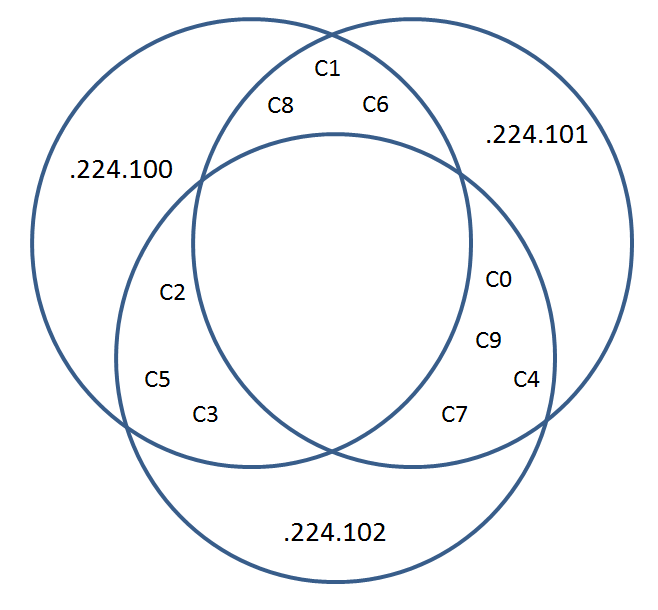
\includegraphics[width=10cm]{venn1}
		\caption{Przynależność ciągów do węzłów}
		\label{fig:venn1}
	\end{figure}

Dla każdego zapisu w każdym ciągu notowano trzy wartości: czas wygenerowania ,,pomiaru``, czas w którym zapis tego pomiaru zaczął być realizowany, oraz czas kiedy zapis został zakończony. Ponieważ awarii uległ węzeł 3 (.224.102), szczególnie interesujące będą wyniki dla węzłów przynależących do tegoż węzła. Ciągi należące tylko do węzłów 1 i 2 będą stanowić grupę kontrolną.

Test przebiegł zgodnie z procedurą:
\begin{enumerate}
	\item $T+0\,s$: Rozpoczęcie testu
	\item $T+68\,s$: Awaria węzła 3
	\item $T+178\,s$: Przywrócenie pracy węzła 3
	\item $T+220\,s$: Koniec zapisów testowych
	\item $T+230\,s$: Wyłączenie programów węzłów
\end{enumerate}

Do zgrubnej analizy wybrano ciągi C0, C1 oraz C2 (każdy z innej grupy). Na podstawie zgromadzonych danych obliczono ile trwał jeden zapis. Poprzez ,,czas trwania zapisu`` rozumiemy tu okres między pobraniem ,,pomiaru``, a zgłoszeniem przez bazę że został w sposób trwały\footnote{Oznacza to, że jeśli po tym momencie wystąpi awaria, to dane przetrwają w bazie danych.} zapisany. Wyniki przedstawiono na rysunku \ref{fig:failtest1}.

	\begin{figure}[h]
		\centering 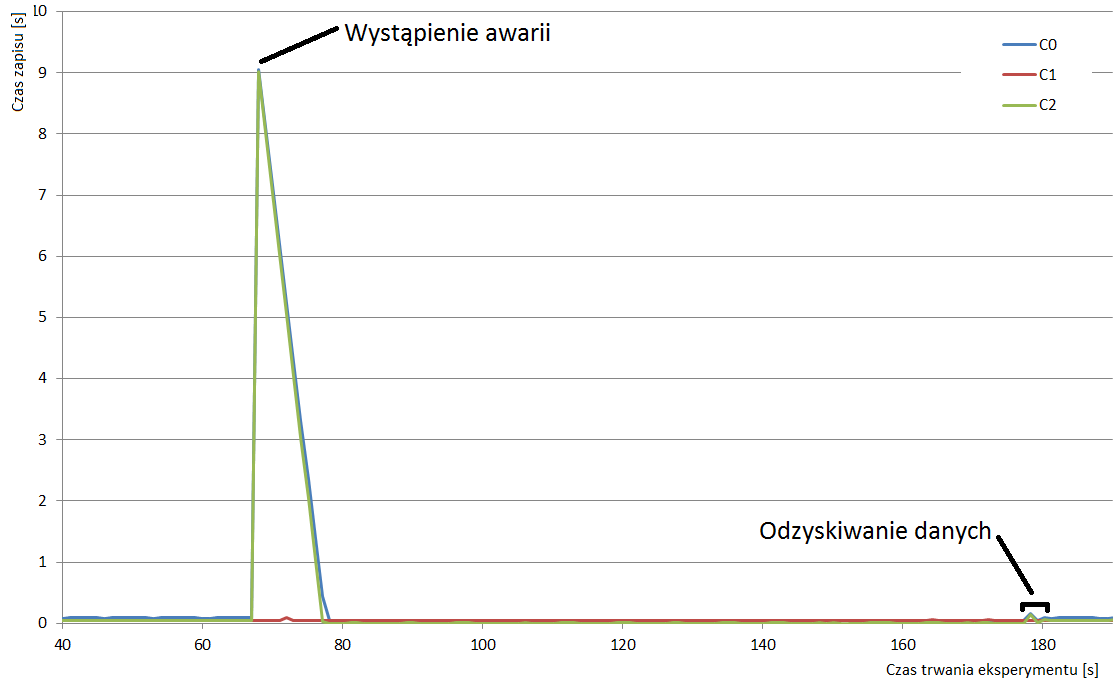
\includegraphics[width=15cm]{failtest1}
		\caption{Czas trwania zapisu w funkcji czasu eksperymentu wyrażonego w sekundach}
		\label{fig:failtest1}
	\end{figure}

Stwierdzić można że przy awarii węzła 3 (68 sekunda) zaobserwowano dla pierwszego zapisu po awarii opóźnienie rzędu 10 sekund. Był to czas, w którym pozostałe węzły stwierdziły, że trzeci uległ awarii i zaktualizowały swoje tabele, aby uniknąć wysyłania temu węzłowi rozkazów zapisu. Czas wykonania zapisu stopniowo zmniejszał się --- wszak przez 10 sekund zgromadzono aż 10 zapisów, które musiały być nadgonione. Potem, aż do przywrócenia działania, czas zapisu nie różni się znacząco od stanu sprzed awarii. W momencie przywrócenia węzła (178 sekunda) obserwuje się krótki pik, związany z obciążeniem systemu próbującego przywrócić brakujące dane. W tym przypadku pobranie brakujących danych przez węzeł 3 z węzłów 1 i 2 zajęło dokładnie 5 sekund\footnote{Nie jest to widoczne na wykresie zaprezentowanym na rysunku \ref{fig:failtest1}. Raport ten uzyskano na podstawie raportu bazy podczas przeprowadzania eksperymentu.}. W obu przypadkach awaria węzła 3 nie miała większego wpływu na opóźnienia w zapisie ciągu C1, który to był obsługiwany przez sprawne węzły 1 i 2. Opóźnienie C1 nigdy nie zwiększyło się powyżej 1, co oznacza że zapisy nie musiały być kolejkowane. Powolny opad piku tłumaczy to że czas liczony był od pobrania pomiaru, więc naturalne pojedyncze opóźnienie opóźni kilka następnych zapisów. Tylko pierwszy zapis po awarii jednak przetwarzany był ok. 10 sekund. Był to czas wymagany na stwierdzenie awarii węzła.

Dziesięciosekundowa przerwa z punktu widzenia systemu SMOK nie jest żadną przeszkodą. Agent obsługi obiektu jest w stanie buforować dane do zapisu przez ten czas, co nie wpłynie negatywnie na jakość świadczonych usług.

Przy końcu eksperymentu porównano dane zgromadzone na węzłach. Wszystkie repliki zgadzały się, co oznacza że system zadziałał w sposób poprawny, a baza jest w stanie naprawić awarię. 


	\subsection{Test obciążeniowy}
Najważniejszym testem, sprawdzającym zdolność bazy do pracy w systemie, był test obciążeniowy. W p. \ref{sec:data_quantity_analysis} ustalono maksymalną liczbę urządzeń i punktów pomiarowych obsługiwanych przez bazę. Niestety, nie dysponowano sprzętem, podobnym do tego na którym w przyszłości mógłby być uruchamiany system bazodanowy. Zdecydowano się więc na symulację wariantu systemu SMOK dla roku 2020 z prognozą dodawania urządzeń co 2 dni. Byłyby to więc 1432 urządzenia, każde po 14 punktów pomiarowych. Dodatkowo, maszyny wirtualne stanowiące składniki klastra wyposażono w drugi procesor wirtualny\footnote{Upewniono się że sumaryczna liczba procesorów nie przekraczała liczby wątków procesora na systemie hipernadzorcy.}. Upewniono się ponadto, że wirtualne urządzenia nie są parawirtualizowane, gdyż przekłamywałoby to testy.

Słowem, stworzono testowego klienta uruchamiającego 1432 połączenia do bazy. Każde połączenie oznaczało zapis co minutę 14 pomiarów do bazy. Ten test miał zweryfikować, czy da się wykonać 1432 połączenia w ciągu minuty. W przypadku przekroczenia czasu zgłaszany był błąd. Niemożność wykonania 14 zapisów na połączenie w ciągu minuty oznaczałaby, że rozwiązanie nie jest w stanie wytrzymać obciążenia. Eksperyment trwał 20 minut. Zdecydowano bowiem (jest to pewne uproszczenie) że jeśli baza wytrzyma to obciążenie przez 20 minut, to będzie je w stanie wytrzymać dowolnie długo. Baza musiała więc być w stanie obsłużyć 20048 zapisów na minutę, to jest ok. 334 zapisów na sekundę.

Czas trwania każdej serii minutowej (to jest wykonania 14 zapisów w obrębie danego połączenia) był zapisywany do pliku. Otrzymano więc 1432 plików zawierających 20 pozycji. Raporty te obrobiono do postaci prezentującej maksimum, minimum oraz wartość średnią. Zaprezentowano je w formie wykresu na rysunku \ref{fig:load_plot}.

	\begin{figure}[h]
		\centering 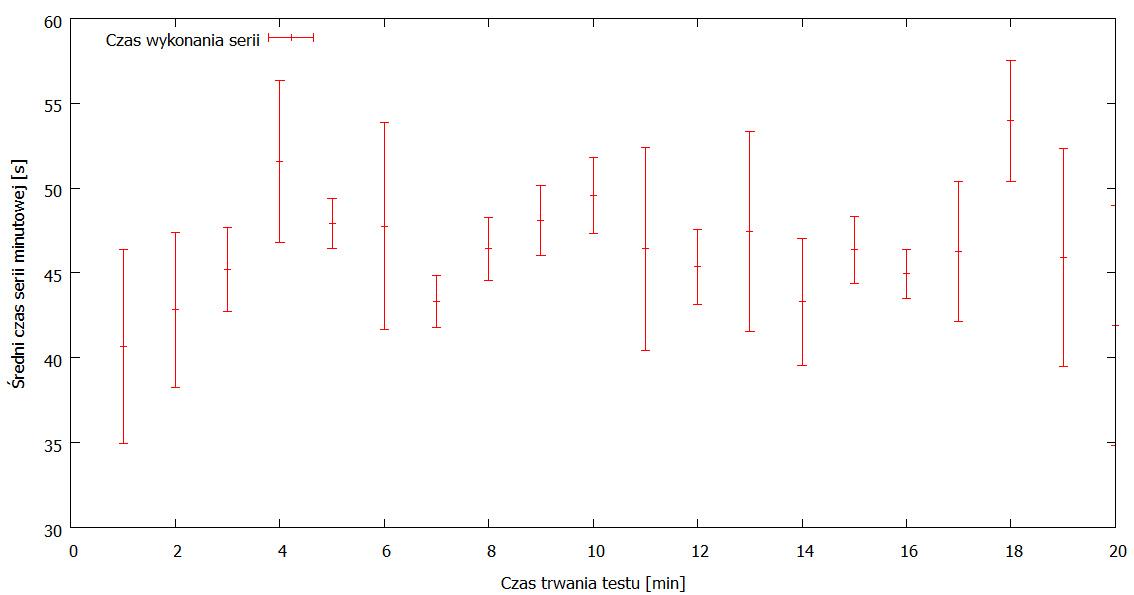
\includegraphics[width=15cm]{load_plot}
		\caption{Wykres obrazujący wyniki testu obciążeniowego}
		\label{fig:load_plot}
	\end{figure}

W jednym tylko przypadku, to jest 18 minuty, czas maksymalny zbliżył się do twardego limitu 60 sekund. W pozostałych przypadkach wartości były poniżej tego progu. Oznacza to, że rozwiązanie to było w stanie podołać założeniom testu. Powziąć można hipotezę, że gdyby dysponowano sprzętem o większej wydajności, możnaby przeprowadzić test z jeszcze większą liczbą urządzeń. Wyniki wskazują również na pewien zapas w czasie, który baza mogłaby spożytkować na ,,nadgonienie`` zapisu danych w przypadku awarii klastra. Baza bowiem sama z siebie wygenerowałaby opóźnienie rzędu ok. 10 sekund, potrzebnych na identyfikację węzła bazy który uległ awarii. 

Pozytywny wynik testu potwierdza możliwość zastosowania rozwiązania w systemie kontrolno-pomiarowym SMOK.

	\docsection{Podsumowanie}

	Problem przechowywania danych w postaci szeregów czasowych jest problemem istotnym. W dobie informacji dokładne opomiarowanie procesu technologicznego, a także przechowywanie i analiza tych danych stanowić może o silnej przewadze nad konkurencją. Wolumen zbieranych danych zwiększa się coraz bardziej, dlatego stabilne i wydajne rozwiązanie bazodanowe stanowi niezbędne uzupełnienie nowoczesnego systemu automatyki przemysłowej.

	Rozwiązania typowo przemysłowe, korzystające ze standaryzowanych interfejsów, coraz częściej wewnętrznie przypominają rozwiązania oparte o systemy Big Data. Działania takie są niezbędne by radzić sobie wydajnie z ilością danych, której tradycyjne systemy nie są w stanie przetworzyć. Z drugiej strony, nietrudno wyobrazić sobie adapter OPC do rozwiązania Big Data, pozwalający z bazy, której przeznaczeniem był nadzór aplikacji internetowej, zbudować system kontrolno-pomiarowy. Jest to możliwe, zwłaszcza że w obu przypadkach bazy przetwarzają szeregi czasowe. W~pewnych warunkach rozwiązania te są tożsame.

Zaprezentowane w pracy rozwiązanie, w kontekście sprzęgnięcia z~systemem SMOK, charakteryzuje szereg zalet w stosunku do istniejących rozwiązań tego typu. Są to:
\begin{itemize}
	\item prosta konfiguracja i instalacja bazy,
	\item redundancja bez konieczności stosowania systemów RAID,
	\item niewielkie wymagania programowe, konieczna jedynie jest maszyna wirtualna języka Java.
	\item dostępność kodu źródłowego i możliwość rozwijania oprogramowania bez ponoszenia kosztów opłat licencyjnych,
	\item łatwa integracja z systemem SMOK (interfejs w języku Python).
\end{itemize}

W pracy przedstawiono rozwiązanie problemu zawierające nowe jakościowo elementy. Zastosowanie algorytmu tabeli mieszającej do kojarzenia węzłów z ciągami spowodowało, że dla użytkownika najtrudniejszą częścią zaprojektowania klastra jest wykonanie kilku prostych działań matematycznych, a konfiguracji --- skopiowanie dwóch plików i dokonanie niewielkich korekt w jednym z nich. Jedynym wymaganiem programowym jest maszyna wirtualna Java, dzięki czemu rozwiązanie działa równie dobrze na systemach Windows co zgodnych z POSIX.

Rozwiązanie to jest autorskie, co umożliwia twórcy pełną kontrolę nad jego rozwojem. Będzie on niezbędny w miarę rozwoju systemu SMOK. Dzięki zastosowaniu bardzo prostej metody zapisu (pliki są ciągami stempli czasowych i wartości pomiarów) można przetwarzać te dane nawet bez konieczności bezpośredniego odpytywania węzła --- wystarczy dostęp do pliku.

Nowatorska metoda sprawdzania spójności ciągu (obowiązek pamiętania definicji szeregu oraz ostatniego stempla czasowego) spowodowała istotne uproszczenie systemu, bardzo szybką detekcję problemów. Pozwala ona przywrócić węzeł, wraz z kompletem danych, po awarii w czasie rzędu kilkunastu minut, nawet w przypadku fizycznego zniszczenia węzła. Pozwala to także na nieprzerwaną pracę w sytuacji, kiedy część danych w klastrze jest fizycznie niedostępna (np. rozległa awaria sieci). Dane te baza przywróci, gdy awaria zostanie usunięta. 

Różnicą w stosunku do rozwiązań opartych o Big Data i klasyfikujących tworzoną bazę jako rozwiązanie dla automatyki jest silna gwarancja przetrwania zapisywanych do niej danych, mimo potencjalnej awarii. Opracowana baza zwraca bowiem potwierdzenie zapisu dopiero, gdy dane zostaną zapisane na nośnik. Dodatkowo, zintegrowana funkcja kasowania starych danych pozwala administratorom na uproszczone przewidywanie ilości miejsca dyskowego, które maksymalnie zużyje klaster. Zapewnia to także możliwość zastosowania rozwiązania do monitorowania aplikacji sieciowych, jak i do przechowywania pomiarów systemu kontrolno-pomiarowego przez zadany okres.

Przeprowadzono również testy. Pierwszy z nich miał na celu określenie charakteru obciążenia, które generuje rozwiązanie. Stwierdzono że największym ograniczeniem dla szybkości działania stworzonej bazy są opóźnienia generowane przez transmisję sieciową między węzłami. Przeprowadzono również test ustalający zachowanie się bazy podczas awarii. Stwierdzono, że zdarzenie takie wygeneruje opóźnienie ok. 10 sekund. Czas ten jest potrzebny na stwierdzenie, że węzeł uległ awarii i nie odpowiada na polecenia. Ostatnim testem był test obciążeniowy, którego wyniki potwierdzają że opracowane rozwiązanie może być z powodzeniem zastosowane w systemie SMOK, nawet w przypadku opóźnienia wygenerowanego przez awarię węzła.

Pewnym mankamentem testów była konieczność przeprowadzenia ich na maszynach wirtualnych, ze względu na niedostępność odpowiedniej klasy sprzętu. Testowe maszyny wirtualne miały dużo mniejszą wydajność od rzeczywistych systemów, na których baza byłaby uruchamiana. Zachowano jednocześnie, na platformie testowej, opóźnienia sieciowe charakterystyczne dla oddalonych systemów. Wpływa to przekłamująco na wyniki, nie można jednak jednoznacznie stwierdzić czy na korzyść czy niekorzyść rozwiązania. 

Rozwiązanie, aby stać się pełnowartościowym rozwiązaniem typu historian wymaga integracji ze standardami przemysłowymi. Niezbędne byłoby stworzenie mostów umożliwiających przekaz danych z sensorów i sterowników przemysłowych do bazy danych. Także bez tego, choć po dostosowaniu infrastruktury akwizycji, stworzona baza może być stosowana w dowolnym systemie kontrolno-pomiarowym --- w ten sposób rozwiązanie będzie zintegrowane z systemem SMOK. Baza oczekuje obecnie na wdrożenie w produkcyjnej wersji zaprezentowanego w pracy systemu kontrolno-pomiarowego. Przede wszystkim dlatego, że przeszła ona pozytywnie wstępne testy, cel pracy można uznać za osiągnięty.

	\textbf{Autor za wkład własny pracy uważa}:
	\begin{itemize}
		\item przegląd literatury związanej z zagadnieniem oraz zapoznanie się z obecnymi rozwiązaniami bazodanowymi,
		\item przeprowadzenie analizy wymagań rozwiązania w kontekście potrzeb systemu SMOK,
		\item zaprojektowanie i wykonanie programu rozproszonej bazy danych oraz modułu klienckiego,
		\item zaprojektowanie protokołu sieciowego niezbędnego do realizacji celów projektu,
		\item zaprojektowanie i przeprowadzenie testów weryfikujących poprawność działania rozwiązania.
	\end{itemize}
	\clearpage

\listoffigures
\listoftables

\clearpage
\bibliographystyle{babplain}
\bibliography{inzynierka}

\section*{Dodatek}
\addcontentsline{toc}{section}{Dodatek}
	Na załączonej płycie CD umieszczono:
	\begin{itemize}
		\item tekst pracy w formacie PDF oraz \LaTeX,
		\item kod źródłowy pracy,
		\item pliki zawierające wyniki pomiarów.
	\end{itemize}

\end{document}